\documentclass[a4paper,11pt,onecolumn,oneside]{regimthese}
\usepackage{algorithm2e}
\usepackage{supertabular}
\usepackage[usenames,dvipsnames]{xcolor}
\usepackage{multirow}
\usepackage{amssymb}
\usepackage{amsbsy}
\usepackage{color}
\usepackage{soul}
\usepackage{amsthm}
\usepackage{natbib}

\usepackage[left=3cm,right=2.5cm,top=3cm,bottom=3cm]{geometry}
\usepackage{incgraph,tikz}
\usepackage{algorithm2e}
\usepackage{supertabular}
\usepackage{multirow}
\usepackage{amssymb}
\usepackage{amsbsy}
\usepackage{amsthm}
\usepackage{caption}
\usepackage{subcaption}
%\usepackage{titlesec}
\usepackage{array}
\usepackage[normalem]{ulem}


% ======================================================= %
\newcounter{commentNum}
\setcounter{commentNum}{0}
%\newtheorem{mydef}{Definition}
% ======================================================= %
% macros
\newcommand{\question}[1]{\addtocounter{commentNum}{1}\vspace{1em}\noindent
\hangindent=0em \textbf{\textcolor{Maroon}{\uline{Comment
\arabic{commentNum}}:~}}{\sffamily{#1}}}
\newcommand{\answer}[0]{\vspace{0.1em} \hangindent=2.3em \textbf{\textcolor{NavyBlue}{\uline{Answer \arabic{commentNum}:~}}}}
\definecolor{darkred}{rgb}{1,.6,.6}
\DeclareRobustCommand\problemline{\bgroup\markoverwith{\textcolor{darkred}{\rule[-0.9ex]{4pt}{3pt}}}\ULon}
\DeclareRobustCommand{\problem}[1]{\problemline{#1}} % soul
%\setcounter{secnumdepth}{-1}
\renewcommand {\theenumi}{\roman{enumi}}
\newcommand{\newlen}[0]{TODO}
%%%%%%%%%%%%%%%%%%%%%%%%%%%%%%%%%%%%%%%%%%%%%%%%%%%%
\definecolor{babyblue}{rgb}{0.54, 0.81, 0.94}
\definecolor{brightgreen}{rgb}{0.4, 1.0, 0.0}
\definecolor{darkorange}{rgb}{1.0, 0.55, 0.0}
\definecolor{pinkpearl}{rgb}{0.91, 0.67, 0.81}
\soulregister\citep7

%#####  Anglais
%\newcommand{\revAnglais}[1]{\sethlcolor{yellow}{\hl{#1}}}
\newcommand{\revAnglais}[1]{#1}
%#####  Faiz
%\newcommand{\revFaiz}[1]{\sethlcolor{green}{\hl{#1}}}
\newcommand{\revFaiz}[1]{#1}
%#####  Karray
\newcommand{\revKarray}[1]{#1}
%\newcommand{\revKarray}[1]{\sethlcolor{babyblue}{\hl{#1}}}



%\renewcommand{\cftpartfont}{\large \bfseries}  
%\renewcommand{\cftchapfont}{\scshape}                          %Bold chapterentries
%\renewcommand{\cftsecfont}{}                           %Typewriter sectionentries
%\renewcommand{\cftsubsecfont}{\itshape}
%\renewcommand{\cftpartpresnum}{\hrule ~\\  \textbf{Part} }


%\ChTitleVar{\Huge\scshape}
 
%\urlstyle{same}
\newtheorem{mydef}{Definition}

\Auteur{Mohamed}{Zarka}{Mastère en informatique}
\President{Prof.}{Chokri \textsc{Ben Amar}}{University of Sfax, Tunisia}{Professeur} 	
\Membres{1}{Prof.}{Slim \textsc{Kanoun}}{University of Sfax, Tunisia}{Professeur}	
\Membres{2}{Prof.}{Fakhreddine \textsc{Karray}}{University of Waterloo, Canada}{Professeur}	
\Membres{3}{Prof.}{Sami \textsc{Faiz}}{University of Manouba, Tunisia}{Professeur}		
\Membres{4}{Prof.}{Adel M. \textsc{Alimi}}{University of Sfax, Tunisia}{Professeur}
\Membres{5}{Dr.}{Anis \textsc{Ben Ammar}}{University of Sfax, Tunisia}{Ph.D.}		

\PhD{Fuzzy Reasoning for Multimedia Semantic Interpretation: 
	\\Fuzzy Ontology Based Model for Video Indexing} 	
	{...............}			
	{Ingénierie des Systèmes Informatiques}
	{informatique}
	{01}
	{Janvier}
	{2014}
%\ThesisDraft 
\newtheorem{definition}{Definition}
\bibpunct{[}{]}{,}{a}{}{;}

\begin{document}
	\dominitoc
	\selectlanguage{english}	
	\PagesCouverture
	%\newpage ~
	\newpage \pagestyle{empty} ~
	\frontmatter{}
	
	\tablefancy
	
	\begin{abstract}

Our thesis work deals with the video indexing based on semantic interpretation (an abstraction of objects or events that figure in a content), more particularly, the semantic indexing enhancement. Various approaches for semantic multimedia content analysis have been proposed addressing the discovery of features ranging from low-level features (color, histograms, sound \revAnglais{frequency}, motions, \dots{}) to high-level ones (semantic objects and concepts). However, these earlier approaches failed to reduce the semantic gap and were not able to deliver an accurate semantic interpretation. Under such a context, exploring further semantics within a multimedia content to improve semantic interpretation capabilities, is a major and a prerequisite challenge.

Towards exploring further semantic information within a multimedia content (other than low-level and semantic concepts one), valuable information (mainly concepts interrelationships and contexts) could be gathered from a multimedia content in order to enhance semantic interpretation capabilities. \revAnglais{Motivated} by a kindred vision of human perception, yet targeting automated analysis of a multimedia content, the multimedia retrieval community addressed more attention to multimedia ontologies.

Aiming to contribute towards this direction, we focus on modeling an automated fuzzy context-based ontology framework for enhancing a video indexing accuracy and efficiency. Key dimensions of this inquiry constitute the main issues addressed by the use of ontologies for multimedia indexing, namely: (1) the knowledge management and evolution, (2) the ability to handle uncertain knowledge and to deal with fuzzy semantics, and (3) the scalability and the ability to process a growing multimedia content volume with a continuous request for a better machine semantic interpretation capacities.

What was accomplished in our study is a novel ontology management which is intended to a machine-driven knowledge database construction. Such a method could enable semantic improvements in large-scale multimedia content analysis and indexing. 

In order to illustrate the semantic enhancement of concept detection introduced by our proposed scalable and generic ontology-based framework, we have conducted different experiments within three multimedia evaluation campaigns: \textsc{TrecVid 2010} (within \emph{Semantic Indexing} Task), \textit{ImageClef 2012} (within \emph{Photo Annotation and Retrieval} Task), and \textit{ImageClef 2015} (within \emph{Scalable Concept Image Annotation } Task).

\par ~
\par ~
\par ~
\par ~
	\textbf{\textit{Keywords:}} Video Indexing, Semantic Interpretation, Fuzzy Ontology, Fuzzy Reasoning, Hierarchical Concept Detector.


\end{abstract}


	\begin{dedicace}
To my parents Salah and Monia,\\
To my wife Bochra and my daughters Mariem and Sarra,\\
To my sisters Rim and Mariem,\\
who have contributed to my work like nobody else.
\\~
\\
%In memory of my aunts Habiba and Cherifa.
\end{dedicace}

	\begin{remerciements}

I was once told that PhD is a long journey of transformation from a \emph{novice} to \emph{professional} researcher. To succeed, an individual can never do it alone; there must be someone who is there for this, providing all the helping hands and supports. I can’t agree more\revAnglais{,} and as for my case, I have a lot of people to thank.

First thanks must be to my supervisor, \emph{Prof. Adel M. Alimi}, who has been truly inspirational throughout my candidature. He always shows me a tireless enthusiasm to meet, discuss, listen and encourage. His invaluable \revAnglais{pieces of advice} and faith make all the difference, and I have been blessed to find in him all the good qualities of a supervisor.  

Many thanks must go to my co-supervisor, Dr. \emph{Anis Ben Ammar}, who has given all the extra guidance and help that prove to be precious in improving the quality of my work. 

I would like to hold this opportunity to express my gratitude and respect to the reviewers \textit{Prof. Sami Faiz} and \textit{Prof. Fakhreddine Karray}, to the exterminator \textit{Prof. Slim Kanoun} and to the chairman \textit{Prof. Chokri Ben Amar}, for their acceptance to evaluate this research work and their valuable remarks and feedback.


A special thanks to Dr. \textit{Nizar Elleuch} and Dr. \textit{Issam Feki} who were always concerned to provide me the necessary conditions for the completion of my thesis.

The \textsc{Regim-Lab} has provided me nice working places with all the much needed facilities, and services, as well as financial supports including travel allowances. Thanks to all the people there who have helped me with many things. 

I would like to acknowledge the financial support of this work by grants 
from General Direction of Scientific Research (DGRST), Tunisia, under the ARUB program.

I thank my wife \emph{Bochra} who is always there for me and makes this whole journey so enjoyable. 

Thanks to all my colleagues \emph{Kais} and \emph{Ghada} who have always given me tremendous supports and encouragement. 

Last, but most importantly, I’d like to dedicate this thesis for my father \emph{Salah} and my mother \emph{Monia} to express my deepest gratitude. They are the best parents who are so willing in giving me the best in life without hoping for anything in return. I am also so blessed to have \revAnglais{such} really loving sisters \emph{Mariem} and \emph{Rim} who gave me so much \revAnglais{support} and encouragement to do well during this candidature.

Above all, I thank my stepfather \emph{Mohamed Hechmi} and my stepmother \emph{Fatma} who have always given me tremendous supports and encouragement. I would like also to thank my stepbrothers  \emph{Kais}, \emph{Hamza}, \emph{Mohamed Hédi}, \emph{Mondher}, \emph{Mohamed Salah} and \emph{Abdelkarim} for supporting me spiritually throughout writing this thesis and \revAnglais{in} my life in general.
\\
\\
\\

Thanks to all\\
Mohamed ZARKA
\end{remerciements}


	\newpage ~

	\lestables		% une commande pour créer la table de matières et la table de figures
	\newacronym{MAP}{MAP}{Mean Average Precision}
\newacronym{GMAP}{GMAP}{Geometric Mean Average Precision}
\newacronym{infAP}{infAP}{Inferred Average Precision}
\newacronym{TrecVid}{TrecVid}{Text REtrieval Conference VIDeo Retrieval Evaluation}
\newacronym{IR}{IR}{Information Retrieval}
\newacronym{CBIR}{CBIR}{Content based image retrieval}


	%\printglossaries

	\mainmatter{}	% commencer la numérotation arabe des pages
	%\introductionfancy
	\regimfancy
			\chapter{General Introduction}
\label{intro}
%\addcontentsline{toc}{chapter}{General Introduction}
%\markboth{General Introduction}{}

	\section{Background and Motivation}
	%\addcontentsline{toc}{section}{Background and Motivation}
	%\sectionmark{Background and Motivation}

	Due to the advance of modern multimedia services and techniques, and the exponential growth of online 
	multimedia data, images and video are overflowing our everyday life. \textsc{Flickr}, as a photo 
	sharing website, stores over 5 billion of images and records an uploading rate of over 3000 
	images per minute\footnote{\texttt{http://blog.flickr.net/en/2010/09/19/5000000000}}. 
	\textsc{YouTube} records a rate of 300 hours  of uploaded videos per 
	minute\footnote{\texttt{https://www.youtube.com/yt/press/fr/statistics.html}}.
	Due to this huge amount of available information, and the diversity of their support and content 
	(newscasts, sports, entertainment programs, movies, documentaries, video surveillance, \dots{}), 
	some problems and difficulties are raising, and a need for efficient tools to access to 
	such amount of multimedia content was strongly stated. 

	The common information retrieval model consists in handling useful information through 
	searching and retrieving from large document collections \citep{Baeza-Yates1999,Manning2008,Grossman2012}. 
	Basically, this model is based on two processes: (1) the indexing process which interprets 
	and stores the content of documents, and (2) the search process which matches a user 
	query and the stored document interpretations in order to evaluate their relevance and 
	output relevant documents.
	
	Image and video indexing is basically based on two different approaches: \emph{Text Based} 
	indexing \citep{Chang1980} and \emph{Content Based} indexing \citep{Smeaton2008}. While the \emph{Text Based}
	means that a content is manually annotated by a text describing contained objects and events, 
	the \emph{Content Based} indexing means the extraction of features (like \revAnglais{color} and shape) in order 
	to automatically detect contained semantic objects.


	Authors in \citep{Hauptmann2007,Wang2008,Hauptmann2007a,Kompatsiaris2008,Darwish2015,Ves2015} 
	pointed out that although the availability of many solutions to fill the so-called \emph{semantic gap} \citep{Hare2006}
	between the automatic interpretation and what human expects from the indexing task; 
	none of them yields satisfactory results:  the problem remains open for further research. 
	In \citep{Smeulders2000}, the \emph{semantic gap} is defined as:

	\begin{mydef}
	\textit{``\dots{} the lack of coincidence between the information that one can extract from the visual 
	data and the interpretation that the same data have for a user in a given situation.''}
	\end{mydef}
	
	As illustrated in figure \ref{introduction_2}, the semantic gap manifests itself as a computational 
	problem for the indexing process.  At the low-level, the raw media refers to an image.%, for our example case. 
	The content-based indexing approaches extract features vectors that represent regions of 
	the image or its whole content. At a higher level, the \emph{objects} are detected through combinations
	of extracted features vectors. \emph{Symbolic labels} may be assigned to these objects (\emph{Crowd} and 
	\emph{Road} for the given example). Nevertheless, such a classical process (based on extracting and 
	combining feature vectors) does not typically capture all the semantics in a given content. In fact, 
	the image context and the relationships between the contained objects contribute to \revAnglais{reach a} high 
	level \revAnglais{of} semantic representation and interpretation of the media content.
	Thus, more than the content analysis is
	requested for a better semantic interpretation: The knowledge structure components showed its capabilities to 
	reach such a higher semantic interpretation. Moreover, the information retrieval \revAnglais{is} more and more supported by
	\revAnglais{knowledge} management processes.

% #, thus, essential in order to give a more understanding of present objects and events, and then, a better interpretation for the content.

	\begin{figure}[ht!]
		\centering
		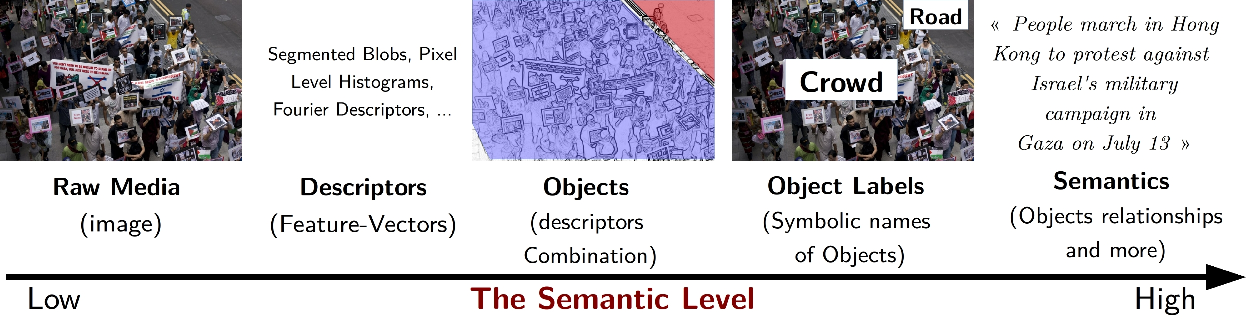
\includegraphics[scale=0.75]{figures/introduction_2.pdf}
		\caption{The Semantic Gap: Hierarchy of levels between the raw media and full semantics}
		\label{introduction_2}
	\end{figure}

	In the current era of multimedia indexing, there is an emerging attention in leveraging massive exploration 
	of knowledge management capacities in order to reduce the semantic gap. Indeed, the use of background 
	knowledge could enrich and enhance  a semantic interpretation about a content. 
	As an example, the figure \ref{introduction_1} displays four images where a classical automatic 
	indexing process could detect the semantic object  \textit{``crowd''} and the semantic object
	\emph{``road''} (for the images $B$, $C$ and $D$). Such a basic object's recognition did not reflect
	the complete semantics of each one.
	
	%Such interpretations of the four images is not enough to properly interpret their contents. 
	%Such a basic object's recognition did not reflect the complete semantics of each one.
	On the other side, the human perception 
	uses a pre-established knowledge in order to better deduce newer information about that content. For the image $A$,
	one can deduce that the \emph{crowd} attends a \emph{Sport Game} (like football). The image $B$ depicts also a 
	\emph{crowd} ahead a \emph{road}, one can deduce also that this \emph{crowd} of people attends a \emph{car racing}. 
	The image $C$ depicts also  a \emph{crowd} ahead a \emph{road}, but one can deduce that  they participate to a protest 
	since people \revAnglais{take} many slogans.  Finally, the image $D$ figures a \emph{crowd} and a \emph{road}, but we 
	can not deduce  nor a \emph{protest} neither a \emph{car racing}; just a \emph{crowd} of people crossing a \emph{road}.

	The aforementioned examples incur a rather weak setting regarding the efficiency of the classical indexing process, 
	establishing the need for a knowledge-based models and approaches. Shedding further light, 
	such a knowledge-based approaches may allow not only for \revAnglais{better semantic interpretation capabilities} but also for 
	the identification of open challenges and future directions and opportunities in multimedia retrieval.

	Through answering many of aforementioned limitations, our motivation goes further toward exploring 
	knowledge-based approaches for enhancing the indexing process capabilities.

	\begin{figure}[ht!]
		\centering
		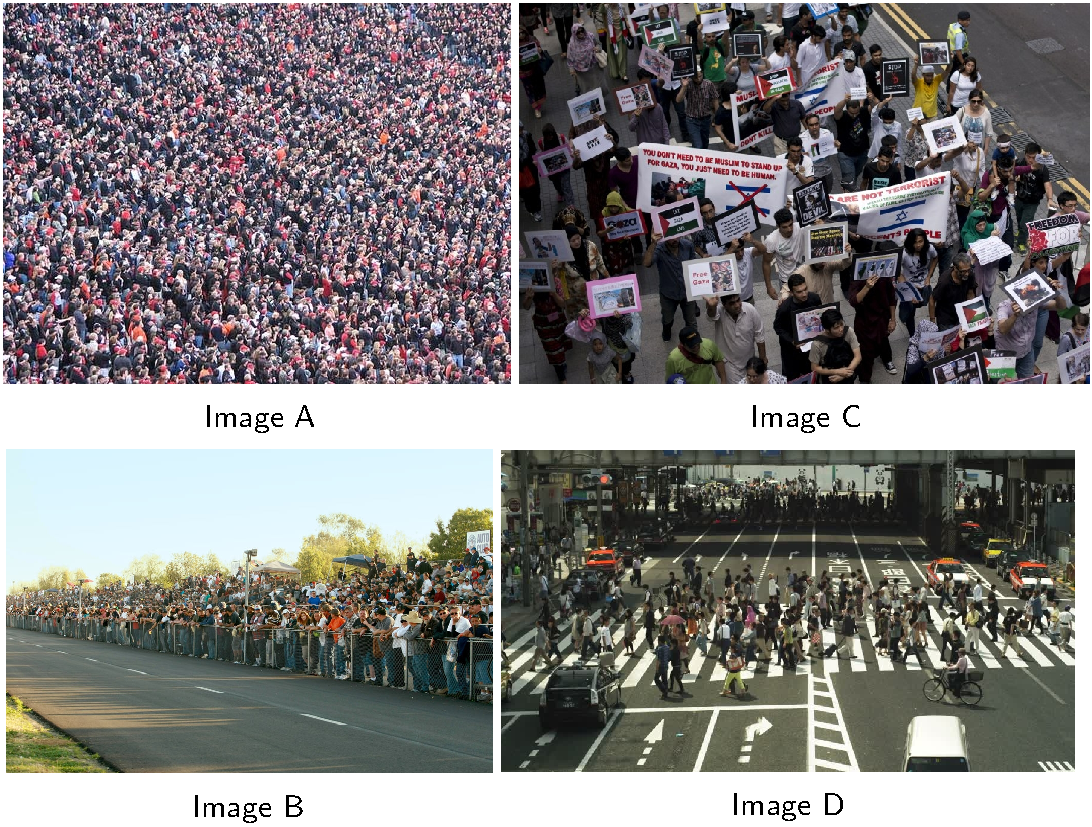
\includegraphics[scale=0.6]{figures/introduction_1.pdf}
		\caption{Different semantic interpretation for images figuring the semantic concept \emph{crowd}}
		\label{introduction_1}
	\end{figure}

	\section{Research Issues}
	%\addcontentsline{toc}{section}{Research Issues}
	%\sectionmark{Research Issues}
	Despite advanced \gls{IR} capabilities, user still unsatisfied by their delivered search results. This discontent 
	is caused commonly by \revAnglais{non-relevant} results that can be due to a \revAnglais{non-good} understanding of stored documents, 
	and/or the \revAnglais{non-apprehension} of the user query. In fact, popular and widely-used search engines, 
	like \textsc{Google}, \textsc{Bing} and \textsc{Yahoo !}, essentially rely on classical 
	keyword matching techniques, and their relevance is often unsatisfying owing to inaccurate 
	textural tag information.

	In such a situation, the multimedia retrieval community has looked for new approaches
	in order to make the availability of automated and efficient semantic interpretations for multimedia contents. 
	Thus, a number of diverse approaches for semantic multimedia content analysis have been proposed addressing 
	the discovery of multi-modal features \citep{Marques2012} like visual features (patterns, color, histograms, \dots{}) and
	audio features. In particular, Content based image retrieval 
	\gls{CBIR} has attracted \revAnglais{a lot of attention} over the last two decades 
	\citep{Rui1999,Smeulders2000,Datta2005,Liu2007,Huurnink2012}. 
	However, these earlier approaches failed to reduce the semantic gap between the extracted features and the 
	user's perception. Then, the next approaches focused on exploring these low-level features in order 
	to detect high level-feature (semantic objects and concepts) \citep{Datta2008,Snoek2008,Egozi2011}. 
	These semantic analysis based approaches proved to be highly effective and useful in many application 
	areas, but, once again, failed to deliver an efficient semantic interpretation \citep{Snoek2010,Over2013}.
	Under such a context, exploring further semantics within a multimedia content is a major challenge.

	To sum up, in our dissertation, we considered that a knowledge based approach should be more explored 
	and tackled. We addressed the following research issues:

	
	\begin{description}
		\item[Issue 1: A novel \revAnglais{knowledge} based approach for video/image indexing]
		other than low-level and high-level ones, further semantic information is gathered 
	from a multimedia content in order to better interpret a semantic content. Motivated by a kindred vision 
	of human perception, new approaches have investigated the engineering of knowledge-based approaches 
	for multimedia retrieval, in particular, the ontologies 
	\citep{Mylonas2008,Hudelot2008,Mylonas2009,Elleuch2011,Paliouras2011,Bannour2014}.
	Yet, ontologies \citep{Petridis2004,Wallace2005,Moeller2008,Dou2015}
	(as a knowledge database) are powerful tools to design concepts/contexts 	
	and their interrelationships. In general, ontology-based approaches 
	\revAnglais{consist} in defining a knowledge conceptualization and a reasoning process in order to handle and 
	enhance a semantic interpretation. However, these recent approaches 
	still facing some issues related to the construction of the ontology and the definition of its content.

		\item[Issue 2: dealing with uncertain knowledge and interpretations]
	Multimedia content interpretation and the user perception give evidence to the uncertain nature of the retrieval
	task which can benefit \revAnglais{from} either fuzzy or probabilistic approaches. In order to model uncertain and 
	imprecise knowledge for multimedia contents, many approaches were proposed. There are many discussions
	about these two approaches and their capabilities to handle and support uncertainty.
	In fact, endless arguments are defended by the knowledge extraction community about  the effectiveness 
	of fuzzy approaches and probabilistic ones \citep{Gaines1978,Bosko1990,Sanjaa2007,Zadeh2014,Zadeh2015}. 
	In this dissertation, we focused on the use of a fuzzy approach. Thus, the use of fuzzy 
	processing techniques to multimedia indexing and retrieval approaches has been extensively investigated 
	in literature. Mainly, fuzzy retrieval models offer more flexibility to handle indexing terms, query 
	terms and pertinent document ranking. The multimedia retrieval community took advantage by the use of 
	fuzzy theory based models for knowledge representation and management.

		\item[Issue 3: Scalability]
	Multimedia collections are increasing staggeringly. Thus, retrieving from large-scale datasets 
	is a challenging task \citep{Villegas2013,Villegas2014,Gilbert2015,Villegas2015}.
	The access to such an enormous \revAnglais{content} has forced the multimedia retrieval community to look for advanced scalable
	approaches and techniques in order to make the availability of automated and efficient semantic 
	annotation for such contents \citep{Wang2011,Zhang2012,Benavent2013,Sahbi2013,Reshma2014}.
	
	\end{description}
	

	Our present thesis work is part of the \textsc{i-Tv} project led by the \textsc{RegimVid} team. 
	The latter project \revAnglais{focuses} on an intelligent and personalized access to a video data system via 
	a complete process from low-level processing to viewing multimedia corpus. Our research works deal 
	with issues of semantic understanding and reasoning for video/image contents. 
	\revAnglais{In the dissertation, we particularly focus on} 
	how to better understand and interpret an uncertain semantic content efficiently through
	the use of fuzzy ontologies. Our approach is based on defining a fuzzy knowledge dataset in order to 
	enhance video/image semantic interpretation, and to overcome the scalability issue. 




%%%%%%%%%%%%%%%%%%%%%%%%%%%%%%%%%%%%%%%%%%%%%%%%%%%%%%%%%%%%%%%%%%%%%%%%%%%%%%%%%%%%%%%%%%%%
	

	\section{Aims and Contributions}
	%\addcontentsline{toc}{section}{Aims and Contributions}
	%\sectionmark{Aims and Contributions}
As aforementioned, the aims of this thesis are threefold. (1) At a first step, we have attempted to suggest a knowledge based model to enhance the indexing accuracy within a multimedia retrieval system. (2) Subsequently, we have concentrated our contributions on an effective use of the knowledge based model in order to improve multimedia content analysis and indexing. (3) Finally, we have concentrated our contributions on the scalability issue when handling large-scale multimedia data and a considerable amount of semantic of their contents.

The figure \ref{introduction_3} illustrates the general work-flow of the proposed approach for a knowledge based framework to enhance the indexing accuracy.


In this dissertation, we attempted to reach the following objectives:

\begin{description}
	\item[Objective 1 ($Obj_{1}$)] Dealing with a new knowledge based model for
		multimedia indexing. The objective is to develop a framework able to handle various information 
		about a multimedia content, then to operate with \revAnglais{this} information in order to infer new 
		information/knowledge through a reasoning process. Such a novel model has to define and highlight 
		pertinent components for an efficient knowledge based indexing process \citep{Zarka2011,Ksentini2012},
	\item[Objective 2 ($Obj_{2}$)] Handling a fuzzy knowledge 
		when reasoning with semantic interpretations in order to enhance and enrich them. This objective 
		aims to define a semantic structure to model required knowledge, then to specify an automated ontology 
		population from available annotated image/video datasets, and finally to handle ontology content evolving 
		to further improve semantics capabilities through \revAnglais{analyzing} and revising inaccurate and irrelevant
		knowledge \citep{Elleuch2011,Zarka2015},
	\item[Objective 3 ($Obj_{3}$)] Ensure the capability to handle a large-scale multimedia indexing 
		collection: the scalability
		While recent works focused on the use of semantic hierarchies to improve concept detector accuracy, 
		this objective embodies the use of such hierarchies to reduce detector complexity and then, to handle 
		efficiently large-scale datasets \citep{Zarka2015a}.
\end{description}


	Consequently, we denote that the outcomes of our thesis work will allow to address the following problems:
	\begin{itemize}
		\item Reducing the semantic gap through providing an effective knowledge based 
			framework for enhancing a semantic interpretation,
		\item Reducing the uncertainty through the use of fuzzy reasoning framework with 
			the aim of assessing the consistency of the indexing process,
		\item Ensuring the scalability aspect through handling hierarchical indexing process 
			which scales well with large-scale multimedia content.
	\end{itemize}

	\begin{figure}
		\centering
		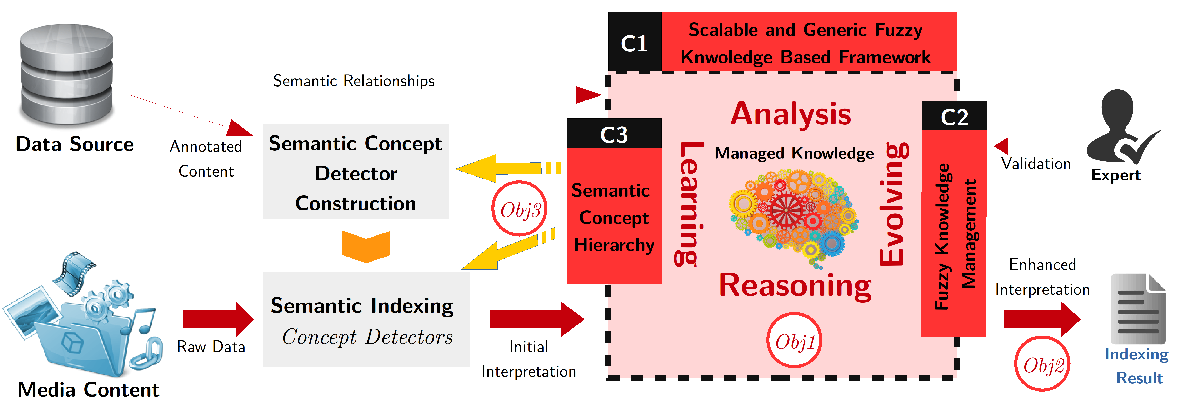
\includegraphics[scale=0.82]{figures/introduction__tmp.pdf}
		\caption{The proposed knowledge based framework: Handle a knowledge dataset to enhance the indexing process accuracy}
		\label{introduction_3}
	\end{figure}

	What was accomplished in our study is a novel ontology management which is intended to a machine-driven
	knowledge database construction. Such a method could enable semantic improvements in large-scale multimedia 
	content analysis and indexing. Thus, the main contributions for our thesis work are enumerated as follows 
	(see figure \ref{introduction_3}):
		\begin{description}
			\item[Contribution 1 ($C_ {1}$):] A fuzzy knowledge based framework for multimedia
				indexing to handle various interpretations about a video content. The framework 
				operates with these initial interpretations in order to infer enhanced interpretations 
				through a fuzzy reasoning process,
			\item[Contribution 2 ($C_ {2}$):] An automated and scalable fuzzy ontology management approach 
				(knowledge extraction, population, reasoning and evolving) for managing and 
				enhancing fuzzy interpretation about a video content,
			\item[Contribution 3 ($C_ {3}$):] A scalable ontology-driven approach to construct hierarchical 
				Semantic concept detectors. Fuzzy knowledge \revAnglais{is} used then at both learning and detection
				steps in order to enhance concept detectors accuracy, and to reduce the number of 
				semantic concepts to be picked up within a content.
		 \end{description}

	In order to illustrate the semantic enhancement of concept detection introduced by our proposed scalable 
	and generic ontology-based framework, the following section enumerates  different conducted experiments 
	within multimedia evaluation campaigns.

%%%%%%%%%%%%%%%%%%%%%%%%%%%%%%%%%%%%%%%%%%%%%%%%%%%%%%%%%%%%%%%%%%%%%%%%%%%%%%%%%%%%%%%%%%%%
	\section{Evaluation and Applications}
	%\addcontentsline{toc}{section}{Evaluation and Applications}
	%\sectionmark{Evaluation and Applications}
	In addition to the theoretical formulation of the proposed approach, we conducted some 
	empirical evaluations over large-scale realistic data sets in the general domains. 
	We first evaluated our approach within the standard benchmark 
	\textsc{\gls{TrecVid}} \citep{Smeaton2006,Smeaton2009,Over2014}. We also applied our 
	approach to real image data from different domains delivered by \textsc{Flickr} data 
	collections \citep{Wang2009}.

	Different evaluation metrics, including \emph{Mean Average Precision} (\gls{MAP})
	\citep{Schoeffmann2012}, \emph{Inferred Average Precision} (\gls{infAP}) \citep{Yilmaz2008} and 
	\emph{Geometric Mean Average Precision} (\gls{GMAP}) \citep{Thomee2012} are used in our experiments. 

	Our evaluations \revAnglais{also concern} the scalability issue. We handled a large scale video 
	dataset (about $8~000$ hours from \textsc{\gls{TrecVid}}) and a large-scale image dataset 
	(up to $500~000$ images from \textsc{Flickr}).

	Based on the proposed approaches and techniques, we participated to the development 
	of the \textsc{RegimVid} system \citep{Elleuch2010,Feki2012,Ksibi2013}:  
	a semantic video indexing, retrieval and visualization system.

	Our conducted experiments can be epitomized within these tasks:
	\begin{itemize}

		\item \textit{Semantic Video Indexing}: We first explored a multi-modal fuzzy fusion model 
		to handle different semantic interpretation gathered by various modalities (text, audio, visual, \dots{}).  
		A practical system was designed to incorporate the latter fusion model. We used the developed system 
		in order to enhance a video semantic indexing within the \emph{Semantic Indexing} task of the 
		\textsc{\gls{TrecVid}} 2010 \citep{Elleuch2010,Zarka2011,Over2011} evaluation campaign,


		\item \textit{Photo Annotation}: After exploring knowledge database capabilities for enhancing 
		a semantic interpretation, we proposed a fuzzy ontology based reasoning framework for managing valuable 
		knowledge in order to open up a semantic interpretation about a content. The proposed framework was 
		evaluated within the \emph{ImageCLEF2012's Flickr Photo Annotation and Retrieval} 
		\citep{Thomee2012,Zarka2015} evaluation campaign,

		\item \textit{Scalable Photo Annotation}: the aforementioned knowledge based framework being formulated 
		and evaluated, we investigated a study on the semantic indexing scalability issue through considering 
		an ontology based hierarchical image annotation. We evaluated, then, this framework within 
		\textit{ImageCLEF2015 Scalable Concept Image Annotation} \citep{Gilbert2015,Villegas2015,Zarka2015a} task.

	\end{itemize}

	\section{Thesis Overview}

	At this point, many questions have arisen: what is an appropriate model/approach to introduce the
	knowledge management in an indexing system? Then, how to profit from a knowledge database to enhance 
	the indexing accuracy? Finally, how to cope with the scalability issue? 

	Keeping in mind our chronological progression in achieving the enumerated above objectives and 
	contributions, the rest of the present dissertation is organized through three parts as follows:

	\begin{enumerate}
		\item \textit{\textbf{Part I - Video Indexing: Background and Trends}}
		\begin{itemize}
			\item \textbf{Chapter \ref{state1}:} introduces a general overview of the Multimedia Information Retrieval.
			It describes also the main proposed models, the common assessment measures and the methodologies.
			The chapter ends with an enumeration of actual video indexing issues and trends.
			
			\item \textbf{Chapter \ref{state2}:} introduces a survey of the use of fuzzy knowledge databases to solve problems 
			discussed in the previous chapter. After enumerating actual related works, we show a discussion 
			over the survey in order to motivate and introduce our proposed fuzzy ontology based model 
			for video indexing	
		\end{itemize}

		\item \textit{\textbf{Part II - Fuzzy Ontology Based Framework for Video Indexing}}
		\begin{itemize}
			\item \textbf{Chapter \ref{c1}:} displays a new approach for video indexing through the use of 
				fuzzy ontologies. Our approach takes advantages of the fuzzy knowledge in order 
				to enhance video indexing accuracy. Then, we focus on modelling and handling \revAnglais{this}
				fuzzy knowledge within an ontology. Therefore, an ontology management model is presented.

			\item \textbf{Chapter \ref{c2}:} proposes to go further in the use of fuzzy ontologies models for 
				enhancing video indexing accuracy. In particular, we address the following issues: 
				how to extract valuable fuzzy knowledge? How to model \revAnglais{this} fuzzy knowledge within
				an ontology? How to reason with \revAnglais{this} fuzzy knowledge in order to improve a semantic
				interpretation? And finally, how to evolve the extracted knowledge? Therefore, we propose 
				to \revAnglais{automatically construct} fuzzy ontologies to handle efficiently information about 
				a video content.

			\item \textbf{Chapter \ref{c3}:} explores the contribution of semantic hierarchies for image annotation 
				in order to handle the scalability issue. Thus, we propose an ontology driven hierarchical 
				image annotation owing to reduce the number \revAnglais{of semantic concepts} to be detected 
				within a content. 
		\end{itemize}

		\item \textit{\textbf{Part III - Conclusions and Future Research Directions}}
		\begin{itemize}
			\item \textbf{Chapter \ref{conlusion}:} states a feedback on our contributions and discusses
				future directions that can be tackled by the presented research topics.
		\end{itemize}
	\end{enumerate}

	

	\section{Publications}
	%\addcontentsline{toc}{section}{Publications}
	The aforementioned contributions in the fuzzy ontology based semantic enhancement for video 	
	indexing have been justified  by the following scientific publications:  
		\paragraph{International Journal}
			\begin{itemize}
				\item \textbf{Zarka, M.}, Ben Ammar, A., \&{} Alimi, A. (2016). 
				Fuzzy reasoning framework to improve semantic video interpretation. 
				\emph{Multimedia Tools and Applications}, $75$(10), 5719–5750. \\Retrieved from 
				\texttt{http://dx.doi.org/10.1007/s11042-015-2537-1}
				\\doi: \texttt{10.1007/s11042-015-2537-1}
			\end{itemize}

		\paragraph{International Peer-Reviewed Communications}
			\begin{itemize}
				\item \textbf{Zarka, M.}, Ammar, A. B., \&{} Alimi, A. M. (2011). 
				Multimodal fuzzy fusion system for semantic video indexing. 
				In \emph{IEEE symposium on computational intelligence for multimedia,
				signal and vision processing, CIMSIVP 2011, Paris, France} (pp. 60--66). IEEE.

				\item Elleuch, N., \textbf{Zarka, M.}, Ammar, A. B., \&{} Alimi, A. M. (2011). 
				A fuzzy ontology: Based framework for reasoning in visual video content analysis 
				and indexing. In Proceedings of the eleventh international 
				workshop on multimedia data mining (pp. 1--8). New York, NY, USA: ACM. \\
				Retrieved from \texttt{http://doi.acm.org/10.1145/2237827.2237828}\\
				doi: \texttt{10.1145/2237827.2237828}

				\item Ksentini, N., \textbf{Zarka, M.}, Ammar, A. B., \&{} Alimi, A. M. (2012). 
				Toward an assisted context based collaborative annotation. In P. Lambert (Ed.), 
				\emph{10th international workshop on content-based multimedia indexing, 
				CBMI 2012, Annecy, France, June 27--29, 2012} (pp. 71--76). IEEE.\\
				Retrieved from \texttt{http://dx.doi.org/10.1109/CBMI.2012.6269852}\\
				doi: \texttt{10.1109/CBMI.2012.6269852}
			\end{itemize}
		\paragraph{International Benchmarks}
			\begin{itemize}
				\item Elleuch, N., \textbf{Zarka, M.}, Feki, I., Ammar, A. B., 
				\&{} Alimi, A. M. (2010). REGIMVID at TRECVID2010: semantic 
				indexing. In P. Over et al. (Eds.), \emph{TRECVID 2010 workshop
				participants notebook papers, Gaithersburg, MD, USA, November 2010}. 
				National Institute of Standards and Technology (NIST). \\
				Retrieved from \\\texttt{http://www-nlpir.nist.gov/projects/tvpubs/tv10.papers/regim.pdf}

				\item \textbf{Zarka, M.}, Ben Ammar, A., \&{} Alimi, A. (2015). 
				Regimvid at imageclef 2015 scalable concept image annotation 
				task: Ontology based hierarchical image annotation. 
				In \emph{Working notes for CLEF 2015 conference , 
				Toulouse, France, September 8--11, 2015.}
			\end{itemize}



	\regimfancy
	\part{Video Indexing: Background and Trends}
			\chapter{Multimedia Information Retrieval and Indexing}
\label{state1}
	
	The Information Retrieval aims to define approaches and techniques to model, store and 
	access information items \citep{Baeza-Yates2011}.
	The information can take different forms: textual document, an audio sequence, a visual 
	data (images) or a video clip. Thus, the multimedia information retrieval 
	field engages many research areas as signal processing, 
	machine learning, data mining, information theory, human-computer interaction and many other 
	areas \citep{Rueger2010,Sheu2010}. Many researches \revAnglais{have} addressed an important interest to multimedia 
	information retrieval in recent years. In fact, the raising of advanced multimedia devices 
	together with the low cost storage devices have blown-up the production and the 
	access to multimedia data content.

	The present chapter describes basic concepts of multimedia retrieval and indexing which consist of the 
	general architecture and the evolution of retrieval approaches from the text-based toward the concept-based 
	approach. This chapter ends with an enumeration of open issues in semantic video indexing.

	\section{Multimedia Information}

	%In figure \ref{state_fig1}, the information side contains a large amount of multimedia content that the 
	%Information System has to process, analyze and manage. 
	The multimedia content formats can vary 
	according to the usage domain, for example web pages, video sequences, audio sequences, \dots{}. 
	All these broadly different \revAnglais{understandings} of what a multimedia content \revAnglais{help} to interpret the 
	semantics within a defined content. In fact, for a given multimedia content, we can identify different
	basic data types (such as text, image, video, speech, audio), interactive elements 
	(links, event on user action, mouse over, \dots{}) and structural elements (text formatting, image and 
	video location, \dots{}). The syntax of a multimedia content is a collection of several different  data 
	types that provide rich information and enhanced experience for the reader \citep{Stamou2005}.

	As depicted in figures \ref{state_fig2} and  \ref{state_fig3}, we conclude that humans segment a multimedia 
	document into manageable blocks of information in order to construct a complete understanding of 
	that content. Thus, in this thesis, we consider a multimedia content as an image and audio stream 
	that carry some semantic information. The figure \ref{state_fig3} illustrates a scene of car racing. 
	While the first segment depicts some racing cars, the second segment depicts aligned cars at the start 
	line. By identifying valuable objects and sounds within that content, we aim to generate a more 
	complete and enhanced semantic interpretation. Video segmentation, visual objects detection and audio 
	analysis are discussed in two other thesis works \citep{Feki2013,Elleuch2015a} 
	carried out jointly with the present one.

	\begin{figure}[ht]
		\centering
		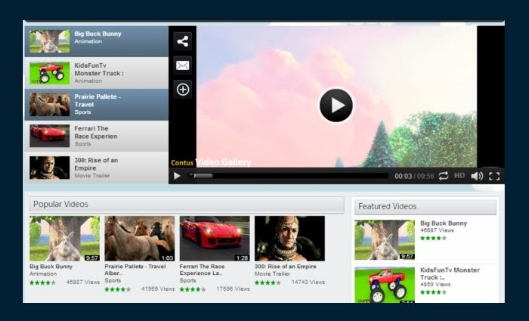
\includegraphics[scale=0.8]{figures/state_fig3}
		\caption{A Web page can be seen as a multimedia document}
		\label{state_fig2}
	\end{figure}

	\begin{figure}[ht]
		\centering
		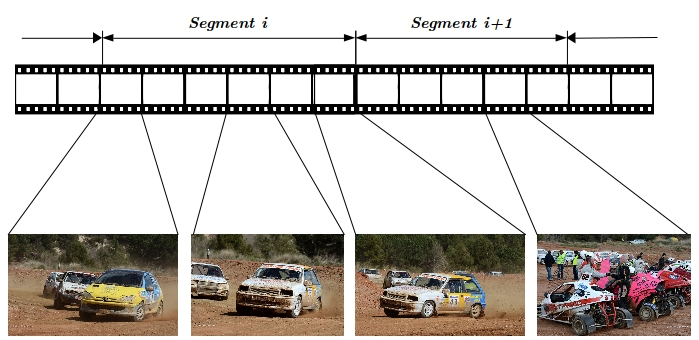
\includegraphics[scale=0.7]{figures/state_fig4}
		\caption{Video sequences can be seen as a multimedia document}
		\label{state_fig3}
	\end{figure}

	%In the figure \ref{state_fig1}, the user side displays a generic paradigm of Information retrieval: 
	%the user defines some information need, and the system supplies the required information. 

	Unlike textual documents, a multimedia content contains more than symbols that a user can take on 
	in order to express his need for information. At first, the multimedia content is rich in term 
	of available semantic information: the visual content can expose a variety of messages and emotions, 
	an audio content can also expose feeling and emotions, then, the structure itself 
	(spatial-temporal information) also communicates valuable information. Thus, a multimedia content 
	delivers a complete semantic interpretation to be communicated to the user. Secondly, the computational 
	system can process only mathematical and logic expressions, and not all what a human can express 
	and interpret in term of ideas, emotions and feeling: the communication gap between the user and the system.

	Many approaches were proposed in literature in order to empower the user with tools to express 
	his query and achieve a better mapping between the expressed user need, the extracted 
	multimedia information, and what the system can  successfully match. Some of these techniques 
	will be exposed in the following sections.

	\section{Multimedia Information Retrieval}

	In order to access a multimedia content, some techniques are used to interpret a
	human queries that translate its needs, and then to retrieve the closest match. 
	As an example, a user searches its collection using the keyword or a phrase such 
	as \emph{car} or \emph{car racing}, he will expect the information retrieval system 
	to return all relevant items. Nevertheless, the user still disappointed with the given 
	results. Such a disappointment can be rooted in two reasons. Firstly, the context in 
	which the user has expressed its information need could be too vague and requires the user
	to further refine its query. Secondly, the weak and blurred link between the information
	representation schemes and the user semantic query. These two issues are called the
	\emph{semantic gap} \citep{Smeulders2000,Bahmanyar2015}.

	Low-level extraction approaches from visual contents (e.g., histograms, shapes, motions, \dots)
	and audio content (e.g. volume, frequency, pitch, …) are widely investigated, providing a wide 
	feature sets that could be explored for indexing and modeling a multimedia content. These low-level 
	features rely on data-driven properties and characteristics, which may be misrelated to the concepts 
	expressed in the semantic query.

	The semantic information extraction process from multimedia contents is considered as an artificial 
	intelligence problem. Nevertheless, Human perception is still being not well understood for imitating 
	it in a computational system. In fact, an Information Retrieval (IR) system \revAnglais{is} considered as an 
	artificial intelligence problem, on one hand, because the system has to mimic the human perception 
	process in order to extract relevant semantics from a given multimedia content, and on the other hand, 
	the system has to interpret the user query and match the relevant stored information. 
	Then, the missing relationship between low-level features and human knowledge is the fundamental semantic 
	gap problem when we need to search a multimedia collection by expressing some semantic queries. 
	
	Recent proposed multimedia analysis and indexing approaches rely mainly on manual annotations 
	\citep{Wang2011,Lazaridis2013,Jin2015}. Such approaches are flawed and costly, and can lead to 
	a poor learning process.  As depicted in figure \ref{state_fig1}, the user query is analyzed by the information 
	retrieval system with the same system that can imitate human perception in order to process the query 
	and match it to relevant information. The semantic gap exists in both: (1) multimedia content analysis, 
	and (2) user query understanding.

	In this scope, actual researches in multimedia retrieval are exploring new paradigms for semantic 
	multimedia information analysis in order to deliver a higher degree for semantic information 
	processing capabilities. In fact, the multimedia community addressed more intention on knowledge 
	management based approaches for such a propose. 

	\begin{figure}[ht!]
		\centering
		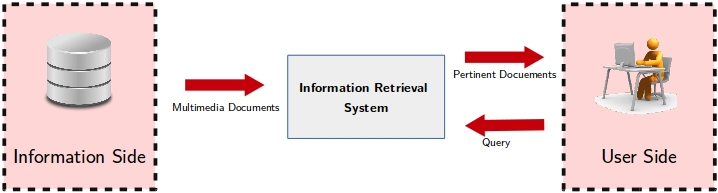
\includegraphics[scale=0.8]{figures/state_fig1}
		\caption{Information work-flow in Information Retrieval}
		\label{state_fig1}
	\end{figure}

	%Before discussing the ontology based approaches,
	We will continue, in the following, 
	to display and identify the information retrieval main research directions. 

	The information system has been proposed since several decades. Most of proposed systems
	until mid $90^{s}$ handled only text data based documents \citep{Manning2008,Marcia2012}.
	 From such an experience, a set of functional components were \revAnglais{defined:}
	(1) the analysis component that extracts a vocabulary from documents, 
	(2) The indexing module that represents documents through its information symbols, 
	(3) the query processing component that transforms a user information needs into information symbols, and 
	(4) the retrieval component that ranks the stored documents representation according to the similarity 
	measure between information symbols.

	A multimedia information system, as displayed in figure \ref{state_fig4}, is similar to the traditional 
	Information retrieval system detailed above, but with different algorithms: the multimedia analysis handles 
	multimedia content unlike a text document. Thus, the information retrieval system architecture depicted in 
	figure \ref{state_fig4} can be addressed as a generic information retrieval system. In the \revAnglais{following}, we detail 
	the components of this generic architecture.

	\begin{figure}[ht]
		\centering
		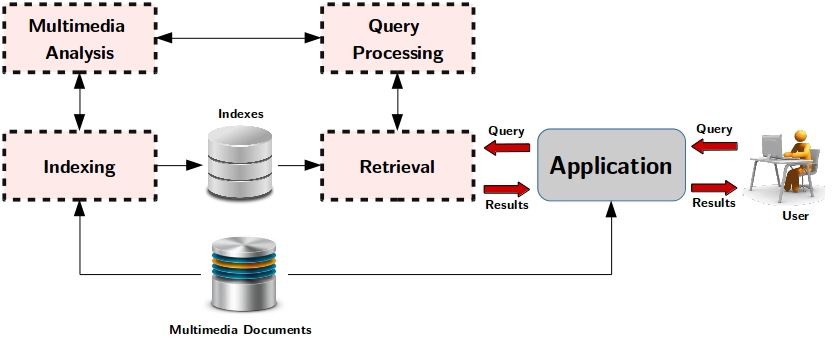
\includegraphics[scale=0.7]{figures/state_fig2}
		\caption{Classic Multimedia Information Retrieval Architecture}
		\label{state_fig4}
	\end{figure}

		\subsection{Multimedia Analysis}	

		Information Retrieval systems \revAnglais{analyze} multimedia contents and extract features measuring 
		the importance of information symbols. The extraction of these features aims: 
		(1) to associate multimedia contents to meaningful symbols of information that 
		a user can use to search for, and (2) to quickly find relevant document through
		information symbols indexing.

		These information symbols re-extracted automatically, semi-automatically or manually 
		\citep{Zhang2012}. While the automatic information symbols extraction executes an analysis 
		task without a human intervention, the semi-automatic one includes a human as part of the analysis
		task: some information can only be detected and added by a human, such as the name of a person, 
		or the relation between two persons (e.g. friends). Many approaches were proposed, but more adequate
		to the considered information domain. As an example, \textsc{Google} \citep{Chen2011,Kumar2014}
		and \textsc{Flickr} \citep{Sigurbjoernsson2008,Ginsca2014} page rank rely on some human
		intervention in order to edit information, and then improve search results. While \textsc{Flickr} 
		allows the user to tag images with a set of keywords that can be used later for searching images, 
		\textsc{Google} \revAnglais{relies} on human edited links pointing to analyzed web pages in order to adjust its 
		importance. We conclude that \textsc{Flickr} adopts a semi-automatic approach, and \textsc{Google}
		adopts an automatic one since it relies on stored information.

		\begin{figure}[ht]
			\centering
			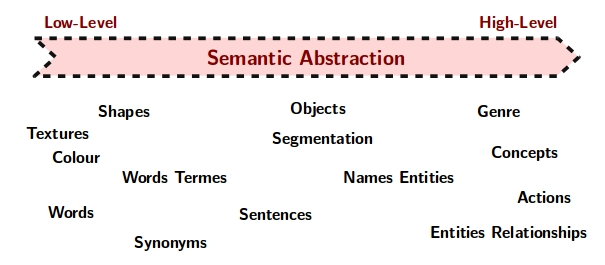
\includegraphics[scale=0.7]{figures/state_fig5}
			\caption{Relation between information symbols and semantic abstraction}
			\label{state_fig5}
		\end{figure}

		The figure \ref{state_fig5} displays some feature \revAnglais{positions on} a semantic abstraction level: 
		from low-level features to high-level ones.  While low-level features, such as color histogram,
		are easily extracted from a multimedia content through automatic methods, high-level features, 
		such as content topic or objects existing in the content, require more complex approaches
		due to the high semantic dimension that they involve.

		Classical text analysis approaches produced a small set of features (e.g. occurring words). 
		However, multimedia analysis approaches generate scores, such as a probability, for all 
		possible features (information symbols). Such a situation will induce to produce dense 
		high-dimensional vectors that contain all features extracted from all multimedia documents, 
		and then cause several issues such as storage space. Thereby, the multimedia analysis approaches
		\revAnglais{are} important since they will impact the entire multimedia \revAnglais{information} system. 
		So, many techniques and algorithms are provided to \revAnglais{dress} these issues.
		
		\begin{itemize}
			\item \textit{Low-Level Analysis: }
				The low-level analysis extracts features from a multimedia content. 
				These features are commonly related to human senses or language (e.g. image colors,
				image textures, audio rhythms, word, \dots{}). Such features are well studied in
				literature and most of them have been developed in the area of data compression 
				that exploits the characteristics of human vision and hearing senses 
				\citep{Foerstner1994,Nixon2012}. 

				These low-level features are used then to index multimedia contents.

			\item \textit{High-Level Analysis: }
				The High-level analysis aims to extract inferred information from a multimedia content. 
				\revAnglais{This} extracted information can be not explicitly detectable by a computer. 
				Then, a prior-knowledge about the problem domain semantics should be involved. 
				Such domain centered knowledge \revAnglais{is} formally described by a set of semantic concepts
				identified by keywords. The latter capture part of domain knowledge which can be used
				to detect the presence of a concept in a given multimedia content. 

				The high-level features (concept/keyword) are used as index tokens that the 
				information retrieval system uses to build the index of a semantic-multimedia content.
		\end{itemize}

		\subsection{Indexing}

		Information features (symbols) extracted from a multimedia content  are stored by the indexing
		component. While the analysis component impacts the effectiveness of the multimedia information 
		system, the indexing one impacts the efficiency of the system. The main aim of the indexing algorithm 
		is to manipulate an inverted-file index that enumerates all information symbols and all 
		related documents that \revAnglais{contain} these symbols.

		The indexing component uses a high-dimensional index to accommodate the high-dimensional 
		multimedia content data nature (as the multimedia analysis component produces a score for 
		all possible feature type and dimension). The efficiency of high-dimensional indexes \revAnglais{is} 
		related to several aspects \citep{Ai2013}: tree-structured indexes, hash-based indexes, compression of the
		index to reduce memory usage,  \dots{}. All these techniques allow a \revAnglais{more} faster and efficient
		look-up of the index table. In \citep{Baeza-Yates1999,Baeza-Yates2011}, the authors discussed 
		the efficiency of the indexing component.


		\subsection{Query Processing}

		When the user communicates query to the information retrieval system, the latter analyses and 
		transforms the query into an internal representation that used the same symbols for indexing
		multimedia contents. 

		The query processing component parses the user query according to a specific language,
		extracts information symbols and features, and proceeds it to the retrieval component 
		to search index for the matching documents.
		
		Text based information retrieval systems \revAnglais{handle} text queries as a query language support. 
		In multimedia information systems, the queries can be expressed in many ways \citep{Liu2007,Yasmin2014}. 
		In what follows, a brief enumeration of some of these queries methods.
		
		\begin{itemize}
			\item \textit{Sketch Retrieval:} this is one of the first proposed methods to query 
			a multimedia database \citep{Cao2010,Cao2011}. The user query is in the form of a visual
			sketch of what the user \revAnglais{expects} to find. The information retrieval system proceeds then the 
			extraction of features from that sketch in order to search the index for images that are 
			visually similar.
			
			\item \textit{Search by Example:} the user can submit an example image representing the 
			information he \revAnglais{is} searching for. In such a case, the query processing extracts the low-level 
			features for the query in order to look for similar stored documents with similar features.
			
			\item \textit{Search by Keyword:} this is by far the most popular search query method: 
			the user describes his information request with a set of keywords. \revAnglais{Then}, the system
			searches for multimedia content that corresponds to these keywords. The issue of this 
			high-level query method is that the user can only use some predefined keyword vocabulary 
			used also in multimedia content indexes.
			
			\item \textit{Personalized/Adaptive Retrieval:} this is a refinement to all other search methods. 
			It explores the history and profile of the user search \citep{Magalhaes2004}. 
			\revAnglais{This} extra-information can enhance the search experience by filtering information
			to particular domains, limiting certain document formats, \dots{}.

		\end{itemize}

		\subsection{Retrieval}

		The retrieval component computes indexed document ranks according to their similarities to a user query. 
		This component browses and sweeps the index according to the input query information symbols to 
		search for most similar documents according to the relevance degree. The latter is computed by a 
		function that determines the semantic relatedness degree between the query and the retrieved documents. 
		Thus, the result delivered by the retrieval component is a set of ordered documents that \revAnglais{are} judged 
		as similar documents to the given query \citep{Memar2013}. 

		The challenging problem in the ranking task is to find which documents are relevant and which
		are irrelevant. The relevance degree between the document and the user query is computed through
		various retrieval models. The information retrieval community proposed different retrieval models
		\citep{Baeza-Yates1999,Croft2010} such as: Boolean, vectorial, probabilistic and fuzzy models.

		\begin{itemize}
			\item \textit{Boolean Model:} is the oldest and the classical retrieval model. 
			It is based on the Boolean algebra. With such a model, a query is defined 
			as a Boolean expression, and the relevance of a document  to a query is computed by the 
			use of Boolean operators like \emph{And}, \emph{NOT} and \emph{OR}. One limitation of 
			the boolean model is that computed relevance weights are equal for all relevant documents: 
			it will be difficult then to identify the most relevant documents between the less ones.
	
			\item \textit{Vector Space Model:} is the most popular and used retrieval model. 
			Both queries and documents are handled as vectors in the space. Then, the 
			similarity between a query and a document is estimated by the use of direction 
			and distance \citep{Manning2008}. 

			\item \textit{Probabilistic Model:} is a model that ranks document according to the 
			probability of relevance to a given query. This model uses the probability ranking 
			principal detailed in \citep{Fuhr1992}. Thus, a statistical distribution is used in order 
			to measure the relevancy between relevant documents and irrelevant ones.

			\item \textit{Fuzzy model: } Fuzzy logic plays an important role in many domains that handle 
			imprecise and vague information \citep{Mantaras2015}, such as text-mining, multimedia 
			information system, machine learning, \dots{}. To handle uncertain information, 
			the fuzzy logic allows intermediate truth values to be defined between 
			conventional evaluations of true (1) and false (0). Fuzzy logic was used as a fuzzy 
			retrieval model \citep{Tahani1976,Cross1994,Miyamoto2012}.
		\end{itemize}

	\section{Multimedia Retrieval Systems Evaluation}
		Information Retrieval has been widely addressed in research work, and it has been shown  
		to be highly useful to compare different systems and approaches. In literature, two different 
		measures are used: Firstly, an effectiveness metric is used to measure how well the system
		can satisfy the user information need. Secondly, the efficiency metrics measures both, 
		the system  responsiveness to the user query, and the system ability to cope with large-scale situations.
		
		Effectiveness and efficiency measures are widely affected by the data that is used to test a system. 
		In fact, a dataset can contain information with different complexities. Therefore, evaluation 
		methodologies are now being investigated and standardized. In the following, we enumerate 
		traditional metrics and resources used in the evaluation of information retrieval systems.

		\subsection{Effectiveness Evaluation}
		In order to introduce the retrieval effectiveness measure, we discuss the meaning of relevance.
		The relevance is a fundamental concept of information retrieval. The paper \citep{Mizzaro1997}
		is considered as the first work that focused on the relevance concept: \emph{the relevance is 
		claimed as a complex concept involving different aspects: methodological foundations, different 
		types of relevance, beyond-topical criteria adopted by users, modes of expression of the relevance 
		judgment, dynamic nature of relevance, types of document representation, and agreement among 
		different judges}.

		Therefore, many research areas adopt their own definition of relevance focusing more \revAnglais{on} their 
		specific objectives: the information retrieval aims to identify documents that can be judged as  
		the best answer to a given information query. Information retrieval relies on document datasets 
		where their relevance of a given query was judged by a human. Nevertheless, there is no general 
		definition of what a relevant document is. In fact, the relevance of  document is a diffuse 
		information because a given document can have different meanings to different humans. 
		This issue was widely discussed in literature that noticed a divergence between relevance 
		judgment made by different human for a given document \citep{Voorhees2000,Volkmer2007}.
		This divergence is more observable in large multimedia datasets. In fact, a multimedia content 
		is by nature subject of different interpretations and relevance annotation (judgment), also, 
		human relevance judgment process is a very costly task and large-scale document datasets will
		be partially annotated (incomplete and inconsistent).

		\emph{Precision} and \emph{recall} \citep{Buckland1994} are the popular information retrieval metrics. They are applied 
		on a ranked list of both relevant and non-relevant documents for a given query. While the precision 
		addresses the accuracy of the evaluated system, the recall addresses the completeness aspect.
		We enumerate, in the following, these two metrics and other derived ones.

		\begin{itemize}
			\item \textit{\textbf{Precision (Prec):}} which measures the ability of a
			system to present only relevant items. Mathematically, the Precision (\emph{Prec})
			is defined as the number of true positive documents ($T_{p}$) over the number of 
			true positives plus the number of false positives ($F_{p}$).
			\begin{equation}
				Prec = \frac{T_{p}}{T_{p} + F_{p}}
			\end{equation}

			\item \textit{\textbf{Recall (Rec):}} which measures the ability of a system
			to present all relevant documents.  Mathematically, the Recall (\emph{Rec}) is defined 
			as the number of true \revAnglais{positive documents} ($T_{p}$) over the number of true positives 
			plus the number of false \revAnglais{negative} documents($F_{n}$).
			\begin{equation}
				Rec =  \frac{T_{p}}{T_{p} + F_{n}}
			\end{equation}

			\item \textit{\textbf{F-measure (Harmonic mean):}} is a measure which assesses the
			trade-off between precision and recall. The \emph{F-measure} is computed as follows:
			\begin{equation}
				F =  \frac{2}{\frac{1}{Prec} + \frac{1}{Rec}}
			\end{equation}

			\item \textit{\textbf{Average Precision (AP):}} is obtained after each relevant 
			document is retrieved. Let $k$  be the number of relevant retrieved documents, the average 
			precision expression is:
			\begin{equation}
				AP = \frac{\sum\limits_{k\in \{r|r \text{ is rank of relevant docs}\}} 
					Prec@k}{\text{Number of relevant Documents}}
			\end{equation}

			\item \textit{\textbf{Mean Average Precision (MAP):}} is a metric which summarizes the
			overall system retrieval effectiveness into a single value as the mean of all 
			keywords average precision,
			\begin{equation}	
				MAP =  \frac{1}{|Q|} \sum_{q \in Q} AP_{q} \text{~~~~~where $Q$ is a set of queries}
			\end{equation}
		\end{itemize}
		These metrics measure the effectiveness of a given system in  fixed evaluation scenario. 
		Thus, the obtained measures are valid only for a specific scenario and \revAnglais{cannot} be generalized 
		to other situations.			

		\subsection{Efficiency Evaluation}

		The efficiency measurement in multimedia information system concerns the extra computational
		complexity over conventional information retrieval systems. This extra complexity is due to 
		the extra processing required to analyze a multimedia content and extract the contained 
		semantics.

		In the context of our thesis, we solely focus on the runtime complexity of the analysis component. 
		In fact, and as discussed in previous sections, the information indexing involves the indexing and 
		the storage of extracted low-level and high level features. The efficiency of the indexing task 
		measures both:
		\begin{itemize}
			\item \textit{Time complexity:} which measures how many documents/concepts per second 
			can the indexing task processes. Thus, the time complexity measures the system responsiveness.

			\item \textit{Space complexity:} which measures the amount of memory required to process a document 
			for the entire vocabulary. The space complexity measures the scalability aspect.
		\end{itemize}
		These two complexities define how well a system scales with several simultaneous requests.


		\subsection{Collections}

		In the assessment of semantic multimedia retrieval systems, multimedia collections 
		are used as research tools that provide a common test environment in order to evaluate and 
		compare different approaches and techniques. 

		Collections are used to evaluate a variety of techniques, such as shot-boundary detection, 
		low-level visual features, story segmentation, \dots{}. In this thesis, we address the problem of 
		indexing multimedia content by their semantic content. One aspect is required to be present in a 
		collection that will be used for the assessment of multimedia indexing: keywords that correspond 
		to concepts present in the collection content. They describe what meaningful concepts are present 
		within a given multimedia content.
	
		Multiple benchmarking initiatives have been proposed which aim the assessment of multimedia 
		retrieval system performances with \revAnglais{standardized} test collections and tasks, such as in 
		\textsc{ImageClef} \citep{Villegas2013,Villegas2014,Villegas2015} and \textsc{TrecVid} 
		\citep{Smeaton2006,Over2013,Over2014}. In what follows, we \revAnglais{enumerate} the multimedia 
		collections/benchmarks addressed in this thesis work.

		\begin{enumerate}
			\item \textit{\textbf{\textsc{ImageClef:}}} \textsc{ImageClef} is an evaluation forum for the 
			cross-language image retrieval.  The main goal of that benchmark is to provide the 
			required infrastructure for the evaluation of visual information retrieval systems 
			operating in monolingual, cross-language and language-independent contexts. 
			Thus, \textsc{ImageClef} allows  multilingual users accessing the growing visual 
			multimedia data, and creates a public resources for benchmarking information retrieval 
			systems and approaches. 

			Since its start in 2003, \textsc{ImageClef} \revAnglais{has been}
			a track in the \emph{Cross Language Evaluation Forum} 
			(\textsc{Clef}). The latter is one of the major forums for research in information retrieval. 
			The main goal is to create collections and topics in order to offer to the information retrieval 
			community an opportunity to evaluate and to compare theirs approaches.

			At first, \textsc{ImageClef} focused on text-based image retrieval. But since 2003, 
			the focus has shifted towards combining visual and textual features for multi-modal 
			image retrieval on general images collections, in particular medical ones.

			\textsc{ImageClef} is addressing the barriers between research interests and real-world 
			requirement by offering application-driven evaluation tasks. One of \revAnglais{these} tasks that 
			this thesis focused on is the \emph{Photo annotation} one.

			In \textsc{ImageClef 2012}, a collection of $25~000$ images was provided: 
			$15~000$ images for the development, and $10~000$ image for the test. The development dataset 
			was manually labeled with $94$ semantic concepts. But in \textsc{ImageClef 2015}, the collection has shifted 
			to $500~000$ and $240$ concepts, but with a very small development dataset (about $1~500$ images). 

			\item \textit{\textbf{\textsc{TrecVid:}}} Toward an efficient and effective management 
			of multimedia collections, many research works interest arising focusing on the combination 
			of multimedia interpretation, extraction, retrieval and management. This growing requirement 
			has initially resulted in the creation of a video retrieval track \textsc{TrecVid} within the 
			\textsc{Trec} conference. Actually, the \textsc{TrecVid} becomes a workshop in its own right.

			Founded in 2003, the \textsc{TrecVid} aims to promote and encourage research works in 
			content-based video retrieval and indexing through providing large test collections, 
			realistic system tasks, uniform procedures, and a forum for different researchers to 
			compare their results.

			\textsc{TrecVid} provides a several number of tasks, and in this thesis work, \revAnglais{we} focused 
			on the \emph{semantic indexing task}. The latter provides a collection of $400$ hours of 
			video sequences: $200$ hours for the development dataset, and another $200$ hours for the test one. 
			In 2010, \textsc{TrecVid} defined 130 semantic concepts, and in 2015, it defined 500 concepts.

		\end{enumerate}


	\section{Open Issues in Semantic Multimedia Retrieval}

	In the past few years, remarkable advances have been done relatively 
	to the video indexing at low-level as at high and semantic levels. Nevertheless, many open research 
	issues still be open and need to be more addressed in order to make an efficient use of video retrieval 
	systems \citep{Hole2015,Tunga2015}. In what follows, we identify some open challenges.

	\begin{description}
		\item[High-Dimensional Indexing] 
		The dimensions of extracted feature vectors used in most indexing systems to represent 
		video contents, are quite high (1024 dimensions in \citep{Elleuch2015}). There is a practical 
		requirement to reduce the intrinsic dimension of these feature vectors.
	
		\item[Similarity Matching] 
		The matching process within video retrieval requires similarity measurement for evaluation 
		feature vectors similarities. Classical retrieval systems use \emph{Euclidean} and \emph{cosine} 
		distance measure which fails to successfully simulate human perception similarity for a video content 
		\citep{Juneja2015}. Some similarity functions have been proposed in literature \citep{Shen2011}.
		%The matching process within video retrieval requires similarity measurement for evaluation feature 
		%vectors similarities. Classical retrieval systems use \emph{Euclidean} and \emph{cosine} distance
		%measure which fails to successfully simulate human perception similarity for a video content \citep{Juneja2015}. 
		%Some similarity functions have been proposed in literature \citep{Shen2011}. 
		Fuzzy similarities functions 
		enable more accurate similarity measurement \citep{Chen2002,Chaira2005,Baccour2013,Baccour2014,Kraft2015}, 
		but \revAnglais{fail} to deliver fast retrieval and to guarantee a better scalability \citep{Shen2011}.
		
		\item[Relevance feedback]
		First video retrieval systems were focused on fully automatic processing, 
		but they were unable to really produce promising and satisfactory results. 
		One of the occurred issues was the fact that user satisfactions of given results 
		were not taken into consideration. Thus, these systems included the use feedback 
		in order to learn from the user intervention and, then, to regulate the system process 
		for generating more satisfactory results. The relevance feedback can either be taken from the
		user directly, or it can come from intelligent approaches that capture and trace the user trends and profile.
		
		\item[Low-level/high-level semantic gap]
		Many of signal processing and computer vision contributions have been mostly explored in literature 
		for enhancing the video indexing and retrieval accuracy \citep{Brunelli1999,Liu2007}.
		More recent research works were focused on the high-level description and retrieval. 
		Actually, research works that bridge the semantic gap between signals (as an example: 
		pixels for images and frequency for audio) and implicit semantic information are taking 
		a growing interest. Knowledge management and reasoning are really taking more intention 
		and are opening many semantic barriers.
		
		\item[Performance Evaluation and Standard]
		Video indexing and retrieval is an area which highly requires standardization and uniform
		evaluation criteria in order to judge how well the system is performing and how it 
		performs better than other systems. Many evaluation campaigns (like \textsc{TrecVid} 
		\citep{Smeaton2006,Over2013,Over2014} and \textit{ImageClef} 
		\citep{Villegas2013,Villegas2014,Villegas2015}) proposed both development 
		and test dataset, and precision and recall based metrics.
		
		\item[Generic and multi-modal approaches]
		Expected video indexing and retrieval systems have to handle information and video contents 
		from different fields and disciplines. Moreover, they should take into consideration and analyze 
		all information from all the available modality of a given content (text, visual, audio, \dots{}). 
		Video information retrieval field is compelled to integrate  multi-modal signal processing, computer 
		vision,  Artificial Intelligence, knowledge management, \dots{}.

		\item[Scalable Indexing and Retrieval] 
		The high dimensions of the extracted features from a video content, and the contained rich 
		semantics represent massive data to be handled and computed. Efficient and scalable video 
		indexing and retrieval systems have to avoid overwhelming tasks. Scalable indexing and 
		retrieval techniques have to handle non overwhelming algorithms and tasks. 
		Thus, Scalable systems should ensure that the computing cost does not scale exponentially 
		with the amount of video data content and the semantics to be handled. 

		In spite of many research efforts to compact video extracted features \citep{Douze2010,
		Baroffio2013,Wang2015a,Li2015}, and to
		propose scalable indexing and retrieval techniques and approaches \citep{Caputo2014,Gilbert2015}, real scalable
		information retrieval systems still far from concretization.
	\end{description}

	\section{Conclusion}

	As denoted above, the multimedia retrieval community is tackling more robust indexing systems 
	in terms of effectiveness (that concerns in term of high semantic capabilities) and efficiency
	(that concerns the scalability and high-dimensional indexing abilities). In the chapter, 
	we show how the knowledge based approaches are considered as compelling direction to overcome
	the above issues.

			\chapter{Video Indexing: From signal processing to knowledge reasoning}
\label{state2}

Since multimedia resources are playing an increasingly outstanding role in our lives, the previous two decades have marked a great move 
of research for semantic analysis of multimedia contents in order to enable computational interpretation and processing of 
such resources. In fact, video analysis and retrieval topic have attracted considerable interest from both industry and academia, 
in which the key technology copes with data overload problem. The overriding interest of this topic is to model, represent and 
organize the large multimedia data for further efficient use and accessibility. The main aim can be stated as to provide 
pertinent multimedia contents that are relevant to a user inquiry \citep{Jaimes2005,Lew2006,Feng2013}.

The main focus of this chapter is to explore the research achievements in multimedia information retrieval and 
indexing, mainly in the enhancement of large-scale video content analysis and indexing 
\citep{Dasiopoulou2005, Snoek2008, Gani2015}. Thus, the present chapter sheds light on actual trends 
and opportunities to enhance multimedia content indexing efficiency through the use of ontology based approaches. 

	
\section{From low-level to knowledge based indexing}

	Ontologies, as knowledge database, have been emerged from an 
	interesting conceptualization paradigm to a very promising modeling technology for multimedia 
	retrieval. Ontologies enable meaning driven retrieval process through a machine-understandable 
	form of a content description.

	Earlier research in multimedia feature extraction focused mainly on the visual modality and involved frame-based 
	and object-based approaches \citep{Puri2000,Deb2004,Snoek2005}. Frame-based approaches deal with low-level features
	(such as histograms, colors, textures, motion, \dots{}) in order to detect a shot or to query by example 
	\citep{Brunelli1999,Antani2002,Kang2003,Smith2003}. These approaches became standard procedures and were 
	easy to compute, however,  they were not suitable to detect fine-grained semantics in a multimedia resource. 
	Thus, frame-based features were not able to get detailed semantic interpretation, but basically macro-grained 
	(particularly for detecting the subject of a multimedia resource like sports, news, \dots{}).
	Object-based approaches were proposed in order to overcome low-level based features limits for the description 
	of a multimedia content and to fill the gap between  perceptual properties and semantic meaning of a multimedia content. 
	In fact, object-based approaches deal with low-level features for an individual region instead of the whole content.
	This means that object-based approaches are suitable to detect high-level features like \emph{``table''}, 
	\emph{``chair''}, \emph{``car''}, \emph{``person''}, \dots{} \citep{Snoek2006,Lew2006,Spyrou2008}. 
	Many models have been proposed to identify semantic concepts in images \citep{Jurie2005,Yang2007,Wang2010} 
	and audio \citep{You2010,Feki2011,Rawat2013}. However, all these models raised one fundamental \revAnglais{question:} 
	\emph{Which semantic concepts should these models focus on and deal with?}
	
	In order to promote researches on multimedia analysis and to deliver a common set of semantic concepts, 
	the \textit{Moving Pictures Expert Group} (MPEG) have proposed the MPEG-7 \citep{Salembier2002} standard 
	for describing a multimedia content. The aim of MPEG-7 is to address a wide variety of media types and 
	to describe audiovisual information through providing a rich set of standardized tools that generate 
	and understand audiovisual features. Hence, the MPEG-7 standard defined more than $140$ semantic concepts
	that can describe  a multimedia \revAnglais{content. However,} as thoroughly elaborated in \citep{Naphade2006}, 
	some  practical obstacles have hindered the emerging research works and efforts in the multimedia content 
	analysis field, and the MPEG-7 received a weak attention from multimedia research community. 
	Firstly, many semantic concepts defined in MPEG-7 were not suitable for an automated detection. 
	For an example, it was very hard to multimedia content analyzers to  discover a semantic concept like 
	\emph{``remarkable people''} (defined in MPEG-7). Secondly, most of multimedia retrieval approaches were 
	based on statistical machine-learning techniques \citep{Deb2004}. These \revAnglais{latters} use annotated datasets to 
	build models and classifiers. However, datasets (and particularly training ones) were insufficient and 
	\revAnglais{non-standardized} to promote researches on multimedia semantics.
	
	To address these two issues, and to supply \revAnglais{large annotated multimedia datasets} that support a common set 
	of semantic concepts, the \textsc{LsCom} ontology (for \textit{Large Scale Concept Ontology for Multimedia}) 
	was proposed \citep{Kennedy2006,Naphade2006}. At first, a set of $1~000$ semantic concepts were defined and 80 
	hours of broadcast news video were manually annotated aiming at providing a valuable resource for the multimedia 
	research community. Actually, \textsc{LsCom} provides more than $2~500$ concepts. Many concept detection researches 
	began to be used successfully by exploring the  \textsc{LsCom} ontology: \textit{VIREO-374} \citep{Jiang2007, Jiang2010} 
	and \textit{Columbia374} \citep{Yanagawa2007} are able to detect up to $374$ semantic concepts in a visual content, 
	and \textit{Mediamill101} \citep{Snoek2006} is able to detect up to 101 semantic concepts. \textsc{LsCom} is 
	used also as a basis of many video annotation tools \citep{Garnaud2006,Worring2006,Ksentini2012}.
	
	Evaluation campaigns have played a significant role for the progress in semantic concept detection within a multimedia 
	content; The evaluation campaign \textsc{TrecVid} \citep{Smeaton2009, Over2013} has played the most significant
	role \citep{Snoek2010} by exploring the \textsc{LsCom} ontology resources. \textsc{TrecVid} intends to benchmark 
	search engines and to promote the content-based retrieval via open metrics-based evaluation. 
	As outlined in \citep{Snoek2010,Over2013}, experiments in \textsc{TrecVid} have led to conclude that available 
	semantic concept detection approaches \revAnglais{cannot} be generalized to any semantic concept. Indeed, these approaches 
	focus on identifying  objects in a content without dealing with implicit information: concepts co-occurrence and 
	the context in which an object is defined \citep{Feng2012,Feng2016}.
	
	\begin{description}
		\item[\textit{\textbf{Concepts co-occurrence}}] Earlier object detection approaches considered that a 
		detector is modeled for a single semantic concept. It also means that for detecting a set of semantic 
		concepts in a content, a set of detectors are simultaneously taken into consideration. Nevertheless, 
		a semantic relationship between this set of concepts could be explored. 
		Thus, authors in  \citep{Naphide2001} displayed a probabilistic model to explore inter-concept 
		relationships. Many other works \citep{Feng2012, Zheng2013} (to cite a few) followed 
		this promising track by computing similarities between detected concepts from an annotated multimedia 
		dataset (a training dataset). As an example, when the semantic concepts \emph{``sand''} and \emph{``sky''} 
		are detected in a content with a certain probability, a chance to consider that the concept \emph{``desert''} 
		is present should be increased (even if this concept was not detected), and a chance to consider that the 
		concept \emph{``Penguin''} is present should be decreased. Therefore, the co-occurrence of concepts is taken 
		a serious consideration in multimedia retrieval community.

		\item[\textit{\textbf{Contexts}}] In general, a multimedia content interpretation is an outcome of a defined 
		context in which contained semantic objects are defined \citep{Dumitrescu2009}. Therefore, the \emph{``context''} 
		emerged as a great opportunity to contribute to multimedia analysis enhancement 
		\citep{Elgesem2007,Jiang2009,Hori2003,Fauzi2014,Zhang2014,Schoeffmann2015}. 
		Many context-based multimedia retrieval systems used the context approach with an informal definition 
		\citep{Cioara2009, Nguyen2010, Parsons2009,PerpetualCoutinho2012,Hamadi2014}: In fact, contexts are defined 
		manually by authors. Consequently, these approaches are based on manual list of contexts to consider and 
		a set of semantic concepts that are defined under each context.
	\end{description}

	In summary, context based approaches and semantic co-occurrence exploration are capturing the attention of the 
	multimedia retrieval community and are being considered as promising research trend toward better semantic 
	interpretation capabilities for multimedia contents. 
	\revAnglais{Yet, these new approaches are moving increasingly toward availing knowledge management capabilities 
	(like ontology) in order to handle concepts, contexts and their relationships.}
	
\section{Semantic Multimedia Indexing: Towards Knowledge-Based Approaches}

	In this section, we exhibit an overview on some research works that targeted to explore
	knowledge databases in order to enhance the multimedia analysis accuracy. We display 
	how these databases are modeled, then we discuss their expressiveness levels, and after 
	enumerating related works, we talk over our motivation to propose a knowledge-based approach 
	in order to enhance semantic interpretations.

	\subsection{Ontology Modeling}
	
	Many research works expose different models for developing 
	and managing ontologies \citep{Sure1999,Fernandez-Lopez1999,Noy2001,Vrandecic2005,Gargouri2010,Terkaj2014,Zablith2015}.
	Commonly, ontology modeling consists in 
	defining some steps in order to represent the main tasks to build ontologies starting from an existing knowledge 
	source. The most important steps are: (1) the ontology structure, (2) the ontology population, (3) the reasoning 
	process, and (4) the ontology evolution.
		
		\begin{description}
			\item[\textbf{\textit{Ontology structure}}]
			The ontology structure is the process of knowledge organization 
			by defining concepts and their expected relationships. 
			\emph{OWL} (\emph{Web Ontology Language}) is a standard used for
			modeling and exchanging ontologies and is designed to support the \emph{Semantic Web} 
			\citep{Staab2009}. Semantically, \emph{OWL} is based on \emph{Description Logics} 
			(\emph{DL}) \citep{Baader2003}. \emph{OWL} ontologies are categorized into three types
			depending on their expressive level: from \emph{OWL-Lite} to \emph{OWL-DL}.
			%,to finally \emph{OWL-Full}.
			These two expressive levels differ in their 
			complexity and may be used depending on required inference simplicity or 
			formality of descriptions.

			\item[\textbf{\textit{Ontology Population}}]
			Ontology Population is the process of knowledge acquisition by analyzing and 
			transforming unstructured, 
			semi-structured and/or structured source data into ontology instances. 
			This process looks for identifying instances of concepts and interrelationships 
			of an ontology. Manual population by a domain expert is a costly and time consuming 
			task, then, automatic/semi-automatic approaches are considered 
			\citep{Song2009, Faria2011}.
	
			\item[\textbf{\textit{Inference and Rules}}] Rules are of the form of an implication between 
			an antecedent (\emph{body}) and consequent (\emph{head}). So, when combining 
			ontologies and rules for domain conceptualization and inference modeling, 
			ontologies can enhance and enrich the amount of knowledge that it can represent.

			\item[\textbf{\textit{Ontology Evolution}}]
			The ontology content has to evolve continuously throughout its 
			life cycle in order to be able to answer different change requirements. 
			The Ontology evolution seeks to grow the background knowledge in order to 
			better enrich its semantic capabilities. This evolution process consists 
			in updating and validating concepts and semantic relationships
			\citep{Gargouri2010, Paliouras2011b, Petasis2011}.
			Current ontology evolution works 
			give more attention to the way to enrich the ontology content: 
			from fully automatic to fully manual.
			Typically, a content validation by a domain expert  is considered as the most
			common process to ensure a valuable ontology content.
		\end{description}

		Ontologies are powerful tools to specify concepts and their interrelationships. 
		Several research areas have focused on ontologies for knowledge management.
		More particularly, information retrieval systems use ontologies 
		in order to enhance a machine ability to understand  the
		document semantic contents. Nevertheless, the very specific nature of these systems requires to handle 
		ontologies with specific considerations.

	\subsection{Ontology Expressiveness}
		As discussed above, ontologies could have a varying degrees of 
		expressiveness: \emph{OWL-Lite} and \emph{OWL-DL}. We discuss in the 
		following these two levels of expressiveness:

		\subsubsection{Light Ontologies:} are modeled as direct graphs in which nodes 
		represent semantic concepts. The relationships between these nodes depict links that 
		associate corresponding concepts and that express semantic nearness \citep{Reimer2012}. 

		These ontologies were used under a varying shapes in order to improve multimedia 
		retrieval and indexing. For instance, concept hierarchies \citep{Naphade2006,Deng2009}, 
		visual taxonomies \citep{Fei-Fei2005,Griffin2008a,Yao2010}, and semantic hierarchies 
		\citep{Fan2008,Li2010} have been used for visual content annotation.

		Light ontologies have been used to narrow the semantic gap. In fact, many works 
		have reported an improvement in visual multimedia (image) indexing and annotation 
		accuracy \citep{Tousch2008, Yao2010,Martinet2011}. Nevertheless, light ontology 
		based approaches are just used to model explicit knowledge without exploring implicit 
		one: it is leading importance to explore the inter-concepts correlation (explicit knowledge) 
		in order to discover and deduce newer (implicit) knowledge \citep{Bannour2011,Dingli2011}. 
		In fact, these approaches have used \revAnglais{neither} the expressiveness \revAnglais{nor} the reasoning 
		capabilities provided by ontologies.

			
		\subsubsection{Formal Ontologies}

		The description language (DL) \citep{Baader2003} are a formal knowledge representation formalisms
		that are used to model the terminological knowledge of application domain in a structured manner.
		DL have been used in various application domains, but their most noted success is the adoption 
		of the DL-based language OWL \citep{Horrocks2003} as the standard ontology language for the 
		semantic web \citep{Berners-Lee2001}.

		\begin{figure}[ht]
			\centering
			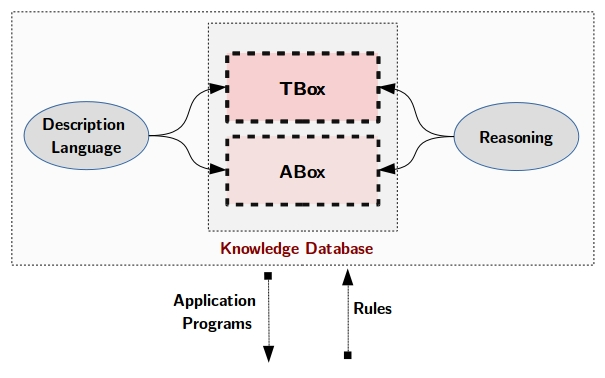
\includegraphics[scale=0.7]{figures/state_fig6}
			\caption{A knowledge Representation System Architecture of a knowledge
				representation system based on Description \citep{Baader2003}}
			\label{state_fig6}
		\end{figure}

		Description Language-based knowledge base $\mathcal{K}$(or an ontology) can be defined as 
		a pair $\mathcal{K} = (\mathcal{T}, \mathcal{A})$  where $\mathcal{T}$ (called the \emph{TBox}), 
		is a set of \textit{concept axioms} and \textit{role axioms}, and $\mathcal{A}$ (called the 
		\emph{ABox}), is a set of \textit{assertional axioms} (see figure \ref{state_fig6}).

		The \emph{concept axiom} has the form $C \sqsubseteq D$ where $C$ and $D$ are concept expressions.
		The \emph{role axiom} \revAnglais{has} the form $R \sqsubseteq S$ where $R$  and $S$ are role expressions. 
		Finally, the \emph{Assertional axioms} have the form $C(a)$ where $C$ is a concept and $a$ 
		is an individual name, or that have the form $R(a,b)$, where $R$ is a role and $a$ and $b$ 
		are individual names.

		In the Description Language, an interpretation $I$ is defined as follows: $I=\mathcal{I} 
		= \langle{}\triangle^{\mathcal{I}}= , \cdot^{\mathcal{I}}\rangle{}$ that consists of
		a non-empty set $\triangle^{\mathcal{I}}$ and an interpretation function $\cdot^{\mathcal{I}}$, 
		which maps from individuals, concepts and roles to elements of the domain, subsets of the domain 
		and binary relations on the domain, respectively.

		For a given interpretation $\mathcal{I} $, we can say that $\mathcal{I} $ satisfies a concept 
		axiom $C \sqsubseteq D$  (respectively $R \sqsubseteq S$) if $C^{\mathcal{I}} \subseteq 
		D^{\mathcal{I}} $ (respectively $R^{\mathcal{I}} \subseteq S^{\mathcal{I}}$). Moreover, 
		$\mathcal{I}$ satisfies a concept assertion $C(a)$ (respectively $R(a,b)$) if 
		$a^{\mathcal{I}} \in C^{\mathcal{I}}$ (respectively $(a^{\mathcal{I}},b^{\mathcal{I}}) 
		\in R^{\mathcal{I}}$).

		An interpretation $\mathcal{I}$ is called a model of an ontology $\mathcal{K}$ if and only 
		if it satisfies each axiom in $\mathcal{K}$. A concept name $C$ in an ontology $\mathcal{K}$, 
		is unsatisfiable if for each model $\mathcal{I}$ of $\mathcal{K}$, $C^{\mathcal{I}} = \varnothing$. 
		An ontology $\mathcal{K}$ is incoherent if there exists an unsatisfiable concept name in $\mathcal{K}$. 
		An ontology $\mathcal{K}$ is inconsistent if and only if it has no model.

		DL languages are identified with the concept constructors that they allow. For instance, the minimal 
		propositionally closed language allowing for the constructors $\sqcap$ ( conjunction), $\sqcup$ 
		(disjunction), $\neg$ (negation), $\forall$ (value restriction) and $\exists$ (existential restriction)
		is called $\mathcal{ALC}$. In \citep{Baader2003}, the author enumerates all the constructors used to 
		identify various Description Logic formalisms ($\mathcal{N}$, $\mathcal{Q}$, $\mathcal{O}$,
		$\mathcal{F}$, $\mathcal{U}$, \dots{}).

		Once a description of application domain using DL, the latter can make inference through 
		deducing implicit consequences from the explicitly represented knowledge. The subsumption is 
		the basis inference on concept descriptions: given two concept descriptions $C$ and $D$, 
		the subsumption problem $C \sqsubseteq D$ is the problem of checking whether the concept description 
		$D$ is more general \revAnglais{than} the concept description $C$. Then, the subsumption problem tries to determine whether 
		the first concept denotes in every interpretation a subset of the set denoted by the second one. $C$ 
		is subsumed by $D$, with respect to a \emph{TBox} $\mathcal{T}$, if in every model of $\mathcal{T}$, 
		$D$ is more general than $C$, i.e., the interpretation of $C$ is a subset of the interpretation of 
		$D$. This can be denoted as $C \sqsubseteq_{\mathcal{T}} D$.

		Description language based ontologies have been successfully used to achieve some interesting
		reasoning capabilities in the context of semantic multimedia analysis. In fact, such an ontology 
		formalism enables an intensive use of inference rules on the managed knowledge to perform advanced 
		multimedia semantic analysis, attaining thus a semantic interpretation that a human perception and 
		cognition can deliver. In order to achieve such an inference tasks, the description language \revAnglais{is} 
		based on a set of concepts and relationships between them. The lattes are called roles 
		(denoted with $\mathcal{R}$). Axioms are used to capture the conditions that need to be met 
		by consistent and coherent interpretations (the states of the domain). Therefore, the knowledge 
		management tasks within an ontology could be formalized as:

		\begin{itemize}
			\item \textbf{\textit{Deduction:}} is a task where the interpretation is an instantiation of 
			formal knowledge consistent with evidence about the real-world domain 
			\citep{Hartz2007,Hudelot2008,Dasiopoulou2009a}.
			
			\item \textbf{\textit{Abduction:}} is a task where the interpretation is an instantiation of 
			formal knowledge which allows to deduce the evidence \citep{Shanahan2005,Peraldi2007,Atif2014}.
		\end{itemize}
		The deduction and the abduction reasoning tasks were introduced as inference standards. 
		For the deduction reasoning, if $\sum$ is a logical theory and $\alpha$ a set of facts, 
		through deduction is verified whether $\varphi$ is logically entailed, that is whether $\sum, 
		\alpha \models \varphi$. For the abduction reasoning, given $\sum$ and $\varphi$, the abduction 
		consists in looking for an \emph{explanation} $\alpha$ so that the entailment $\sum, \alpha \models 
		\varphi$ is true.

		In \citep{Neumann2008,Moeller2008,Dasiopoulou2010,Bannour2014}, a comprehensive survey on 
		the use of formal (description language based) ontologies for multimedia semantic analysis
		is exposed. In the following section, we enumerate some of these works.

		



		\subsection{Related Work on Knowledge-Based Approaches for Multimedia Analysis}

		In the last fifteen years, ontologies have been emerged from an interesting conceptualization paradigm 
		to a very promising modeling technology for multimedia retrieval. Ontologies enable meaning driven 
		retrieval process through a machine-understandable form of a content description. 
		In the following, we enumerate some multimedia ontologies outlining main characteristics.

		The \emph{Harmony} ontology \citep{Hunter2001}, the \emph{aceMedia} ontology 
		\citep{ Petridis2004} and the	\emph{Rhizomik} \citep{Garcia2005} ontology are first initiatives 
		to attach formal semantic to MPEG-7.  These ontologies have been explored to support 
		semantic image /video analysis and annotation, addressing many content domains, including 
		pancreatic cell images (for \emph{Hamony}),  soccer video (for \emph{Rhizomik}), \dots.  
		More recent MPEG-7 based ontologies, like \emph{SmartWeb} \citep{Oberle2007}, \emph{DS-MIRF} 
		\citep{Tsinaraki2007}, \emph{COMM} \citep{Arndt2007} and \emph{Boemie} \citep{Dasiopoulou2009}, 
		focused on a fully translation/mapping of the complete MPEG-7 specification into \emph{OWL}. 
		
		These ontologies were mostly used in analyzing and annotating sport oriented multimedia contents.
		In their majority, enumerated ontologies have been constructed manually, and their knowledge structures 
		are rather focused on low-level and high-level features (as classes), and their spatial-temporal 
		relationships for particular content domains. Thus, these approaches are limited to provide a 
		formalism that \revAnglais{allows} to use ontologies as repositories for storing knowledge. So, there is no
		correspondence between the expressive power provided by the adopted representation language, and 
		the constructed ontology definitions. Hence, the ontologies were not fully exploited for multimedia 
		retrieval. The key issue in enhancing multimedia retrieval is to focus to inherent semantics in addition 
		to extracted ones through exploring reasoning and deduction capabilities of ontologies. Indeed, and 
		contrary to the aforementioned ontologies, recent ontologies are addressing issues related to actual 
		research works handling semantic contexts and concept co-occurrence.

		Indeed, in \citep{Mylonas2009}, the authors proposed an ontology based approach to improve concept 
		detection through visual thesaurus and semantic contexts. The authors \revAnglais{introduce} thus the use 
		of semantic contexts in order to refine the confidence values for regions before taking decision.
		The latter deals with a proposed ontology that specifies fuzzy semantic relations among 
		concepts/contexts \emph{Location}, \emph{Property}, \emph{Part}, \emph{Similar}, \dots{}.

		In \citep{Simou2008}, the authors proposed a knowledge based framework for enhancing an initial 
		set of over-segmented regions. Spatial relations and neighborhood information are managed within
		an ontology. The latter is defined by $\mathcal{SHIN}$ description language formalism. 
		The authors proposed also a deduction engine called \textsc{Fire} in order to extract additional
		implicit knowledge.

		In \citep{Hudelot2010}, the authors proposed an ontology for spatial relations in order to 
		facilitate image interpretation. Such relations were considered as crucial for the semantic 
		concept detection task. The proposed ontology was defined by the $\mathcal{ALC(D)}$ description
		language formalism.

		In \citep{Bannour2014}, the authors proposed a framework for building and using structured 
		knowledge models for visual content analysis and annotation. The authors proposed thus an 
		ontology to build explicit and structured knowledge models dedicated to image annotation.
		The defined ontology used the $\mathcal{SROIQ(D)}$ description language formalism.
		The built ontology consists in conceptual, contextual and spatial knowledge about an image 
		(including relationships like \emph{isAnnotatedBy}, \emph{hasAppearedLeftOf}, 
		\emph{hasAppearedCloseTo}, \dots{}). The authors proposed also reasoning framework in 
		order to check about the consistency of the annotation efficiency.

		Another research works focused on improving the indexing efficiency through the use of
		the ontologies capabilities.  Indeed, in \citep{Leite2008,Cheng2012,Mukesh2013}, 
		the authors proposed an ontology based framework in order to enhance a semantic interpretation. 
		\revAnglais{These} works mainly focused on defining how  to manage knowledge in an ontology
		(concept and relationships). Also, other retrieval aspects were \revAnglais{dealt:} in 
		\citep{Rodriguez-Garcia2012}, the authors detailed how to evolve the ontology
		content using the \textsc{DBpedia} as an external data source. Also, in \citep{Mustafa2008}, 
		the authors  refined the semantic level by analyzing contexts and concepts interrelationships
		in a particular context. 
		
		In \citep{Reshma2014}, an ontology was generated and used both: (1) in training 
		phase to select images that should be used for optimizing classifiers, and (2)
		in testing phase for deducing new annotations through concept inter-relationships. 

		\subsection{Discussion}

		Recent research works are focusing on using ontologies for multimedia retrieval in order to allow
		semantic interpretation and reasoning over extracted descriptions. However, much remains to 
		be done in order to achieve less human aid ontology modeling approaches.

		Firstly, almost all existing approaches for modeling ontologies still relying on manual 
		knowledge population (knowledge defined by experts) and there is no explicit method 
		proposed for an automated ontology population. Such manual approaches are always costly, 
		not always relevant and incomplete.

		Secondly, using various relationships between concept/context has led to diversify the 
		semantic capabilities of an ontology (as proved by aforementioned approaches), 
		but it reduces their capacities to cover more multimedia content domains. Within
		an ontology structures, many semantic relationships between concepts were defined:
		 \emph{is-a} 	and \emph{has-part} in \textsc{WordNet} \citep{Fellbaum2010}, 
		\emph{is-a} in \textsc{LsCom} \citep{lscom2006}, \emph{IsPartOf}, \emph{Location}, 
		\emph{Property}, \emph{Part}, \emph{Similar}, 	\dots in \citep{Mylonas2008,Mylonas2009}. 
		We suppose that the generic aspect of an ontology strongly depends \revAnglais{on} its ability to model 
		any semantic relationship between concepts/contexts. 

		Thirdly, the scalability should be considered in modeling ontologies, particularly, 
		for the ontology structure effectiveness and reasoning computational cost. While in 
		\citep{Simou2008,Hudelot2010,Paliouras2011,Bannour2014}, the ontology structure is 
		defined by a highly expressive language, a \revAnglais{simpler} structure and less expressive 
		language is used in  \citep{lscom2006,Vallet2007,Mylonas2008,Mylonas2009,Fellbaum2010}.
		Expressive language level is tweaked by paying attention to the huge amount of 
		computational tasks needed for video interpretation. In fact, a simple ontology structure 
		could be a good accommodation between a video analysis speed and performance.

		Finally, the context of a content could provide an important cue for enhancing a semantic
		interpretation \citep{Fauzi2014}.  Yet, the definition of a context remains unclear and there 
		is no computational method to define it. Contexts are defined manually in all works 	
		listed above. We consider that a computational definition of a context is a crucial 
		step for an automated ontology construction.

		The ontology \revAnglais{used} in the indexing process should also address issues related to 
		actual research works dealing with the indexing process. Indeed, the use of 
		\emph{context} and handling the uncertain aspect of a semantic interpretation 
		of video contents are also substantial. In the next section, we discuss handling 
		uncertain information and knowledge in multimedia content analysis.

	\section{Uncertain Knowledge Management}

		In literature, there is several valuations about the selection between a fuzzy 
		or probabilistic approaches regarding handling uncertain knowledge. Furthermore, 
		Knowledge managing and ontology engineering attracted many research communities, 
		but in multimedia retrieval one, some specific considerations have to be taken into account.

		\subsection{How to manage the uncertainty}

		Knowledge discovery is related to the analysis of large contents in the purpose of 
		extracting valuable, meaningful, unknown and unexpected relationships. Real world data is 
		characterized by the vagueness and the uncertainty of its content.
	
		In multimedia retrieval, discovering knowledge from annotated multimedia contents are
		considered as an important task in order to handle semantics efficiently. 
		Yet, there are many cases in which annotated contents display uncertain situations. 
		In literature, two approaches attracted the attention of many researchers in order 
		to handle uncertain \revAnglais{knowledge:} the probability theory and the fuzzy logic.

		As discussed above, these annotated video datasets comprise naturally
		many uncertain situations. So, we adopted a fuzzy logic based approach \citep{zadeh3,zadeh2,zadeh1}
		to handle such situations because we believe that such approach fits better than probabilistic 
		ones for managing uncertain knowledge, and it was widely adopted by many works that 
		deal with uncertainty in multimedia retrieval
		\citep{Bloch2005,Hudelot2008,Simou2008,Dasiopoulou2009,Bannour2014}.

		Indeed, the probabilistic approaches are based on estimating probability that 
		a data belongs to a class. On the other hand, fuzzy approaches attribute for 
		a given data different degrees of membership to classes. Thus, the fuzzy logic 
		handles a type deterministic uncertainty describing the data class ambiguity. 
		And unlike the probabilistic approaches which answer to the question if a data 
		belongs or not to a class, the fuzzy ones compute the degrees to which a data 
		belongs to a set of classes. Then, the fuzzy logic considers that a data could 
		belong to a set of classes at the same time with different membership degrees.  
	
		When analyzing a multimedia content, we intend generally to annotate that content by 
		a set of semantic concepts. For each one, a degree of membership is computed in 
		order to describe if that semantic concept figures or not in the content. 
		This degree is ranging from $0$ to $1$, and there are some situations where 
		it is hard to say if the concept really exists ($1$) or not ($0$). Furthermore, 
		this degree is generally confounded with the probability (between $0$ and $1$) 
		that a semantic concept exists in a content. So, even the probability and 
		the fuzzy membership are ranging from $0$ to $1$, they are fundamentally
		different.

		To conclude, and in literature, there are many discussions about these 
		two approaches and their efficient capabilities to handle and support uncertainty. 
		In fact, many arguments are defended by the knowledge extraction community about 
		the effectiveness of fuzzy approaches and probabilistic ones 
		\citep{Gaines1978,Bosko1990,Sanjaa2007,Zadeh2014,Zadeh2015}. In our work, we focused on the use of a
		fuzzy approach not for proving that such an approach is better than the probabilistic ones, 
		but because we believe that fuzziness 
		is more suitable for our case.

		\subsection{Fuzzy DLs}
		Despite the expressiveness of DLs, they lack the ability to handle vague and uncertain semantics 
		which is a real requirement in multimedia content indexing \citep{Simou2008}.  In fact, as stressed 
		in this dissertation, multimedia retrieval faces the problem of handling uncertain information 
		about multimedia contents.

		In order to cope with the uncertainty issue in multimedia indexing,  \emph{Fuzzy-DL} 
		\citep{Stracci1998,Straccia2006,Stoilos2007,Ma2013} is considered as an interesting 
		formalism for representing a multimedia ontology. In fact, the fuzzy Description Logics
		is considered as a very interesting logical formalism as it can be used in numerous domains
		like multimedia and information retrieval \citep{Meghini2001} to provide ranking degrees and 
		to cope with vague concepts like \emph{“near”}, \emph{“far”} and many more.

		Fuzzy logic deals with vagueness and imprecision using fuzzy predicates. Therefore,
		the fuzzy logic offers a considerable foundation for description language generalization 
		in order to deal with such vague concepts. Thus, fuzzy DL allows expression of the form 
		$(\langle{}C(a) \geq n\rangle$ where $n \in [0..1]$, ie $(\langle{}Far(distance) \geq 0.7\rangle$, 
		with intended meaning “the membership degree of individual $a$ being an instance of concept $C$ 
		is at least $n$”. 

		In the two last decades, many fuzzy description logic formalisms were discussed and proposed. 
		The fuzzy aspect integration into DL does not concern only adding role hierarchies and number 
		restrictions, but also the decidability proof and decision procedures for the knowledge 
		base satisfiability and consistency. 

		For instance, in \citep{Stracci1998}, the authors proposed the fuzzy integration within 
		the DL $\mathcal{ALC}$ formalism with taking an attention on a nice trade-off between 
		computational complexity and expressive power of DLs.

		In \citep{Stoilos2005a,Stoilos2007}, the fuzzy $\mathcal{ALC}$ is extended to the fuzzy 
		$\mathcal{SHIN}$ with transitive role axioms ($\mathcal{S}$), inverse roles  ($\mathcal{I}$),
		role hierarchies ($\mathcal{H}$) and number restrictions ($\mathcal{N}$). The main contributions 
		in such a work are a detailed reasoning algorithms, and the decidability proof of the fuzzy DL 
		fuzzy-$\mathcal{SHIN}$. In \citep{Simou2007,Simou2008}, fuzzy-$\mathcal{SHIN}$ was used as a 
		formalism to construct and manage an ontology for a multimedia content analysis process.

		In \citep{Straccia2006}, the authors proposed a fuzzy extension of the OWL Description language
		formalism $\mathcal{SHOIN}$. The latter was also extended to in \citep{Stoilos2006} to 
		fuzzy $\mathcal{SHOIQ}$ investigating several properties of the semantics of transitivity, 
		qualified cardinality restrictions and reasoning capabilities.

		In \citep{Bannour2014}, fuzzy-$\mathcal{SROIQ}$ was proposed in the aim to provide both a 
		set of constructors allowing the construction of new concepts and roles. This formalism
		includes $\mathcal{ALC}$ standard constructors (i.e. negation, conjunction , disjunction,
		full existential quantification, and value restriction) extended with transitive roles 
		($\mathcal{S}$), complex role axioms ($\mathcal{R}$), nominals ($\mathcal{O}$), inverse 
		roles ($\mathcal{I}$), and qualified number restrictions ($\mathcal{Q}$). The proposed 
		fuzzy DL formalism is used to manage an ontology that supports an image annotation framework.

		To sum up, many extensions are raising more and more on the crisp DL in order to enable 
		handling uncertain and vague knowledge through the use of fuzzy logic theory. Thus, 
		a great variety of fuzzy DLs can be found in the literature \citep{Garci2010,Cerami2013}. 
		Nevertheless, it has been shown that several fuzzy Dl formalisms face the undecidable 
		reasoning issue \citep{Baader2011}. In fact, the fuzzy extensions of DL {do} not have 
		the finite model property, then the proposed reasoning algorithms are neither correct nor 
		complete: the knowledge base satisfiability is then an undecidable problem \citep{Cerami2013}. 
		Despite many efforts to proof the decidability of fuzzy DL, multimedia spatial-temporal 
		reasoning based on description logic is well known as undecidable. This is due to specific 
		nature of spatial temporal information to be handled. In fact, this information is 
		cyclic and transitive, and within this particular situation, the fuzzy DL formalisms are undecidable.


		\subsection{Discussion}

		As discussed in chapter \ref{intro}, we intend to go deeper in the exploitation of ontology
		semantic capabilities in order to improve the video analysis process, and particularly, 
		the indexing one. Our objective is twofold. Firstly, we aim to define an approach to extract, 
		by an automatic manner, valuable knowledge from a video annotated dataset. Secondly, 
		we show how we construct an ontology that includes conceptual and contextual knowledge 
		and populated by the extracted knowledge. 

		We focus on solving the main issues related to managing knowledge in multimedia \revAnglais{retrieval:} 
		uncertainty and the large amount of data to be treated. As aforementioned, a fuzzy approach 
		is adopted to handle uncertainty. On the other hand, we \revAnglais{intend} to propose an approach that 
		could enable a machine to discover new knowledge from large-scale multimedia datasets, and 
		to reason about a multimedia semantic interpretation in order to enhance it.  However, 
		analyzing large-scale video datasets to explore and reason with their contents is a critical
		task particularly when using \emph{Description Logics} (DL) as a formal description of ontology 
		content and reasoning \citep{Stoilos2005,Dasiopoulou2010,Bannour2014}. Then, in our dissertation, 
		we aim to define an alleviated ontology structure using \emph{fuzzy-DL}, and a tweaked reasoning 
		engine in order to enhance video content descriptions with an acceptable computing cost. 



	\section{Multimedia Retrieval Scalability}

		\subsection{The scalability issue}

		Nowadays, multimedia analysis tools and applications require a real-time processing, in particular 
		when embedded within interactive environments such as smart-phones and home entertainment systems. 
		A such real time processing needs fast and low-latency approaches for multimedia analysis. 
		With such an intensive computing demands, the multimedia retrieval is faced with the problem: 
		how do the multimedia analysis efficiently process the growing amount of data and how to define 
		scalable approaches that could meet user requirement?

		In order to enable multimedia retrieval scalability to the huge amount of multimedia data, 
		the literature proposed \revKarray{three} different research directions: The first direction deals 
		with the use of cloud and distributed programming frameworks such as \emph{Multi-Threaded Processing} 
		\citep{Amit2006},  \emph{Hadoop} \citep{White2012,Landset2015}, \emph{MapReduce} 
		\citep{Dean2008,Dean2010} \revKarray{and \emph{Apache Spark} \citep{Meng2016,Zaharia2016}}.
		\revKarray{The second direction deals with deep neural networks based methods and 
		techniques \citep{Long2016} in order to address the scalability.}
		The third direction deals with semantic hierarchies 
		\citep{Deng2010,Zhou2014,Ordonez2015} in order to reduce the complexity of managing 
		large scale data through the use of some heuristics.
		
		In what follows, we enumerate some
		research \revAnglais{works} that aimed to solve the scalability issue through 
		these three different directions.

		\subsection{Cloud/distributed-Based Approaches}
		
		\revKarray{Cloud and distributed based approaches provide powerful technology 
		and techniques to perform massive-scale and complex computing \citep{Furht2010,Zhu2010}.
		Due to the time demanding multimedia analysis task that requires a large computational framework, 
		the multimedia community addressed cloud and distributed approaches \citep{Zhu2011}.}
		
		In \citep{Mohamed2012}, the authors proposed an adapted structure of \emph{MapReduce}
		programming model for a scalable multimedia indexing. With an experiment contacted on 
		\emph{XML} text and images from \textsc{ImageNet}, they achieved a good speed compared to 
		a sequential implementation.
	
		In \citep{Guhmundsson2012}, the authors described a study where the \emph{Hadoop} 
		parallel and distributed run-time environment is used to speed up the 
		construction of a large high-dimensional index
		for multimedia contents. They achieved then a speed-up of about $400 \%$ 
		compared to a classical index construction. 
		
		In \citep{Mourao2015}, the authors proposed a \emph{Hadoop} distributed search engine framework.
		They considered that such a framework is flexible enough to support and handle several millions
		of multimedia contents.

		In \citep{Chen2008,Luo2008,Lopresti2012,Oh2015,Osipyan2015}, the authors exposed different 
		research works on the use of \emph{GPU} (Graphical Processing Unit) in order to parallel
		the heavy computing process for different multimedia analysis tasks: face detection, 
		features extraction and classification, \dots{}.

		\revKarray{In \citep{Kumar2015}, the authors focused on modeling a high performance video data processing 
		technique. The latter uses a \textsc{GPU} based parallel implementation of object detection algorithm.}

		\subsection{Deep Learning-Based Approaches}
		
		\revKarray{Deep learning \citep{Hinton2006,Hinton2006a,Bengio2009} can be defined as a set 
		of machine learning algorithms that can learn the data representation and feature extraction
		with many layers of non-linear transformations. A typical deep learning architecture 
		consists of artificial neural network with many layers of non-linear processing 
		units \citep{Haykin2004,Jaeger2016}.}
		
		\revKarray{Actually, we observe that Deep learning is a thriving field with many practical 
		applications and research topics, including semantic object detection
		\citep{Hinton2006a,Bengio2007,Ciregan2012,Krizhevsky2012} and information retrieval 
		\citep{Salakhutdinov2009,Hinton2011}.}
		
		\revKarray{In conjunction with significant gain in machine performances (particularly with 
		\textsc{GPUs} based acceleration), the massive amount of labeled data available for supervised 
		training allowed the deep neural networks to significantly improve the machine learning abilities 
		for a variety of applications \citep{Long2016}. The amount of multimedia data has grown to an extend
		that classical multimedia processing and analysis techniques are unable handle data effectively 
		\citep{Jiang2015}. In fact, some deep neural networks based methods and techniques were proposed 
		in order to address the scalability issue and to handle large amount of multimedia data. 
		\citep{Wu2015,Druzhkov2016} display a comprehensive survey on deep learning methods and software
		tools for video segmentation, image classification, object detection, audio analysis, ....}

		\revKarray{In recent literature, a growing number of research work are being the effectiveness of
		deep neural networks based methods in handling the scalability issue, in particular 
		\textit{Deep Convolutional Neural Networks} (CNN).}
		
		\revKarray{Indeed, in \citep{Jiang2015} used CNN for large scale image feature extraction and classification. 
		In \citep{Sainath2015}, CNN are used for large scale speech analysis. In \citep{Girshick2014}, CNN are also efficiently used for image 
		region detection, feature extraction, object detection and semantic segmentation.
		In \citep{Tong2015}, a CNN based framework for large scale video shot boundary detection
		and semantic  annotation is detailed.}

		\subsection{Semantic hierarchies-Based Approaches}

		Despite the significant progress shown by the above enumerated works to achieve a 
		scalable multimedia analysis frameworks and approaches, 
		\revKarray{and in particular deep neural networks based ones,} 
		some other works attempt to 
		use the reasoning power of the ontologies for the semantic multimedia content interpretation 
		and analysis. In fact, a formal model of a given knowledge can be used  in order to help
		and guide the semantic multimedia analysis, and then to alleviate its computational cost.

		Semantic hierarchies \citep{Simou2005,Fan2008,Deng2009} were proposed to construct 
		\revAnglais{semantic relationships} between semantic concepts. Such a hierarchy could be used then
		to alleviate the multimedia analysis process, and then to be able to handle large-scale multimedia contents.

		In \citep{Dasiopoulou2008,Dasiopoulou2009a}, the authors proposed an approach for 
		reasoning on the output of a statistical classifiers. In fact, the extracted
		descriptions about a content are used within a reasoning process in order to look for 
		extra semantic concepts that were not detected by the statistical classifiers. 
		Likewise, in \citep{Hudelot2010,Bannour2014}, the authors proposed to use a built 
		knowledge model in a framework for reasoning over the outputs of machine learning algorithms. 

		\subsection{Discussion}

		To sum up, we think that the literature exposed many research works to enable the multimedia 
		indexing capabilities for handling large-scale data. In this dissertation, we are more oriented
		towards semantic hierarchies based approaches rather than distributed and parallel ones. 
		In fact, we think that giving a built knowledge database about semantic concepts/contexts 
		relationships, the semantic hierarchy could be used to enhance the semantic analysis efficiency. 
		
		Furthermore, we observe that semantic hierarchy based approaches focused on late guiding 
		the semantic concept detection. In fact, these approaches handle the output of semantic 
		concept detectors, and not the detectors themselves. Thus, we think that the valuable 
		knowledge stored within an ontology could contribute at the enhancement of 
		multimedia analysis efficiency through guiding the construction of the concept detectors. 
		
		The chapter \ref{c3} exposes our contribution for a scalable multimedia content indexing 
		through a framework that constructs semantic concept detectors based on knowledge reasoning.


	\section{Evaluation of Literature Review}

		Actually, there is yet standard approaches which can be used for indexing a
		video content. The latter can be indexed based on either the low-level (perceptual) 
		features or high-level (semantic) annotation. As already discussed in the previous
		chapters, such approaches fail to alleviate the semantic gap issue. This dissertation 
		aims to show the benefits of integrating
		fuzzy knowledge based approaches in the video indexing process. Nevertheless, such new
		approaches must be standardized, generic and robust enough to be applied for different user
		and application requirements.

		By drawing on the semantic assets provided by the two proposals 
		(namely the concepts co-existence and contexts), the multimedia 
		community investigated the knowledge engineering for multimedia retrieval. 
		As a  knowledge database, the ontologies are considered as powerful 
		tool to design and handle concepts/contexts and their interrelationships. 
		Ontology-based multimedia retrieval approaches focus on defining a knowledge 
		conceptualization and a reasoning process in order to analyze and improve 
		semantic interpretation of a multimedia content. Ontology-based approaches 
		for semantic multimedia retrieval displayed promising results \citep{Kannan2012}. 
		However, new issues appeared and further researches on ontology engineering for 
		multimedia analysis have to be more addressed.

		Based on the literature review, the tables \ref{review1}, \ref{review2} and \ref{review3} expose 
		some main characteristics of the three video indexing approaches.
		\begin{table}
			\footnotesize
			\centering
			\caption{Literature Review on Knowledge-based Multimedia Analysis}
			\begin{tabular}{p{4.7cm}  p{4.7cm}p{4.7cm}}
 				%\hline	
				\textbf{\sffamily Approaches} & \textbf{\sffamily Advantages} & \textbf{\sffamily Limits} \\  \hline
				\begin{flushleft} {\textbf{Earlier approaches: Mapping low-level features to an ontology}} \end{flushleft}
				& \begin{flushleft} Provided a rich set of standardized tools that generate 
					and understand multimedia content.\end{flushleft}
				& \begin{flushleft} Focused only on mapping low-level features to an \revAnglais{ontology} 
					without availing its reasoning capabilities.\end{flushleft} \\
				%\hline
				\begin{flushleft} {\textbf{Lite ontologies for semantic analysis}} \end{flushleft}
				&  \begin{flushleft} - Model knowledge as classification, categorization and 
					taxonomies for many application domains. \par
				   - Model semantic concept inter-relationships and semantic contexts 
					in order to provide a more semantic level for the interpretation of
					a multimedia content.\end{flushleft}
				&  \begin{flushleft} Handle explicit knowledge without exploring implicit one: the reasoning 
					capabilities of an ontology are not availed.\end{flushleft}\\
				%\hline 
				\begin{flushleft} {\textbf{Formal ontologies for semantic analysis }} \end{flushleft}
				& \begin{flushleft}- Provide a powerful expressiveness and formal knowledge representation. \par
				  - Supply many reasoning capabilities to infer implicit knowledge. \par
				  - Contribute to enhance multimedia indexing through inferring inherent 
					semantics in addition to extracted ones through exploring reasoning 
					and deduction capabilities of ontologies.\end{flushleft}
				& \begin{flushleft}
					- The proposed approaches rely on manual knowledge population: 
					a costly task and not always relevant and complete. Semantic 
					concepts inter-relationships and contexts are defined manually.\par
					- Many semantic concepts/contexts inter-relationships are defined 
					depending on the application domain to handle. So, no generic 
					knowledge structure \revAnglais{was} proposed.\par
					- No real discussion about the scalability of the proposed formalisms
					and their capabilities to deal with real large-scale data. \par
					- No generic multimedia analysis oriented framework proposed to manage 
					the complete knowledge work-flow within an ontology: knowledge abduction, 
					population, reasoning and evolving.
				\end{flushleft}\\
				\hline
			\end{tabular}
			\label{review1}
		\end{table}

		\begin{table}
			\footnotesize
			\centering
			\caption{Literature Review on Fuzzy-DL Formalisms to Handle Uncertain Knowledge}
			\begin{tabular}{p{4.7cm}  p{4.7cm}p{4.7cm}}
 				%\hline	
				\textbf{\sffamily Approaches} & \textbf{\sffamily Advantages} & \textbf{\sffamily Limits} \\  \hline
				\begin{flushleft} {\textbf{Fuzzy-DL formalisms for Multimedia ontologies}} \end{flushleft}
				& \begin{flushleft}
					- Fuzzy logic deals with vagueness and imprecision using fuzzy predicates. 
					Therefore, the fuzzy logic offers a considerable foundation 
					for description language generalization in order to deal with such vague concepts. \par
					- A variety of fuzzy-DL formalisms \revAnglais{is} proposed, and many reasoning engines 
					were developed.\par
					- Widely emerged in recent knowledge-based multimedia semantic analysis. 
					Thus Many fuzzy-DL formalisms are being used to construct and 
					manage an ontology for a multimedia content analysis process.
				 \end{flushleft}
				& \begin{flushleft} 
					- Fuzzy-DL faces the undecidable reasoning issue. 
					In fact, semantic concepts/contexts inter-relationships are 
					often cyclic, transitive which make the reasoning task 
					undecidable.\par
					 - No real discussion about the scalability of the proposed formalisms
					and their capabilities to deal with real large-scale data. \par
				  \end{flushleft} \\
				\hline
			\end{tabular}
			\label{review2}
		\end{table}
 
		\begin{table}[hb!]
			\footnotesize
			\centering
			\caption{Literature Review on Scalable Multimedia Indexing approaches}
			\begin{tabular}{p{4.7cm}  p{4.7cm}p{4.7cm}}
 				%\hline	
				\textbf{\sffamily Approaches} & \textbf{\sffamily advantages} & \textbf{\sffamily Limits} \\  \hline
				\begin{flushleft} {\textbf{Parallel based approaches }} \end{flushleft}
				& \begin{flushleft}
					- A significant and spectacular speed-up for multimedia analysis frameworks 
					and approaches through  parallelizing the computing task. \par
					- \emph{MaprReduce}, \emph{Hadoop} and in particular \textsc{Cuda} 
					are getting more and more \revAnglais{engendered} to accelerate heavy computing 
					works for many research fields. 
				 \end{flushleft}
				& \begin{flushleft} 
					The parallelization is defined manually by the developers and 
					generally considered as a complex task.
				  \end{flushleft} \\

				\begin{flushleft} {\textbf{\revAnglais{Knowledge} based approaches}} \end{flushleft}
				& \begin{flushleft}
					- The  reasoning power of the ontologies are potential formalism that 
					could help and guide the semantic multimedia analysis, and then  
					alleviate its computational cost. \par
					- Semantic concepts/contexts inter-relationships could be potential information
					that could generate some heuristics for the detection of large set of semantic concepts
					within a multimedia content.
				 \end{flushleft}
				& \begin{flushleft} 
					The semantic concepts hierarchies are used to enhance the outputs
					of semantic concept detectors. But few works are interested in 
					integrating of such hierarchies within the construction 
					process of these detectors.
				  \end{flushleft} \\
				\hline
			\end{tabular}
			\label{review3}
		\end{table}

		
		In this dissertation, we are focusing on the semantic video indexing through exploring ontologies
		structures and semantic capabilities. The latter are used to improve the multimedia indexing process,
		and to build a scalable indexing tool. Specifically, our concerns in this dissertation are as follows: 
		
		Firstly, we look for a generic knowledge-based framework that handle multi-modal interpretations
		in order to deduce a more complete semantic representation for a multimedia content through 
		ontologies capabilities (basically abduction and deduction). 

		Secondly, we focus more on the ontology management side, and we define a complete automatic 
		knowledge manager: from extracting valuable knowledge, defining the ontology structure by 
		taking into consideration semantic context and concept co-occurrence, and the deduction 
		process that generates an enhanced interpretation over ones delivered by classical
		semantic concept detectors, to the knowledge evolving. The proposed ontology \revAnglais{profits}  
		from the expressiveness and reasoning power of fuzzy-DL formalisms with paying 
		attention to the scalability issue.
	
		Thirdly, we explore more the ontology \revAnglais{while} focusing on exploring their content to build 
		scalable semantic concept detectors. Subsequently, we aim to use knowledge model in order 
		to produce a semantically consistent and scalable multimedia indexing process.


	\section{Conclusion}
		In the present chapter, we exposed a comprehensive overview on the recent work for 
		multimedia retrieval, and particularly the multimedia indexing. Our aim was not to provide 
		a complete survey of the state of the art approaches, but to show the importance of knowledge 
		based approaches for multimedia indexing problems and to shed light \revAnglais{on} the benefits of each of them. 
		In fact, exploring ontologies seems to be essential to improve the multimedia indexing, 
		and then to narrow the semantic gap. 

		The next chapter will present our first contribution that is revealed by the defintion
		of a generic framework for a multimedia semantic indexing.




	\part{Fuzzy Ontology Based Framework for Video Indexing}
			\chapter{Multimodal Fuzzy Fusion Framework for Semantic Video Indexing Improvement}
\label{c1}

		%The availability of large-scale video annotated datasets constitutes a crucial requirement 
		%for promoting knowledge discovery. Many annotation tools were provided \citep{Dasiopoulou2011}
		%(such as \emph{VIA}, \emph{VideoAnnEx}, \emph{Ontolog}, \emph{Advene}, \emph{Elan}, \emph{Anvil},
		% \dots). These tools investigate spatial-temporal information in a video content. However,
		%no standardized large-scale annotated video dataset was officially proposed. Particularly, 
		%\textsc{TrecVid} \cite{Over2013} proposed a standardized annotated video dataset used for
		%measuring video retrieval and indexing performances. 

	

	In this chapter, we detail and discuss the first contribution $C_{1}$. In fact, we propose a general 
	multimodal fuzzy approach to enhance video semantic indexing accuracy. The latter approach was developed 
	incrementally through some consecutive research works. For that, and in the section \ref{c1_1}, 
	we first introduce our preliminary reflections for a knowledge based framework to index video content 
	efficiently. Then, in section \ref{c1_2}, and based on what was obtained through an experimental study, 
	we present a framework improvement, in particular, handling fuzzy knowledge and corresponding reasoning 
	ability. Finally, in section \ref{c1_3}, we present our proposed video annotation tool in order to generate 
	valuable data source about video content. First of all, section \ref{c1_0} displays first \revAnglais{afterthought}
	for a knowledge based video indexing framework.

	\section{Context and Motivation}
	\label{c1_0}

	Multi-modal fusion has gained much attention by the multimedia community \citep{Atrey2010}. 
	In fact, a video indexing task involves processing of multi-modal data in order to obtain valuable 
	insights about the content. Such a task could use sensory data (such as audio and visual analysis) 
	as well as \revAnglais{non-sensory} data (such as meta-data). Thus, the fusion of multiple modalities can provide 
	complementary information and increase, then, the accuracy of the indexing process.
	
	In \citep{Lucien1999}, the data fusion is defined as follows:
		\begin{definition}
			''a formal framework in
 		which are expressed means and tools for the alliance of
 		data originating from different sources. It aims at obtaining
 		information of greater quality''.
	\end{definition}

	A discussed in \citep{Waltz1990,Esteban2005,Blasch2006,Guerrero2009}, a fusion process 
	consists of five levels: The \emph{level 0} (named  \emph{pre-processing}) and \emph{level 1}
	(named \emph{object refinement}) cover respectively signal processing and data alignment. 
	The \emph{level 2} (named \emph{situation refinement}) attempts to \revAnglais{construct} a complete picture 
	from incomplete information provided by the lower levels (\emph{level 0} and \emph{level 1}).
	The \emph{level 3} (named \emph{threat refinement}) interprets the results from \emph{level 2} 
	in terms of the possible opportunities for operation. A \emph{process refinement},
	referred to \emph{level 4}, loops around these earlier levels to monitor performance 
 	and optimize the fusion process. Earlier data fusion applications were initially used for
	military reasons. But currently, data fusion model is extended for several other 
	areas \citep{LigginsII2008}.

	By drawing inspiration from this fusion model, we propose a fusion framework to fuse 
	multi-modal video content extracted semantics (concepts). Thus, we adopt the
	\textsc{Jdl/Dfs} data fusion model \citep{Waltz1990}.

	After an experimental study carried out within \textsc{TrecVid2010} evaluation campaign,
	we concluded that the multi-modal fusion process is important, but a big challenge occurred on 
	how to efficiently manage and explore fuzzy knowledge for better semantic indexing enhancement. 
	From this observation, we decided to tackle in depth the knowledge management raised issue. 
	Thus, we proposed a preliminary fuzzy ontology based framework to explore knowledge reasoning 
	capabilities in video indexing. A light ontology structure was proposed, as well as \revAnglais{an} abduction 
	engine to extract fuzzy knowledge from valuable data sources, and a deduction engine able to 
	leverage from the extracted knowledge in order to generate newer knowledge filling out a semantic
	interpretation about a video content.

	Yet again, the experimental study showed that the use of contextual ontologies has improved 
	the indexing process performances, however good, a simple set of manually defined contexts 
	were used. Aiming to go further in the use of contextual information, we proposed afterwards 
	a fuzzy video collaborative annotation tool that helps to detect potential semantic concept 
	inter-relationships. The latter are important to define semantic contexts.
		
	In the following section, we display in details main works that have been conducted 
	in order to \revAnglais{realize} our first contribution $C_{1}$.
	
	\section{A Multimodal Fuzzy Fusion Framework}
	\label{c1_1}

	
	In this section, we will introduce our fusion system and
	describe the multi-modal fuzzy fusion process.

	The proposed fusion architecture, based on the JDL/DFS model, is shown in figure \ref{fig:contrib1::fig1}. 
	After extracting unimodal semantic interpretation (level 0), the level 1 
	is called to search and eliminate conflicting situations. Then, level 2 
	is applied on level 1 results aiming at finding further concepts based 
	on abduction and deduction engines. These engines analyses relationships
	between concepts. The level 4 is used to control the whole fusion process. 
	Below is the description of the different integrated levels and the proposed fusion architecture.
	
	\begin{figure}[ht!]	
		\centering
		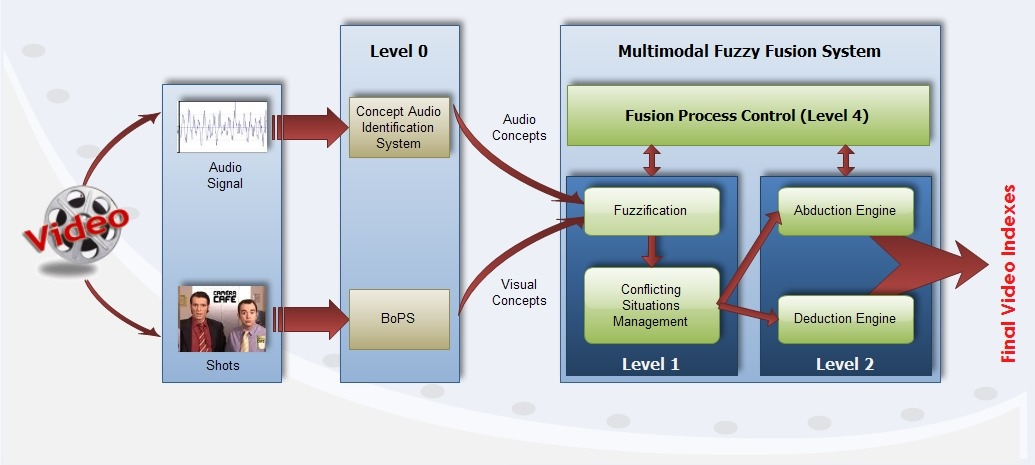
\includegraphics[width=\textwidth]{graphics/contrib1::fig1}
		\caption{Overview of the proposed Multimodal Fuzzy Fusion System}
		\label{fig:contrib1::fig1}
	\end{figure}

	\subsection{Object refinement (level 1)}
		The \emph{level 1} deals with mixed unimodal semantic interpretations. The latters are structured through 
		this data \revAnglais{format:} every concept has a list of indexed video content sorted by their descending 
		pertinent ranks. These ranks are fuzzified then analyzed.
		
		\begin{description}
			\item[Concept ranks fuzzification]
			The purpose of this step is to calculate the fuzzy membership
			degree of a concept to a video content. 
			This is given by a normalization function (see equation \ref{equation1}).

			Let $r$ be the rank of a concept for a video content, and $R$ is the highest 
			rank of the same concept for all video contents. We seek for a transformed rank called $r_{N}$ as follows:
			\begin{equation}
				\label{equation1}
				r_{N} = \left( \frac{(\epsilon -1)}{(R-1)} * (R-r) \right) +1 
			\end{equation}
			Where $\epsilon$ is a \revAnglais{positive} integer.

			\item[Conflicting situations handling]
		Sometimes, certain conflicting situations can be found in aggregated semantic interpretations.
		Since we are using fuzzy logic, two contradictory semantic interpretations can coexist for the 
		same video content. This situation is  permitted until the equation \ref{equation2} is verified.
		
		Let $c_{1}$ and $c_{2}$ be two contradictory concepts. And Let $\mu(c_{1})$ and $\mu(c_{2})$
		be respectively the relevance degree of the first and the second concepts. 

		\begin{equation}
			\label{equation2}
				\Big((1 - \mu(c_{1})) - \epsilon \Big)   \leq   \mu(c_{2})   \leq    
				\Big( (1 - \mu(c_{1})) + \epsilon \Big) 
		\end{equation}
		Where $\epsilon$ is a \revAnglais{positive} integer.
		
		If the equation is not verified, the concept, extracted from the less 
		confident modality, is deleted. This trust degree is established for each modality by the fusion 
		control process (\emph{level 4}).

		\end{description}

		In other situations, we find that the concept relevance analysis in a video content varies from one 
		modality to another. This conflict over the relevance degree for the same concept is solved using the equation 
		\ref {equation3}. (Same equation used in \citep{Vrochidis2010}).

		Let $c$ a concept. And let $\mu_{1}(c)$ and $\mu_{2}(c)$  the relevance degrees computed repectively from the 
		first and the second modalities.

		\begin{equation}
			\label{equation3}
			\mu(c) = \alpha \mu_{1}(c)  + \beta \mu_{2}(c)
		\end{equation}
		Where $\alpha$ and $\beta$ are trust degrees respectively for the first and second modalities fixed by 
		the fusion process control (\emph{level 4}), and $\alpha + \beta = 1$.

		We can recognize that level 1 has a great importance since it eliminates any irrelevant information. 
		However, several actual indexing systems do not account well for this component (as in \citep{Vrochidis2010},
		\citep{Snoek2006} and \citep{Ayache2007}).

		The set of fuzzyfied and filtered concepts are finally passed to \emph{level 2}.

	\subsection{Situation refinement (\emph{level 2})}
		The purpose of this level is to look for new concepts by \revAnglais{analyzing} available interpretations.
		To do this, we propose the use of two different intelligent techniques:

		\subsubsection{Deduction engine}
		Using a Mamdani fuzzy system \citep{Mamdani1975},
		 a deduction engine infers new concepts using fuzzy rules extracted from the LSCOM ontology \citep{Kennedy2006}. 
		This ontology is based on generalization relationships. Figure \ref{lscom} illustrates how we extract automatically
		fuzzy rules from the LSCOM ontology.

		Since the concept relevance degrees are already fuzzifyed, we don't need to use the fuzzification 
		(first component of the Mamdani fuzzy system).
		The defuzzification component is also not used.
		
		Our deduction engine is similar to the network of operators described in \citep{Ayache2007}. 
		The main difference between the two systems is that our system extracts the rules automatically 
		from the analysis of an ontology, but the network of operators is set manually. 
		The second difference is that our system deals with fuzzy interpretations.

		Figure \ref{deduction} shows an overview of the deduction engine using extracted fuzzy rules.
		\begin{figure}[h]
			\centering
			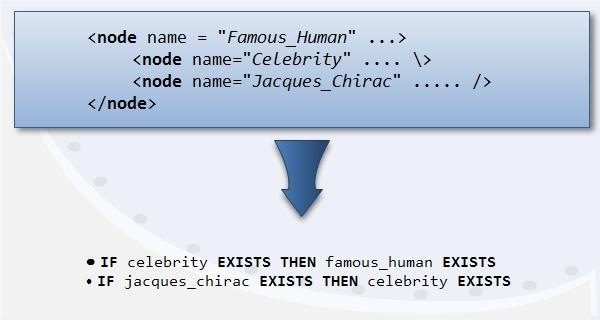
\includegraphics[scale=0.45]{graphics/contrib1::lscom_example}
			\caption{Extracting Fuzzy Rules from LSCOM Ontology}
			\label{lscom}
		\end{figure}

		\begin{figure}[h]
			\centering
			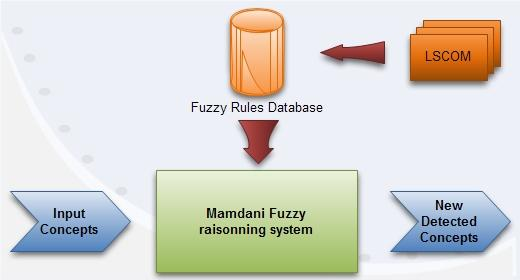
\includegraphics[scale=0.45]{graphics/contrib1::deduction}
			\caption{Deduction engine for situation refinement}
			\label{deduction}
		\end{figure}
		
		\subsubsection{Abduction engine}
		The abduction engine is based on a learning system that allows analysis of a  learning video database 
		in order to find possible relationships between concepts as input and expected concepts as output.
		These relationships are then considered  as fuzzy rules used for the deduction of new concepts based 
		on extracted ones from a test video database. Figure \ref{abduction} illustrates an overview of the abduction 
		engine.

		This engine uses the $\beta{}eta$ fuzzy systems (\emph{BFS}) based on a multi-agent genetic algorithm \citep{Kallel2006}.
		Thus, we use the equation \ref{genetic} for minimizing objective function $obj\_fun$ and then, 
		optimizing the learning process.
		
		Let $C$ be a set of $n$ concepts: $C = \{c_{1}, c_{2}, \dots, c_{n}\}$.
		And let $\mu'(c_{i})$ and $\mu''(c_{i})$ be two relevant degrees of the concept $c_{i}$ to a video content 
		respectively for generated concepts as output and the expected ones.
		We compute the objective function $obj\_fun$ by this equation:

		\begin{equation}
			\label{genetic}
			obj\_fun = \frac{\sum_{i=1}^{n} \Big(\mu''(c_{i}) - \mu'(c_{i})\Big)}{\sum_{i=1}^{n}(\mu''(c_{i}))^2}
		\end{equation}
		
		
		A similar abduction engine is described in \citep{Snoek2006} using \revAnglais{a} supervised \emph{SVM} classifier. 
		This latter consists in \revAnglais{analyzing} a set of concepts to discover potential relationships.

		We note that the output of \emph{level 2} is the fusion of two outputs from the deduction and abduction engines. 
		Eventual conflicting situation are treated in the same way as used in the \emph{level 1}. The degree of trust 
		for each reasoning engine is fixed by the fusion control process (\emph{level 4}).
		\begin{figure}[h]
			\centering
			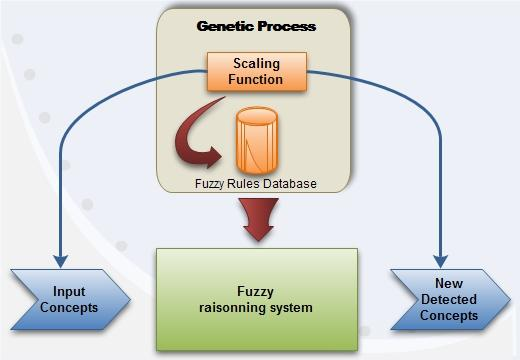
\includegraphics[scale=0.45]{graphics/contrib1::abduction}
			\caption{Abduction engine for situation refinement}
			\label{abduction}
		\end{figure}
		
	\subsection{Fusion Process Control (\emph{level 4})}
		This level aims at controlling the fusion process by manipulating trust  degree of each modality 
		(text, sound and images) and for each reasoning  engine (abduction and deduction). These trust degrees 
		are determined according to a supervised learning.

	We can conclude that the proposed multimodal fuzzy fusion is \revAnglais{characterized} \revAnglais{by} its ability to deliver 
	a rich and coherent semantic interpretation. This is mainly due to:
	\begin{itemize}	
		\item the use of fuzzy logic and fuzzy reasoning,
		\item a  maximum compatibility with the \emph{JDL/DFS} data fusion model,
		\item operating a maximum information  extracted from a video content (multimodality).
	\end{itemize}
	
	However, the quality of this fusion system is still dependent on the quality of initial semantic interpretations delivered by 
	unimodal analyzers.

	
	\subsection{Experimental Study}
		In order to illustrate the semantic enhancement of concept detection introduced 
		by our proposed fuzzy \revAnglais{fusion and} ontology-based framework, we have conducted two preliminary experiments 
		within two 
		multimedia evaluation campaigns. Hence, we expose the experimental setup and the 
		obtained results of our framework within \textsc{Trec} Video Retrieval Evaluation 2010 (\textsc{TrecVid 2010}) 
		\citep{Over2010} at the \textit{Semantic Indexing} task.
		

		\subsubsection{Datasets Description}
		We used datasets provided 
		in \textsc{TrecVid 2010} benchmark. The \textsc{TrecVid 2010} \textit{Semantic Indexing} task provides 
		two datasets proposed by the National Institute of Standards and Technology (\textsc{Nist}): 
		a test and a development dataset. 
		The development dataset (\emph{IACC.1.tv10.training}) contains $3200$ Internet Archive videos 
		($50GB$, $200 h$), while the test dataset (\emph{IACC.1.A}) contains approximately $8000$ Internet 
		Archive videos ($50GB$, $200 h$). The development dataset is annotated by $130$ semantic concepts.


		\subsubsection{Evaluation metrics}
		In order to be able to compare different indexing approaches, various system 
		effectiveness metrics have been used. These metrics are commonly based on precision
		(which is defined as the number of relevant answers as a part of the total number
		of retrieved ones), and recall (which is defined as the number of relevant answers
		as part of total relevant ones in the collection). In our experiments, we consider the following
		evaluation measures:  the \emph{Inferred Average Precision} (\textit{infAP}), the \emph{precision}
		(\textit{P}) and the recall (\textit{R}) as a
		performance metric for the \textsc{TrecVid 2010} \textit{Semantic Indexing} task.

		\subsubsection{Experiments with \textsc{TrecVid 2010} dataset}
		As an earlier experiment, we participated in \textsc{TrecVid 2010} 
		with two runs \textbf{\textit{$Regim_{4}$}} and  \textbf{\textit{$Regim_{5}$}} \citep{Elleuch2010}. 
		The first run integrates only a visual semantic concept detector using key-points detection 
		and visual features extraction tools \citep{Elleuch2010b}. And the second run aims at enhancing indexing 
		effectiveness of the first one through a rule based deduction reasoning engine.  
		Then, only the deduction process is used in the  \textbf{\textit{$Regim_{5}$}} run. 
		The abduction engine is ignored since a set of rules 
		\footnote{http://www-nlpir.nist.gov/projects/tv2010/tv10.semantic.indexing.relations2.txt} 
		were defined manually from the LSCOM ontology \citep{Kennedy2006}. 
		This rule list is based on two potential relationships between two concepts: 
		\emph{implies} (111 rules) and \emph{excludes} (5 rules). 
		For instance, the rule \textit{``Sky \textbf{implies} Outdoor''} depicts that if the concept 
		\textit{Sky} exists in a shot, then the concept \textit{Outdoor} exists too. 
		Similarly, the rule \textit{``Single\_Person \textbf{excludes} Crowd''} depicts that if the concept 
		\textit{Single\_Person} is detected in a shot, then the concept \textit{Crowd} doesn't exist.
		In our case, we \revAnglais{considered} only \textit{\textbf{implies}} relationships based rules.

		The results of both $regim_{4}$ and $regim_{5}$ are shown in figures \ref{res1tervcid2010} and
		\ref{trecvid20102}.
		The $regim_{5}$ run presents a concept detection enhancement over a classical visual concept 
		detector for concepts 6,  15 and 126 (respectively the concepts: \textit{Animal}, \textit{Boat\_Ship} and  
		\textit{Vehicle}). Further, the \textit{$regim_{5}$} run achieved an enhancement of $4.8\%$ for the mean inferred average
		precision (\textit{\textbf{infAP}}=$0.089$) among the \textit{$regim_{4}$} run (\textit{\textbf{infAP}}=$0.085$).
		Thus, having regard to a weak set of rules used in the deduction engine, 
		a knowledge based concept detection enhancement looks promising. Additionally, not all the concept set (130) 
		\revAnglais{were} considered in the rule list. 
		We would like also to point out that the \textsc{TrecVid 2010} evaluation process
		gave concept detection performances for only 30 concepts (among 130). 
		Thus, handling more concepts in the rule list should lead to a better semantic enhancement.

		\begin{figure*}[ht!]	
			\centering
			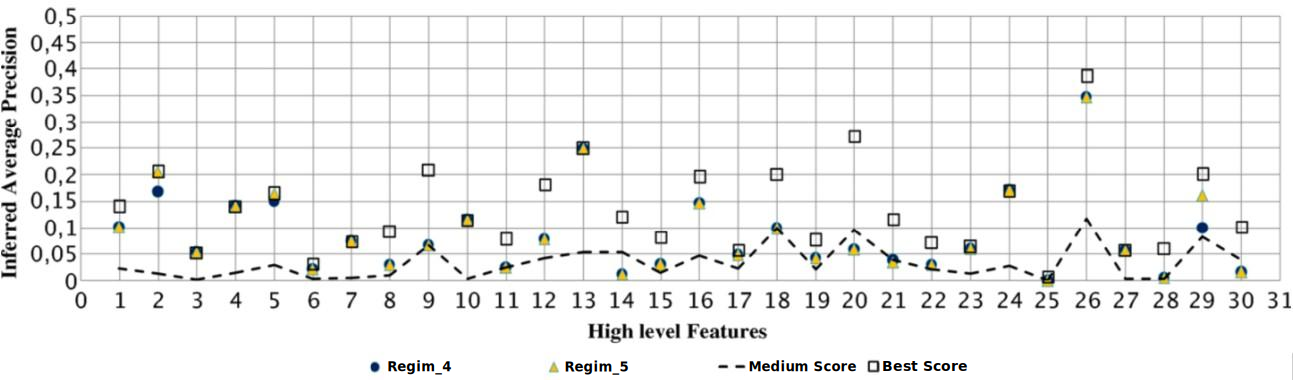
\includegraphics[width=\textwidth]{graphics/trecvid3}
			\caption{\textsc{TrecVid 2010}: $regim_{4}$ and $regim_{5}$ runs evaluations}
			\label{res1tervcid2010}
		\end{figure*}

		\begin{figure}[ht]
			\centering
			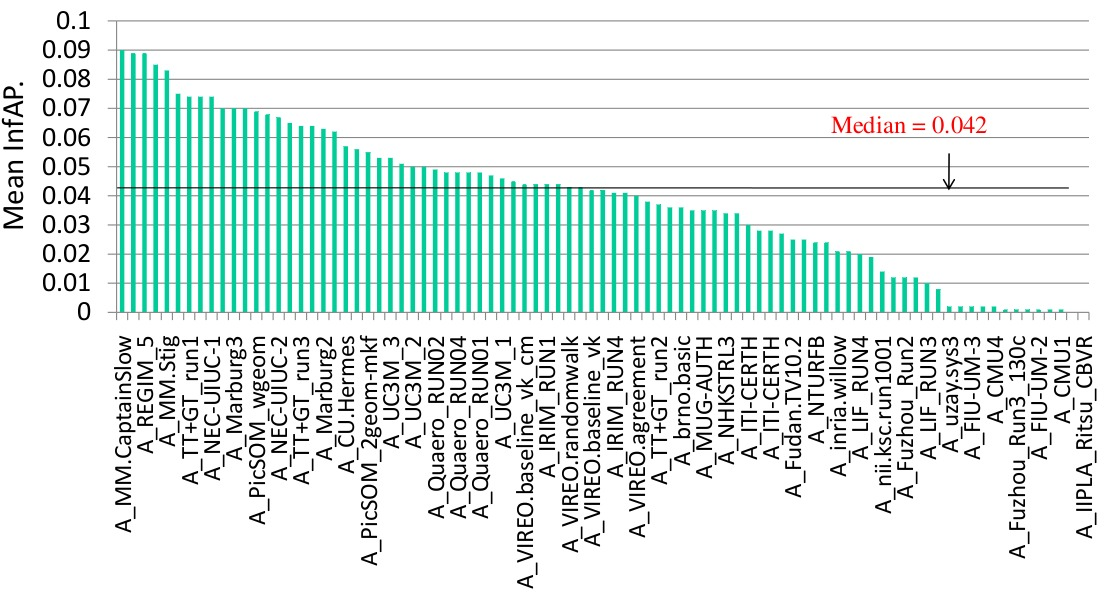
\includegraphics[scale=0.4]{figures/trecvid2010_2}
			\caption{\textsc{TrecVid 2010}: $regim_{5}$ ranking in  \textsc{TrecVid 2010} Semantic Indexing Task (SIN)}
			\label{trecvid20102}
		\end{figure}


		With such results, we extended our experimentation on the same dataset by using more rules 
		for the deduction engine. Indeed, the \textsc{Lscom} ontology is built on a set of semantic concepts
		interrelated by the generalization relationship (\textit{``is a''}). We transformed this 
		relationship into rules. In total, $4383$ rules \revAnglais{were} defined. The table \ref{tablscom} 
		shows some of these generated rules.

			\begin{table*}
				\centering	
				\caption{Sample rules extracted from the LSCOM ontology}
				\label{tablscom}
				\begin{tabular}{lcl} 
					
					\begin{small}\begin{sffamily}LSCOM Generalization Relationships\end{sffamily} 
					\end{small}& &
					\begin{small}\begin{sffamily}Extracted Rule\end{sffamily}\end{small} \\
					\hline
					\begin{small}\textit{Advocate \textbf{is a} Person} \end{small} & $\Longrightarrow$~~ &
						\begin{small}{\sffamily IsRelatedTo}(Advocate,Person)=1\end{small} \\
					\begin{small}\textit{Airport\_Terminal \textbf{is a} Building} \end{small} &  $\Longrightarrow$~~ &
						\begin{small}{\sffamily IsRelatedTo}(Airport\_Terminal,Building)=1\end{small} \\
					\begin{small}\textit{Backpack \textbf{is a} Luggage} \end{small} &  $\Longrightarrow$~~ &
						\begin{small}{\sffamily IsRelatedTo}(Backpack,Luggage)=1\end{small} \\
							
					\hline 
				\end{tabular}
			\end{table*}
		

		Obtained results are displayed in table \ref{lscom2}. Relying on these results, 
		we can conclude that an indexing system effectiveness can be clearly improved through 
		a knowledge-based approach. In fact, extracting and using rules from LSCOM ontology enable
		precision enhancement of about $18$\%. The recall is improved also of about $8$\%.

		\begin{table*}[h]
			\centering
			\caption{\textsc{TrecVid 2010}: Concept detection enhancement}
			\label{lscom2}
			\begin{tabular}{lp{1.2cm}p{1.2cm}p{1.2cm}p{1.2cm}p{1.2cm}p{1.2cm}}\hline
			\multicolumn{1}{c}{\multirow{2}{*}{\textit{\textbf{Semantic Concepts}}}} & \multicolumn{3}{c}{\textbf{Visual 				Concept Detector}}                                            & \multicolumn{3}{c}{\textbf								{LSCOM}}                                                                         \\ \cline{2-7} 
\multicolumn{1}{c}{}                                                     & \textit{\textbf{InfAP}}   & \textit{\textbf{P}}      & \multicolumn{1}{l|}{\textit{\textbf{R}}} & \textit{\textbf{infAP}}            & \textit{\textbf{P}}               & \textit{\textbf{R~~~~}}               \\ \hline
\multicolumn{1}{l|}{Outdoor}                                             & -                         & 0.52                     & \multicolumn{1}{c|}{0.59}                & -                                  & \textbf{0.88}                     & \textbf{0.77}                     \\
\multicolumn{1}{l|}{Vegetation}                                          & 0.1                       & 0.74                     & \multicolumn{1}{c|}{0.68}                & 0.1                                & 0.74                              & 0.68                              \\
\multicolumn{1}{l|}{Landscape}                                           & -                         & 0.6                      & \multicolumn{1}{c|}{0.79}                & -                                  & 0.6                               & 0.79                              \\
\multicolumn{1}{l|}{Sky}                                                 & -                         & 0.66                     & \multicolumn{1}{c|}{0.9}                 & -                                  & 0.66                              & 0.9                               \\
\multicolumn{1}{l|}{Trees}                                               & -                         & 0.62                     & \multicolumn{1}{c|}{0.72}                & -                                  & 0.62                              & 0.72                              \\
\multicolumn{1}{l|}{Mountain}                                            & -                         & 0.68                     & \multicolumn{1}{c|}{0.8}                 & -                                  & 0.68                              & 0.8                               \\
\multicolumn{1}{l|}{Ground\_Vehicle}                                     & 0.043                     & 0.3                      & \multicolumn{1}{c|}{0.66}                & \textbf{0.18}                      & \textbf{0.6}                      & \textbf{0.73}                     \\
\multicolumn{1}{l|}{Road}                                                & -                         & 0.43                     & \multicolumn{1}{c|}{0.6}                 & -                                  & 0.43                              & 0.6                               \\
\multicolumn{1}{l|}{Car}                                                 & 0.075                     & 0.42                     & \multicolumn{1}{c|}{0.64}                & \textbf{0.17}                      & \textbf{0.58}                     & \textbf{0.73}                     \\
\multicolumn{1}{l|}{Bus}                                                 & -                         & 0.52                     & \multicolumn{1}{c|}{0.73}                & -                                  & 0.52                              & 0.73                              \\
\multicolumn{1}{l|}{Bicycles}                                            & 0.142                     & 0.67                     & \multicolumn{1}{c|}{0.92}                & \textbf{0.185}                     & \textbf{0.82}                     & \textbf{0.97}                     \\
\multicolumn{1}{l|}{Emergency Vehicle}                                   & -                         & 0.9                      & \multicolumn{1}{c|}{0.83}                & -                                  & 0.9                               & 0.83                              \\
\multicolumn{1}{l|}{Building}                                            & 0.022                     & 0.18                     & \multicolumn{1}{c|}{0.22}                & \textbf{0.1}                       & \textbf{0.5}                      & \textbf{0.43}                     \\
\multicolumn{1}{l|}{Truck}                                               & -                         & 0.35                     & \multicolumn{1}{c|}{0.37}                & -                                  & 0.35                              & 0.37                              \\
\multicolumn{1}{l|}{Airplane Flying}                                     & 0.102                     & 0.8                      & \multicolumn{1}{c|}{0.78}                & 0.102                              & 0.8                               & 0.78                              \\
\multicolumn{1}{l|}{Airplane}                                            & -                         & 0.5                      & \multicolumn{1}{c|}{0.6}                 & -                                  & 0.6                               & 0.6                               \\ \hline\hline
\textbf{Total}                                                           & \multicolumn{1}{|l}{0.071}  & 0.53 & \multicolumn{1}{l|}{0.66}                & \multicolumn{1}{l}{\textbf{0.134}} & \multicolumn{1}{l}{\textbf{0.64}} & \multicolumn{1}{l}{\textbf{0.71}} \\ \hline
\end{tabular}
\end{table*}


		\subsection{Discussion}

		As discussed in the previous chapters, semantic concepts detection is based on the use of supervised 
		learning from manually annotated images samples. In fact, main approaches are almost exclusively focused 
		on an \revAnglais{independent} development of concept detectors which focuses on the extraction of low-level visual 
		features from positive and negative samples in order to \revAnglais{model} the high level concept. Nevertheless, 
		one semantic concept may appear and \revAnglais{exist} in many different contexts, further, its appearance and 
		meaning may be different according to these contexts. Thus, we think that concept based video indexing 
		is not optimal. Effectively, the indexing process requires a very big amount of training examples 
		in order to produce a generic indexing system, on the \revAnglais{one} hand, and slights the fact that concepts could 
		\revAnglais{exist} together, on the other hand. As an example, the semantic concept \emph{airplane\_{}flying} 
		coexists with the semantic concepts \emph{sky} and \emph{airplane}. Then, we can define the semantic 
		concept \emph{airplane\_{}flying} as context which makes a \revAnglais{relationship} between the concepts \emph{sky} 
		and \emph{airplane}. 

		The term \emph{context} is ambiguous. It \revAnglais{has} been defined in several ways. For the multimedia 
		community, a \emph{context} is introduced as an extra information for both concept detection 
		and scene classification \citep{Mylonas2005,Torralba2010}.

		To go further toward semantic enhancement, and considering both obtained results within 
		the \textsc{TrecVid 2010} and the research works focused on the semantic \emph{context}, 
		we attempted to introduce the \emph{context} in our proposed framework. Thus, we model 
		contextual information in order to better explore and understand a video content.
		In addition, we have opted for a standardized knowledge model for representing fuzzy relationships between
		semantic concepts. We have used then the ontologies 
		to model the fuzzy knowledge used to improve video indexing.
		
		As a next research step, we attempted to propose a context-based framework for video indexing.

	\section{Ontology based Framework for Video Content Indexing}
	\label{c1_2}

		The second revision of our fuzzy multi-modal framework leans on the introduction on the 
		\emph{context}, and the exploration of ontologies facilities to handle fuzzy relationships 
		between concepts. And for the new defined framework, we focused on: 1) semantic knowledge 
		representation and interpretation, and 2) \revAnglais{the} refinement process.

		Fuzzy knowledge representation intends to build the contextual space that \revAnglais{handles} relationships 
		among every context and its related semantic concepts. Such knowledge is extracted, modeled 
		and populated through an abduction engine mated with an inference engine. The latter is 
		provided by fuzzy description logics \citep{Straccia2006,Mantaras2015}. The fuzzy knowledge
		being extracted and populated within an ontology, the refinement process is used to enhance 
		the semantic interpretation of video indexing. Such a process is based on fuzzy rules used by 
		a deduction engine in order to infer new interpretation for a given \revAnglais{analyzed} video content.
		In the following, we detail our context based framework.

			\subsection{Framework Overview}
			In this section, we present the proposed fuzzy ontology-based framework 
			for reasoning in video indexing. The proposed approach involves two steps, 
			namely semantic knowledge representation/interpretation and refinement process.
			Our contribution is focused on modeling and building the context space and its 
			exploitation to enhance video indexing system.

			\begin{figure}[h]
				\centering
				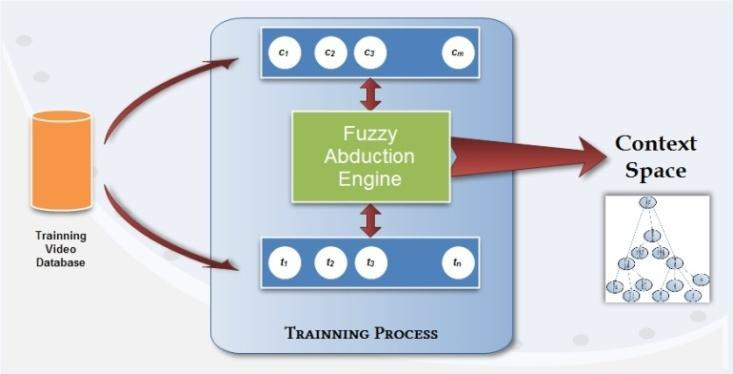
\includegraphics[scale=0.5]{graphics/contrib1::abduction2}
				\caption{The Context Based Fuzzy Abduction Engine}
				\label{abduction}
			\end{figure}
			
			In what follows, we display a description of both the semantic knowledge 
			representation/interpretation, then the refinement  process through the deduction engine.

				\subsection{Semantic Knowledge Representation/Interpretation}
				
				Based on a fuzzy Abduction Engine, the semantic knowledge representation and 	
				interpretation aims to analyze and model context spaces with fuzzy roles and rules 
				(by the same way as the first proposed framework \citep{Zarka2011}). These roles and 
				rules are used then, through firing a deduction engine, in order to discover further
				concepts and therefore enrich semantic interpretation.
			
				Therefore, a context-based ontology is, firstly, constructed  by populating different 
				relationships between each context and its semantic concepts, and secondly, providing 
				a deductive engine based on fuzzy rules in order to infer newer knowledge about a video content.

					\subsubsection{Extracting the Contextual Space} 
					The annotation process is used as semantic knowledge extraction tool to assist 
					experts to identify and define all semantic concepts involved in a domain 
					knowledge (context space). Generating such semantic knowledge has in recent 
					years been approached by collaborative efforts within multimedia retrieval 
					evaluation campaigns. 

					Thus, we propose an annotation approach to extract a semantic knowledge 
					for each context space. The following considerations are taken into consideration 
					for the proposed annotation \revAnglais{approach}:

						\begin{description} 
							\item[Unified lexicon:]  We adopt a fixed lexicon for annotation 
							of concepts and contexts in order to guarantee a convergence in 
							user assigned free labels. The \textsc{LsCom} ontology includes a 
							unified set \revAnglais{of} concepts. We used then the \textsc{LsCom} provided 
							lexicons to define concepts (\textbf{eg.} \textit{Sky, Airplane, 
							Road}) and contexts (\textbf{eg.} \textit{ Office, 
							Airplane\_Flying, Urban}),
							
							\item[Soft annotation:] Concept/context relationships can be considered 
							as uncertain. Fuzzy relationships should be then used for the
							annotation approach. A membership relevance degree is then 
							attributed to a semantic concept and a target context. We propose 
							so three relevance levels, namely\textit{ “Relevant”}, 
							\textit{“Not-Relevant”} and \textit{“Not-Exist”}.  
							\textit{“Relevant”}, \textit{“Not-Relevant”} respectively indicate 
							that the concept is present and semantically strong (weak) in the 
							target context and \textit{“Not-Exist”} their lack. 
						\end{description} 

					\subsubsection{Ontology Structure}  
						A less expressive fuzzy description logic is used to describe the 
						semantic knowledge. Such a choice is argued to facilitate fast computation.

						In the following, we display how we model and populate a contextual knowledge 
						for semantic interpretation.

						Our fuzzy ontology is modeled as:
						$O^{f} = \{T, C, R^{f}_{tc}, R^{f}_{ct}, R^{f}_{cc}, Q\}$, 
							where : 
							\begin{itemize} 
							\item $T = \{t_{1}, t_{2}, ..., t_{n}\}$ is a set of $n$ contexts; 
							\item $C = \{c_{1}, c_{2}, ..., c_{m}\}$ is a set of $m$ concepts; 
							\item $R^{f}_{t_{i}c_{j}} : TxC  \rightarrow [0,1], i 
								\in \{0, ..., n\}~and~j \in \{0, ..., m\}$ is a 
								fuzzy role between context $t_{i}$ and concept $c_{j}$; 
							\item $R^{f}_{c_{i}t_{j}} : CxT  \rightarrow [0,1], i 
								\in \{0, ..., m\}~and~j \in \{0, ..., n\}$ is a 
									fuzzy role between concept $c_{i}$ and context $t_{j}$; 
							\item $R^{f}_{c_{i}c_{j}} : CxC \rightarrow [0,1], ~~ i, j 
								\in \{0, ..., m\}$ is a 
								fuzzy role between concept $c_{i}$ and concept $c_{j}$ ;		 
							\item $Q$ is a set of fuzzy qualifier. In $O^{f}$, 
							we define two qualifiers: \textit{“weak”} and \textit{“strong”}. 
							\end{itemize} 
						We define too sub-roles between contexts and concepts: 
						\{\textit{Generalization, IsRelatedTo, IsPartOf, Includes}\}. 
						The interpretation of these roles is detailed in the Table \ref{table1.1}. 
						\begin{table}[h!] 
							\caption{Semantic Relationships Between Concepts and Contexts} 
							\label{table1.1} 
							\begin{center} 
							\begin{footnotesize} 
							\begin{tabular}{c|c|c|c|c} 
								\hline\textbf{ \textit{Name}} & \textbf{\textit{Symbol}} & 
								\textbf{\textit{Meaning}} & \textbf{\textit{Type}} & 
								\textbf{\textit{Definition}} \\ 
					
								\hline Generalization & $t_{i}:t_{j} $ & 
								The concept $c_{i}$ is the generalization of the concept $c_{j} $ 
				 				&  $TxT$  & LSCOM \\ 
								
								\hline IsRelatedTo 	& $c_{i} |t{k}\rightarrow c_{j}$ &
								The concept $c_{i}$ is related to the concept $c_{j}$ within $t_{k}$ 
				 				& $CxC$  & Learning \\ 
					
								\hline IsPartOf 	& $\{c_{i}\} \in t_{j}	$ & 
								A set of concept $c_{i}$ is a part of the context $t_{j}$ 
								& $CxT$ & Learning \\ 
					
								\hline Includes 	& $t_{i} \supset c_{j}$	& 
								The context $t_{i}$ includes the concept $c_{j}$ 
				 				&  $TxC$ & Expert \\ 
								\hline 
							\end{tabular} 
							\end{footnotesize} 
							\end{center} 
						\end{table} 

						\begin{itemize}
							\item \textit{\textbf{Generalization Role}}: The \textit{``generalization''} 
							role between $t_{i}$ and $t_{j}$ is defined if $t_{i}$ 
							is a sub-context of $t_{j}$, 
							which is denoted as: $t_{i}:t_{j} $.  As an example, \textit{“Ground\_Vehicle”}
							and \textit{“Vehicle”} are related as \textit{“Generalization”} relationship.
							\textit{Ground\_Vehicle} : \textit{Vehicle} indicates that all relevant video
							shots for sub-context \textit{“Ground\_Vehicle”} must also be relevant to context
							\textit{“Vehicle”}. The generalization relationship is the most common relation
							used to build ontology hierarchy, which can be exploited to enhance concept
							detectors. The LSCOM  ontology, dealing only with this relationship, 
							provides a ready enumeration of generalizations between all defined concepts. 
			
							\item \textit{\textbf{IsRelatedTo Role}} The \textit{“IsRelatedTo”} 
							role between $c_{i}$ and $c_{j}$ is defined if $c_{i}$ is related
							to $c_{j}$ within $t_{k}$ , which is denoted as: $c_{i} |t{k}\rightarrow 
							c_{j}$. As an example, \textit{ “Snow”} and \textit{“Mountain”} are 
							related  as \textit{“IsRelatedTo”} relationship. $Snow |Landscape 
							\rightarrow Mountain$ suggests that the all relevant video shots 
							to concept \textit{“Snow”} within the context \textit{“Landscape”} 
							could be relevant to concept \textit{“Mountain”}. 
		 
							\item \textit{\textbf{IsPartOf Role}} The \textit{“IsPartOf”} role between
							$c_{i}$ and $t_{j}$ is defined if $c_{i}$  is part of $t_{j}$, 
							which is denoted as:  $\{c_{i}\} \in t_{j}$. As an example, 
							{\textit{“Sky”, “AirPlane”}} and \textit{“AirPlane\_Flying”} are related 
							as \textit{“IsPartOf”} relationship. \textit{Sky, AirPlane $\in$  
							AirPlane\_Flying} lead to all relevant video shots to concept 
							\textit{“Sky”} and \textit{“Airplane”} could be relevant to 
							context \textit{“AirPlane\_Flying”}. 

							\item \textit{\textbf{Includes Role}} The \textit{“Includes”} role 
							between $t_{i}$ and $c_{j}$ is defined if $t_{i}$ includes $c_{j}$, 
							which is denoted as: $t_{i} \supset c_{j}$. As an example, 
							\textit{“CarRacing”} and \textit{“Car”} are related as 
							\textit{“Includes”} relationship. \textit{“CarRacing” 
							$\supset$ “Car”} suggests that the all relevant video shots 
							to context\textit{ “CarRacing”} could be relevant to concept \textit{“Car”}. 
						\end{itemize}

						In order to enable handling real world situations, we introduced for every defined
						role a degree of confidence $\alpha$ where $\alpha \in [0,1]$.
						In addition, for each role, a $\mu$ function is defined that aims 
						to \revAnglais{compute} respectively for each related pairwise $\textless c_{i},c_{j}
						\textgreater$, $\textless c_{i},t_{j}\textgreater$ and $\textless t_{j},c_{i}
						\textgreater$ a degree that $c_{i}$ supplied for $c_{j}$, $c_{i}$ supplied 
						for $t_{j}$ and $t_{j}$ supplied for $c_{i}$. $\alpha$ and $\mu$ are generated
						automatically through Abduction Engine based on $\beta$eta function \citep{Aouiti2003}. 
						Generally, the $\beta$eta function is defined as follows: 
						\begin{equation} 
							\beta(x) = 
							 \left\{ 
		   					\begin{array}{cr} 
		     						(\frac{(x-x_{0})}{(x_{c}-x_{0})})^{p} (\frac{(x_{1}-x)}
								{(x_{1}-x_{0})})^{q}&if~x \in [x_{0}, x_{1}] \\ 
		    						 0 & otherwise \\ 
		   					\end{array} 
		 					\right. 
						\end{equation} 
						Where: 
						\begin{itemize} 
							\item $p > 0, q > 0$; 
							\item $x_{0}$ and $x_{1}$ are real parameters; 
							\item $x_{c} = \frac{(px_{1}+qx_{0})}{(p+q)}$. 
						\end{itemize} 
		 
						According to relevance degrees proposed in our context annotation 
						framework, our fuzzy ontology $O^{f}$ employs two qualifiers 
						($Q = \{Weak, String\}$), in order to provide a fine-tuning 
						of degrees of confidence. Thus, each rule is
						\textit{“Strong”} qualified if its degree of confidence 
						is greater than 0.5, else \textit{"Weak"} qualified. 
		

	\subsubsection{Building ontology through Abduction Engine} 
			In order to detect and extract further rules within concepts and contexts, 
			we use the Multi-Agent Genetic Algorithm for the Design 
			of $\beta$eta Fuzzy Systems (\textsc{Magad-Bfs}), proposed in \citep{Kallel2006}, as an Abduction Engine. 
			 
			Based on genetic algorithm (\textsc{Ga}), \textsc{Magad-Bfs} allows optimizing a fuzzy logic system 
			(\textsc{Fls}) with Beta membership functions \citep{Alimi2000}. It consists of minimizing
			the number of $\beta$eta fuzzy rules $N_{R^{f}}$, which are formulated according to 
			the equation \ref{eq2}, while adjusting $\beta$eta function $p$ and $q$ parameter’s ($obj_{fun}$) 
			of each rule until a desired precision $\epsilon$. 
			 
		\begin{equation} 
			\label{eq2}
			R_{j}: \{ R_{ct}^{f}, R_{cc}^{f}, R_{tc}^{f}\}:~IF~ (X~is~Q^{j})~THEN~(Y=f_{i}(X)) 
		\end{equation} 
		 
		Where: 
		\begin{itemize} 
			\item $X = C\cup T$ is an input variable; 
			\item $Y = C\cup T$ 	is an output variable; 
			\item $Q^{j}$ is a linguistic qualifiers of input variable; 
			\item $f_{j}$ is the output of the $j^{th}$ fuzzy rule. 
		\end{itemize} 
		 
		The objective function ($obj_{fun}$) to be minimized is defined as follows: 
		\begin{equation} 
			f^{*}(X)=[\sum_{j=1}^{N_{R^{f}}} f_{j}(X)\beta_{j}(X)] 
		\end{equation} 
		 
		\begin{equation} 
		obj_{fun} = \frac{\sum_{i=1}^{m+n} [Y_{i}-f^{*}(X_{i}) ]^{2}}{\sum_{i=1}^{m+n} Y_{i}^{2} } * 
		(\frac{N_{R^{f}} - N_{min} }{N_{max} - N_{min} + 1}) 
		\end{equation} 
		Where: 
		\begin{itemize} 
			\item $N_{min}$ and $N_{max}$ are respectively the minimum and the maximum number of fuzzy rules allowed in the 
			final $\beta$eta fuzzy system; 
			\item $\mu_{j}=\beta_{j}$ is a $\beta$eta function that \revAnglais{activates} the $j^{th}$ fuzzy rule. 
		\end{itemize} 
		 

		\subsubsection{Deduction engine}
		In the indexing process, each video shot $V_{S_{k}}$ is ranked with a probabilistic measure
		$P(V_{S_{k}}|c_{i})$ or  $P(V_{S_{k}}|t_{j})$. 
		Based on the latter scores, a fuzzification step is 
		performed. The latter aims to handle the imprecision and inexactness of concepts and contexts detectors, on one hand, 
		and generate the fuzzy inputs required by fuzzy rules on the other hand. Thus, we consider a concept $c_{i}$ 
		or a context $t_{j}$ \textit{“Relevant”} in a video shot $V_{S_{k}}$ if $P(V_{S_{k}}|c_{i})$ respectively $P(V_{S_{k}}|t_{j})$  is grant than $0.7$. However\revAnglais{,} a concept or a context 
		is qualified by \textit{“Not-Relevant”} in a video shot $V_{S_{k}}$ if  $P(V_{S_{k}}|c_{i})$ respectively $P(V_{S_{k}}|t_{j})$ is between $0.3$ and $0.7$. 
		 
		Based on these fuzzy inputs, the deduction engine explores all defined rules in order to infer the most appropriate one and 
		thus generates an optimal score for the target rule output. In this \revAnglais{field}, two cases arise: when a fuzzy rule is \textit{“Strong”} qualified or \textit{“Weak”}. 
		 
		In the first case, the deduction engine proceeds as follow: Let $R^{f}_{k}$  a fuzzy rule defined as :$R^{f}_{k}$: $c_{i}$ is \textit{Strong RelatedTo} $c{j}$ within $t_{k'}$ and let $P(V_{S_{i}}|c_{i})$ and  $P(V_{S_{i}}|t_{k'})$, respectively, a score detection of concept $c_{i}$ and context $t_{k'}$ in the same video shot $V_{S_{i}}$. The optimal score, or the deduced relevance degree, of the fuzzy rule $R^{f}_{k}$ outputs, denoted as $\alpha'_{k}(c_{j})$, is computed as follow: 
		\begin{equation} 
			\alpha'_{k}(c_{j})=\mu_{k}*(max\{P(V_{S_{k}}|c_{i}),P(V_{S_{i}}|t_{k'})\})*\mu_{Strong}(\alpha_{k}) 
		\end{equation} 
		Where $\mu_{k}$ and $\alpha_{k}$ are, respectively, the $\beta$eta membership function and the confidence degree of the $k^{th}$ fuzzy rule according the role \textit{“IsRelatedTo”}. 
		 
		In the second case, the deduction engine applies the following equation. 
		\begin{equation} 
			\alpha'_{k}(c_{j})=\mu_{k}*(min\{P(V_{S_{k}}|c_{i}),P(V_{S_{i}}|t_{k'})\})*\mu_{Weak}(\alpha_{k}) 
		\end{equation} 
		The same approach is built by the deduction engine for the other rules according the role \textit{“IsPartOf”}, \textit{“Includes”} and \textit{“Generalisation”}. 

	\subsection{Fuzzy Ontology Construction}
		 As aforementioned, fuzzy contextual ontology is a formal and explicit representation 
		of semantic knowledge in visual domain. In this section, we will detail its implementation process.
		
		\subsubsection{Knowledge extraction}
		In order to build the context space, a large-scale corpus is requested for generalizing
		contextual information and relationships between contexts and concepts. Thus, 
		we explored the development \revAnglais{data} set provided by the evaluation campaign \textsc{TrecVid}
		\textsc{IACC.1.Tv10.Training2} which is composed of $119~685$ shots. Each shot is manually
		assigned to a predefined context specifying the meaning of its contents recognized by experts. 
		
		\subsubsection{Fuzzy Rules Abduction}
		In the aim to discover fuzzy rules in the form of \textit{“Includes”}, \textit{“IsPartOf”} 
		and \textit{“IsRelatedTo”}, the abduction engine is trained by the use of the semantic
		knowledge. Thus, for every output of the above enumerated roles, feature vectors are 
		firstly generated.  A feature vector is a string of numerical values whose dimension
		is  $n + m$ that correspond to the number of concepts and contexts. 

		A $1$ or $0.5$ or $0$, at $i^{th}$ position, indicates, respectively, whether 
		the $i^{th}$ concept or context is \textit{“Relevant”} ($1$), \textit{“Not-Relevant”} 
		($0.5$) or \textit{“Not-Exist”} ($0$) for the expected output. Then, the abduction engine is 
		consecutively learned and provides fuzzy rules by estimating the 
		degree of confidence $\alpha$ and the $\beta$ membership function $\mu$, as shown in Table \ref{tabb2}.

	
		\begin{table*}
				\centering	
				\caption{A Partial view of the abducted Fuzzy rules}
				\label{tabb2}
				\begin{tabular}{c|l|c|c} 
					\hline
					\begin{small}\begin{sffamily}Name\end{sffamily} \end{small}& 
					\begin{small}\begin{sffamily}The abducted fuzzy rule\end{sffamily}\end{small} &
					\begin{small}\begin{sffamily}Qualifier\end{sffamily}\end{small} &
					\begin{small}\begin{sffamily}$\beta$eta membership function\end{sffamily}\end{small} \\
					\hline

					\begin{small}Generalization\end{small}&
					\begin{small}$Airplane\_flying : Vehicule$\end{small}&
					\begin{small}Strong\end{small}&
					\begin{small}-\end{small}\\
							
					\hline 

					\multirow{4}{*}{\begin{small}Generalization\end{small}}&
					\begin{small}$Airplane~|~Airplane\_flying \longrightarrow  sky$\end{small}&
					\begin{small}Strong\end{small}&
					\begin{small}$p=10$, $q=0.01$\end{small}\\

					& 
					\begin{small}$Snow~|~Landscape \longrightarrow  Moutain$\end{small}&
					\begin{small}Weak\end{small}&
					\begin{small}$p=0.01$, $q=1$\end{small}\\

					& 
					\begin{small}$\{Snow, Mountain\}~|~Landscape \longrightarrow  Sky$\end{small}&
					\begin{small}Strong\end{small}&
					\begin{small}$p=11$, $q=0.1$\end{small}\\
					
					& 
					\begin{small}$Person~|~Studio\_News \longrightarrow  Anchorperson$\end{small}&
					\begin{small}Strong\end{small}&
					\begin{small}$p=8$, $q=0.03$\end{small}\\
							
					\hline 
	
					
					\multirow{2}{*}{\begin{small}IsPartOf\end{small}}&
					\begin{small}$\{sky,Trees\} \in Landscape$\end{small}&
					\begin{small}Strong\end{small}&
					\begin{small}$p=8$, $q=0.01$\end{small}\\

					& 
					\begin{small}$\{Building,Sky,Road,Car\} \in Urban$ \end{small}&
					\begin{small}Strong\end{small}&
					\begin{small}$p=9$, $q=0.02$\end{small}\\

					\hline 

					\begin{small}Includes\end{small}&
					\begin{small}$Landscape  \supset Snow$\end{small}&
					\begin{small}weak\end{small}&
					\begin{small}$p=2$, $q=2$\end{small}\\

					\hline 
				\end{tabular}
			\end{table*}

	\subsection{Experiments}

		In this section, we discuss the obtained results for an experiment that we conducted on 
		\textsc{TrecVid 2010} dataset. The latter dataset is widely employed for the evaluation 
		of video semantic indexing accuracy.
	
		The main goal of our experiment is to evaluate the use of the context space for semantic 
		concept detection and to evaluate the effectiveness of our proposed knowledge based 
		approach compared to existing techniques.

		At first, we evaluate the effectiveness of the use of a semantic knowledge induced 
		by the proposed fuzzy contextual ontology to enhance the detection of semantic concepts 
		and to better enhance the semantic interpretation of a video content. Thus, we use the 
		following metrics:  \textit{inferred average precision} (\textit{infAP}), the 
		\textit{precision} (P) and the \textit{recall} (R). 

		By the use of the contexts defined in figure \ref{contextes}, we obtained results reported in table \ref{tab3}.

		\begin{figure}[ht!]	
			\centering
			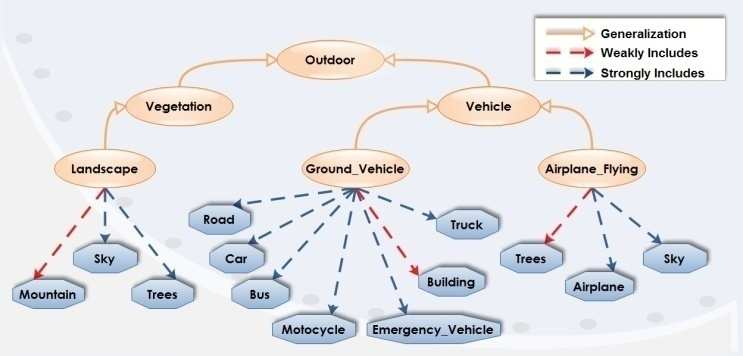
\includegraphics[width=\textwidth]{graphics/contextess}
			\caption{Partial view of concept distribution generated by contextual experts annotation}
			\label{contextes}
		\end{figure}



		\begin{table*}[h]
			\centering
			\caption{\textsc{TrecVid 2010}: Concept retrieval performance for different Concept detection methodologies}
			\label{tab3}
			\begin{tabular}{l||ccc|ccc|cc}\hline


				\multirow{2}{*}{\textit{\textbf{Semantic Concepts}}} & 
				\multicolumn{3}{c}{\textbf{Concept Detector}} & 
				\multicolumn{3}{c}{\textbf{LSCOM}}&
				\multicolumn{2}{c}{\textbf{$O^{f}$}}\\ 

				& infAP & P & R & infAP & P & R & P & R\\
				\hline
				\hline
	
Outdoor	&	-&	0.52&	0.59&	-&	\textbf{0.88}	& \textbf{0.77} & \textbf{0.9} & \textbf{0.82}\\
Vegetation	& 0.1 	& 0.74& 0.68& 0.1& 0.74 & 0.68 & \textbf{0.93} & \textbf{0.87} \\
Landscape& -& 0.6& 0.79& -& 0.6 & 0.79& \textbf{0.7} & \textbf{0.82}\\
Sky& -& 0.66& 0.9& -& 0.66& 0.9 & \textbf{0.85} & \textbf{0.95} \\
Trees& -& 0.62& 0.72 & - & 0.62 & 0.72 & \textbf{0.73} & \textbf{0.82}\\
Mountain& -& 0.68 & 0.8 & -  & 0.68 & 0.8 & \textbf{0.83} & \textbf{0.85} \\
Ground\_Vehicle& 0.043  & 0.3& 0.66& \textbf{0.18} & \textbf{0.6} & \textbf{0.73} & \textbf{0.69} & \textbf{0.75}\\
Road& -& 0.43& 0.6 & -& 0.43& 0.6 & \textbf{0.88} & \textbf{0.9} \\
Car  & 0.075 & 0.42 & 0.64& \textbf{0.17} & \textbf{0.58} & \textbf{0.73} & \textbf{0.79} & \textbf{0.83}\\
Bus& -& 0.52& 0.73& - & 0.52& 0.73 & 0.52 & 0.73\\
Bicycles& 0.142& 0.67& 0.92& \textbf{0.185}& \textbf{0.82}& \textbf{0.97} & \textbf{0.83} & 0.97\\
Emergency Vehicle& -& 0.9& 0.83& - & 0.9& 0.83 & 0.9& 0.83\\
Building& 0.022& 0.18& 0.22& \textbf{0.1}& \textbf{0.5}& \textbf{0.43} & \textbf{0.55} & \textbf{0.45} \\
Truck & -& 0.35& 0.37& -& 0.35& 0.37 & 0.35 & 0.37\\
Airplane Flying & 0.102& 0.8 & 0.78& 0.102& 0.8& 0.78 & \textbf{0.83} & \textbf{0.79}  \\
Airplane  & -& 0.5& 0.6& -& \textbf{0.6}& 0.6  & \textbf{0.71} & \textbf{0.69}\\
\hline
\end{tabular}
\end{table*}

	\revAnglais{As} displayed in table  \ref{tab3}, the video indexing accuracy is clearly improved when a knowledge-based approach is used. In fact, when the \textsc{LsCom} ontology is used, the precision improvement of semantic concept detection in the order of $11\%$. However, we obtained $21\%$ through the use of $O^{f}$ ontology. This improvement is mainly due to the hierarchical roles of each one. 


	The \textsc{LsCom}  ontology, based on \textit{“Generalization”} roles,
 provides enrichment only for the concepts of a higher
 level. However, the $O^{f}$ ontology expounds other roles
 such as \textit{“IsPartOf”}, \textit{“Includes”} and \textit{“IsRelatedTo”}.
 These allow us to highlight the relation between a
 context and its concepts and concept-concept within a
 target context space.


	The proposed approach improves not only the precision
 of contexts detection, but also concepts detection. In
 fact, our ontology $O^{f}$ performs best for 16 (6 context
 and 10 concepts) for 17 high level feature. This result is
 rather obvious: the proposed ontology $O^{f}$  tries to
 represent the context space; with 4 roles
 (\textit{“Generalization”},
 \textit{“IsPartOf”},
 \textit{“Includes”}
 and
 \textit{“IsRelatedTo”}); by using an Abduction Engine. The
 latter automatically generates fuzzy rules and optimizes
 them. These fuzzy rules, that represent the ground truth,
 further improve the effectiveness of video indexing
systems. In addition, we note that using the deduction
 engine has improved the ranking of video shot results,
 which will improve the Inferred Average Precision.
 The context-based concept fusion framework enhances
 the high level feature detection. In fact, the recall is
 improved for $5$ (Outdoor, Vegetation, Vehicle,
 Ground\_Vehicle, Airplane-Flying) out of $17$ high level
 feature. We can see that the enrichment has only
 targeted the context. Although this recall improvement (about $2\%$), the precision improvement has declined.
 
	\subsection{Discussion}
	The experiments that we conducted indicate clearly that semantic concepts could be efficiently 
	detected when a knowledge-based approach is incorporated within a video indexing system. Thus, 
	the core contribution of this work is the \revAnglais{implementation} of a fuzzy contextual ontology. 
	
	\revFaiz{In fact, the first experiment dealt with the \textsc{LsCom} as a knowledge back-end 
	for the deduction engine. The obtained result showed that such knowledge-based approach 
	could deduce and detect further semantic concepts. Then, the proposed context-based fuzzy 
	ontology $O^{f}$ defined fuzzy semantic relationships between semantic concepts and 
	semantic contexts. This ontology showed better and promising result.}


	Nevertheless, the latter aims to model knowledge of concepts which are extracted from a 
	valuable data-source through an abduction engine. Generally, video annotation tools provide
	as outputs valuable information about semantic interpretation for video content 
	\citep{Dasiopoulou2011}. In literature, the available annotation tools \revAnglais{do} not support
	contextual information during the annotation process. In the next section, we display our
	proposed context-based video annotation tool.




	\section{Collaborative Annotation}
	\label{c1_3}

	The next proposition aims to improve the video annotation results through the 
	contextual information \citep{Ksentini2012}. Then, we focus on the collaborative
	annotation through sharing the past annotations in the aim to manage conflict situations.
	Also, we introduce semantic contexts in the annotation process in order to provide answers
	to the sensorial problem: one concept can present different meaning within different contexts.
	
	\subsection{Collaborative Annotation}
		
	The collaborative aspect of the proposed annotation tool aims to promote annotation
	sharing between annotators while being guided by visual tools a better annotate images.
	In order to assist the annotator for better video semantic comprehension, we integrate the following tools.

	\begin{description}

		\item[Detection shots of key frames:] is a tool that \revAnglais{makes} it possible to add useful 
		information for image annotation, and to better identify the context in which the objects
		appeared, either by listening \revAnglais{to} the sound track or the follow-up of object movements. 
		From the video descriptions, we recovered the temporal position of the key frame to annotate, 
		the time beginning of the representative plan and its duration.

		\item[Sharing passed interpretations by other annotators:] we think that it is very important 
		to manage conflicts which can occur. For instance, for a given image, an annotator can refer 
		to the previous annotations presented in chronological order in order to take idea and then 
		to correctly annotate the image. We estimate inter-annotator agreement in order to manage
		conflicting situations.

		\item[Automatic suggestion of concepts:] The annotation tool \revAnglais{suggests} to the user some concepts
		related to choses ones. The suggestion is made by a statistical \revAnglais{study} that we conducted 
		on annotated datasets delivered by \textsc{TrecVid2010}. In fact, these statistical studies 
		\revAnglais{look} for inter-concepts co-occurrence. Then, and when the annotator \revAnglais{chooses} a concept for 
		a given image, the annotation tool looks for co-occurred concepts in order to suggest 
		them to the annotator. 

		\item[Ontology driven annotation:] generally, the annotation tools use informal annotation
		(either binary or free texts). In our proposed annotation tool, we propose to integrate an 
		annotation controlled using concepts from the \textsc{LsCom} ontology in order to have a formal 
		and standard annotation. The ontology used is presented by a tree structure which allows to
		the annotators to traverse the concept list and select pertinent ones efficiently.
	\end{description}

	The figure \ref{annotation_tool} illustrates the proposed annotation tool.

	\begin{figure}[ht!]	
		\centering
		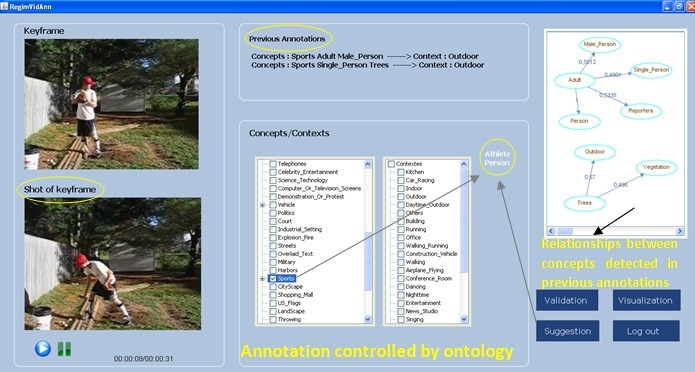
\includegraphics[width=\textwidth]{graphics/annotation_tool}
		\caption{Overview of the proposed Collaborative Annotation Tool}
		\label{annotation_tool}
	\end{figure}


	\subsection{Conceptual Relationship Mining}

	In order to estimate the conceptual relationships between the concepts detected during
	the annotation process, we represent them by characteristic vectors. Then , we calculate
	the inter-concepts similarities. These vectors are defined by analyzing the final results
	of the video annotation process. Thus, we define a dynamic matrix whose lines represent
	the annotated key-frames, and the columns \revAnglais{of} the annotated concepts.  

	As concepts have various appearances according to the context in which they appear, 
	we propose to add the notion of context in our calculations of conceptual relationships.
	Since the similarity between two concepts $C_{i}$ and $C_{j}$ varies from a context to another, 
	we extract from the initial matrix sub-matrices. Each one of the \revAnglais{latters} represents the 
	frequencies of concept appearances in the images in a \revAnglais{well-defined} context.

	Once the vectors are defined, we calculate the similarity between the concepts by adopting 
	the similarity measure \emph{Cosine} Similarity. This latter is frequently used as a measurement
	of resemblance between two objects. Thus it is defined as follows:
		\begin{equation}
				cosine(c,d) = \frac{\vec{C_{i}} . 
				\vec{C_{j}}}{|C_{i}| . |C_{j}|}
		\end{equation}

	\subsection{Visualization}

	The conceptual relations withdrawn in the preceding section do not make it possible 
	to appreciate in an easy way the similarity between the concepts. It is thus preferable
	to have a comprehensive view of these semantic relations for better assimilating them.  
	The generated visual graph comprises a set of nodes and a set of undirected arcs \revAnglais{that} respectively
	represent the semantic concepts and semantic relationships \ref{annotation_tool2}. 

	In order to emphasize the notion of context, we propose to divide the contextual graph 
	into sub-graphs of which each one represents the conceptual relationships between the concepts in a given context.
	\begin{figure}[ht!]	
		\centering
		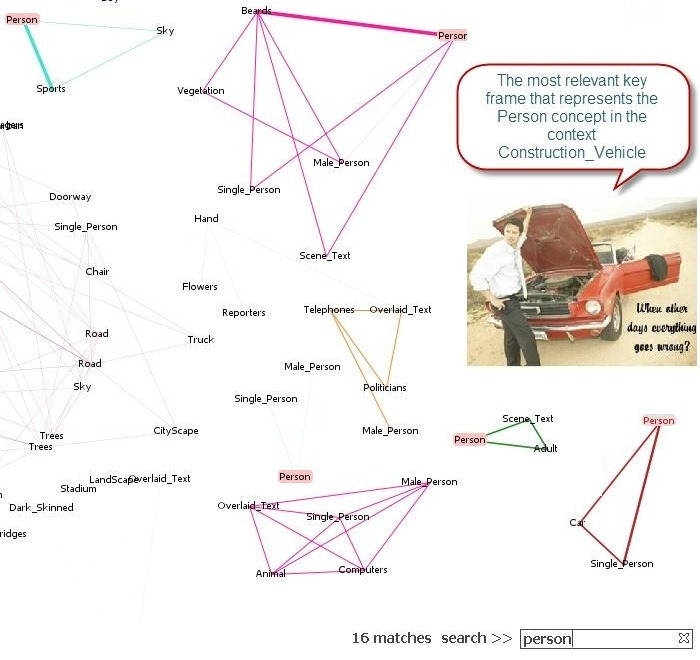
\includegraphics[scale=0.5]{graphics/annotation_tool2}
		\caption{Visualization of Conceptual Relationships}
		\label{annotation_tool2}
	\end{figure}

	\subsection{Discussion}

	The proposed collaborative annotation tool \revAnglais{delivers} an annotated dataset where each 
	image/shot is tagged by a set of semantic concepts/contexts. Based on such annotation outputs, 
	we conducted then an earlier statistical study on concepts co-occurrence. 
	We obtained then interesting relationships that could be considered as valuable knowledge. 
	Indeed, the relationship between contexts and concepts \revAnglais{cannot} be revealed directly 
	through annotated images/shots. We believe that such valuable knowledge is crucial to 
	enhance multimedia content indexing: given a defined context in an image and 
	inter-relationships between concepts within that context, the detection of a concept may 
	lead to deduce the existence of other concepts. The importance of this knowledge to improve 
	the indexing performance is detailed in the next chapter. 
	

\section{Conclusion}
\label{c1_4}
	In the present chapter, we presented our  first proposition for a contextual 
	knowledge based framework for enhancing a semantic interpretation about a multimedia
	content. The proposed framework deals with rich semantic structure in order to model
	many information in relation to semantic concepts and their interrelationships. 
	
	Our framework effectiveness and performance were proved on a multimedia benchmark 
	(\textsc{TrecVid 2010}). The effectiveness of our knowledge based framework, 
	in terms of precision and recall, is proved on diverse concepts.
	
	%Future works should consider of extending other knowledge sources such as 
	\textsc{Flickr} images. 
	In the next chapter, we investigate more work  
	on the automation of the abduction engine, and modeling a generic ontology
	structure in order to handle various information from various fields.

		




			\chapter{Fuzzy Context-Based Ontology Generation Framework for Reasoning in Multimedia Content}
\label{c2}
	In this chapter, we discuss the second contribution $C_{2}$: a scalable and generic contextual 
	ontology based approach for reasoning with video interpretations. Our approach is based on a new 
	fuzzy knowledge management: from extracting and populating valuable knowledge, to fuzzy reasoning 
	and evolving. The scalability and the generic aspects are also discussed. An evaluation of
	the effectiveness of the produced framework is then presented.

	The rest of this chapter is structured as follows. In Section \ref{c2_1}, we present the
 	motivations of our proposal, we review some existing approaches and we emphasize
 	their limitations. In Section \ref{c2_2}, we introduce the proposed fuzzy ontology based 
	approach for managing and reasoning with semantic interpretation. Section \ref{c2_3} 
	presents the evaluation of the proposed framework through the assessment within the 	
	\textit{ImageClef 2012} dataset. Finally, the chapter is concluded in Section \ref{c2_4}. 


	\section{Context and Motivations}
	\label{c2_1}
		The use of ontologies in multimedia retrieval alleviates semantic barriers, 
		and promising results proved this trend. However, the multimedia community faces newer issues.

		At first, most of the ontology content used by multimedia retrieval systems 
		are populated through manually gathered knowledge. These knowledge 
		are defined by experts a particular domains (like medicine 
		\citep{Rozilawatibinti2011}, Athletics \citep{Paliouras2011}, \dots). 
		Nevertheless, such a manual knowledge definition is a high cost 
		process \citep{Song2009}, 
		and an automated knowledge discovery from a data source should 
		be more addressed.

		Also, in literature, diverse knowledge structures were proposed for handling
		advanced interrelationships between semantic concepts and contexts 
		\citep{Bannour2014}. Nevertheless, such ontology conceptualization 
		is rather closed to particular multimedia content domains. Indeed, proposed ontologies 
		conceptualization \revAnglais{is} unable to cover different multimedia contexts. Such a capability 
		makes ontology-based 
		approaches ready to handle generic knowledge, and then to support an automated ontology population.

		Furthermore, the multimedia community is considering a  \emph{semantic context}
		as the key importance in multimedia retrieval approaches 
		\citep{Mylonas2009,Nguyen2010,Elleuch2011,PerpetualCoutinho2012}. 
		Many definitions were proposed for the term \emph{semantic context}. 
		Generally, they define it as a particular event, or as surrounding objects 
		within a shot, \dots. Accordingly, a formal definition for the term \emph{semantic context} 
		is inquired in order to promote automated knowledge extraction and \revAnglais{ontology} population. 

		The aforementioned problems elicit a challenging task toward an efficient
		semantic analysis of large-scale multimedia contents. We believe that 
		the use of ontologies within multimedia retrieval approaches should 
		take into consideration a huge amount of knowledge to handle and reason with. 
		This leads to focus on more automated method for both extracting 
		knowledge and populating the ontologies. 
		Such research direction may allow  open challenges and opportunities in multimedia retrieval.


		In the last decade, a several research works provided various video annotation
		tools \citep{Dasiopoulou2011,Ksentini2012} (like  \emph{VIA}, \emph{VideoAnnEx},
		\emph{Ontolog}, \emph{Advene}, \emph{Elan}, \emph{Anvil}, \dots).
		And with the emergence of multimedia benchmarks, (like \emph{TrecVid}
		\citep{Over2013} and \emph{ImageClef} \citep{Thomee2012}), large-scale multimedia
		datasets were annotated.
		We consider that such valuable sources (the annotated data sets) should be used
		not only for training multimedia semantic concept detectors, but also to gather
		valuable knowledge that could be used to populate the ontologies content, then to reason with, 
		and finally, to improve semantic interpretation capabilities for multimedia retrieval.

		In order to explore further this research direction, we aim to contribute in the
		multimedia community by providing a context-based ontology automated generation 
		framework for improving multimedia content retrieval efficiency. We propose mainly 
		a machine-driven method for extracting valuable knowledge from video annotated data sets, 
		and also a novel and generic ontology engineering for handling and reasoning  with knowledge.


	\section{The Proposed Fuzzy Context-Based Ontology Framework}
		\label{c2_2}
		This section introduces our framework for an automated construction of a generic fuzzy ontology in 
		order to handle an initial semantic interpretation about a multimedia content as input and to generate, 
		then, an enhanced one as output (see figure \ref{fig:system}). The present section provides key ideas 
		behind the automated generation of fuzzy context-based ontology. Thus, we first display the proposed 
		ontology knowledge structure. Then we explain how to populate that ontology through an automatic knowledge 
		extraction method. Then, we point out how to enhance a semantic interpretation through a deduction engine.
		Finally, the ontology evolving task and the framework scalability are discussed. 

		\begin{figure}[t]	
			\centering
			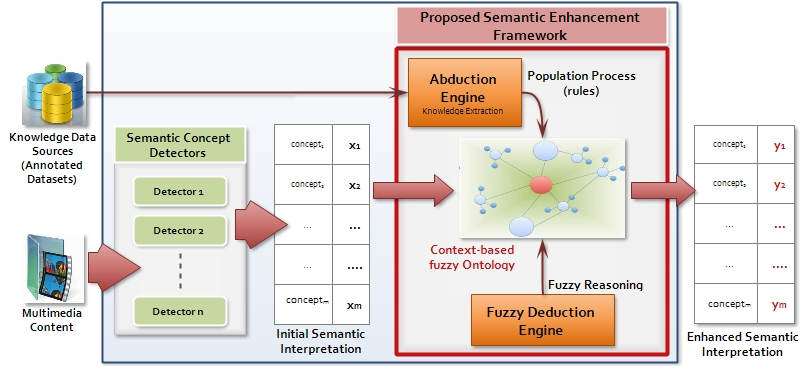
\includegraphics[width=\textwidth]{graphics/systeme}
			\caption{Proposed fuzzy context-based ontology framework for semantic Interpretation}
			\label{fig:system}
		\end{figure}

		
		\subsection{Ontology Structure}
			The objective of our proposed structure for modeling fuzzy knowledge in our ontology 
			is to handle all possible relationships that can exist between semantic concepts 
			within a defined context.

			Classical ontology description languages are not relevant to handle fuzzy knowledge.
			\emph{Fuzzy Description Logics} have been introduced by various approaches to handle 
			uncertainty and vagueness. In our work, we used the $f-\mathcal{SHIN}$ 
			\emph{Description Logics} \citep{Stoilos2005}, 
			and we used the \emph{``tableau''} algorithm \citep{Horrocks2005} for reasoning in
			$f-\mathcal{SHIN}$.  Fuzzy knowledge axioms are grouped in three parts: 
			fuzzy $ABox$ $\mathcal{A}$ for individuals, fuzzy $TBox$ $\mathcal{T}$ for concepts, 
			and fuzzy $RBox$ $\mathcal{R}$ for roles.

			Due to the large amount of multimedia content to handle, it is important to adopt a 
			modular modeling approach. Such ontology modeling has gained widespread attention. 
			Therefore, we propose to define a fuzzy ontology per a defined context.

			Let $\mathcal{K}^{f}$ be a set of fuzzy ontologies defined as follows:
			\begin{equation}
				\begin{array}{ c c l }
					\mathcal{K}^{f} & = &  \{\mathcal{K}^{f}_{t_{1}},\mathcal{K}^{f}_{t_{2}}, 
					\ldots, \mathcal{K}^{f}_{t_{n}}\} \text{ a set of $n$ fuzzy ontologies }  \\
					& &  \text{ where } \mathcal{K}^{f}_{t_{k}} \text{ is a fuzzy ontology for the context } t_{k}.
				\end{array}
			\end{equation}
			
			\begin{definition}
				A fuzzy ontology $\mathcal{K}^{f}_{t_{k}}$ of the context $t_{k}$ can be defined as follows: 

				$\mathcal{K}^{f}_{t_{k}} = \langle \mathcal{T}, \mathcal{R}, \mathcal{A} \rangle$, where
				{
					\begin{equation}
						\begin{array}{ c c l }
							\mathcal{T}  	& = 	& \{\mathsf{Shot} \sqsubseteq \top,\\
							&	& \mathsf{Concept} \sqsubseteq \top,\\
							&	& \mathsf{Context} \sqsubseteq \top,\\
							&	& \mathsf{Context}\sqsubseteq\leq{}1\mathsf{ExistsIn.Shot},\\
							&	& \mathsf{Shot}\sqsubseteq\exists\mathsf{isIndexedBy.Concept},\\
							&	& \mathsf{Concept} \sqsubseteq \exists{}\mathsf{isRelatedTo.Concept}\},\\
							\mathcal{A}	& = 	&
							\{(\langle{}\mathsf{Context},\mathsf{Shot}\rangle:\mathsf{ExistsIn})\geq
							p_{1}\\
							&	& (\langle{}\mathsf{Shot},\mathsf{Concept}\rangle:
							\mathsf{isIndexedBy}) \geq	p_{2}\\
							&	& (\langle{}\mathsf{Concept},\mathsf{Concept}\rangle:\mathsf{isRelatedTo})
							\geq p_{3}\},\\
							\mathcal{R} 	& =	& \{\mathsf{Trans(isRelatedTo)} \\
							&	& \mathsf{Disjoint(isRelatedTo,isRelatedTo^{-})}\}
						\end{array}
					\end{equation}
				}
			\end{definition}
		
		
		$\mathsf{Shot}$, $\mathsf{Context}$ and $\mathsf{Concept}$ are defined as ontology concepts.  
		The $ABox$ $\mathcal{A}$ illustrates possible relationships 
		between concepts, contexts and multimedia content shots defined in the $TBox$ $\mathcal{T}$. 
		Then, $\mathsf{isRelatedTo}$, $\mathsf{isIndexedBy}$ and $\mathsf{ExistsIn}$ 
		are defined as three roles (figure \ref{structure}).
				
		The role $\mathsf{isRelatedTo(Concept, Concept)}$ in the $\mathcal{K}^{f}_{t_{k}}$ ontology
		depicts that there is a generic relationship of a fuzzy weight $p_{3}$ between two concepts 
		within the context $t_{k}$. 
		The \revAnglais{two} roles $\mathsf{ExistsIn(Context, Shot)}$ and
		$\mathsf{isIndexedBy(Shot, Concept)}$ translate a 
		semantic interpretation for a given multimedia content shot. While the role 
		$\mathsf{ExistsIn(Context, Shot)}$ depicts that the context 
		$\mathsf{Context}$ figures in the shot $\mathsf{Shot}$ 
		with a fuzzy weight $p_{1}$, $\mathsf{isIndexedBy(Shot, Concept)}$  role
		depicts that the concept $\mathsf{Concept}$ exists in the shot $\mathsf{Shot}$ 
		with a fuzzy weight $p_{2}$.

		\begin{figure}
			\centering
			 \begin{subfigure}[b]{0.4\textwidth}
      			  	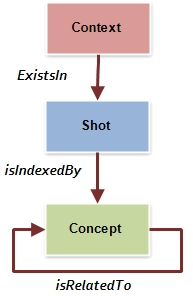
\includegraphics[scale=1]{graphics/structure2}
       				\caption{Conceptual representation of a fuzzy ontology for a given context}
       				\label{structure}
    			\end{subfigure}
			~
			\begin{subfigure}[b]{0.4\textwidth}
      			  	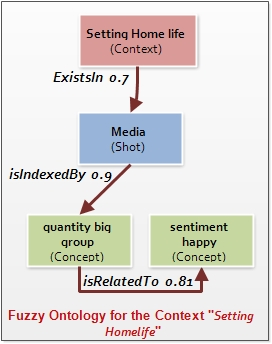
\includegraphics[scale=0.9]{graphics/example}
       				\caption{Example of the $\mathcal{K}^{f}_{Setting~Home~life}$  ontology  
			content for the context \textit{``Setting Home life''}}
       				\label{structure2}
    			\end{subfigure}
			\caption{Conceptual representation and an example of a fuzzy ontology}
		\end{figure}

		For instance, figure \ref{structure2} illustrates the ontology
		structure and individuals for the ontology $\mathcal{K}^{f}_{Setting~Home~life}$
		which is specific for the context $\mathsf{Setting~Home~life}$.
		A shot $\mathsf{Media}$ is indexed by this context with a fuzzy
		degree of $0.7$. Then, the role $\mathsf{isIndexedBy}$ $\mathsf{(Media, Quantity Big Group)}$
		depicts the fact that the shot $\mathsf{Media}$
		is indexed by the concept $\mathsf{Quantity Big Group}$ with a fuzzy
		degree of $0.9$. And finally, 
		the role $\mathsf{isRelatedTo(Quantity Big Group,Sentiment Happy)}$ 
		defines a specific relationship between concepts $\mathsf{Quantity Big Group}$ and 
		$\mathsf{Sentiment Happy}$ with a fuzzy 
		degree of $0.6$ within the ontology $\mathcal{K}^{f}_{Setting~Home~life}$. Thus, if a shot is relevant to the concept 
		$\mathsf{Quantity Big Group}$, it could be relevant too to the concept $\mathsf{Sentiment Happy}$ 
		if the context $\mathsf{Setting~Home~life}$ exists in this shot.

		As described in figure \ref{fig:system}, the proposed framework aims to handle a semantic interpretation 
		as input and to generate an enhanced one as output. Mathematically, and as input, we have a set of shots 
		where each \revAnglais{one} is tagged by some semantic concepts. And as output, the framework \revAnglais{delivers} the same 
		set of images, but with an improved concept tagging. For the ontology side, this set of shots and their 
		related concepts are translated to $Abox$ $\mathcal{A}$ within the fuzzy context-based ontology set. 
		
		\begin{definition}Let $Input$ and $Output$ be sets of quadruplet $(t_{k},c,shot_{i},(\alpha_{1}, \alpha_{2}))$. 
		Each quadruplet depicts that the shot $shot_{i}$ is tagged by the concept $c$ by a fuzzy weight 
		$\alpha_{2}$ within the context $t_{k}$, and tagged by the context $t_{k}$ by a fuzzy weight $\alpha_{1}$.
 		These quadruplets are correlated with the $\mathsf{isIndexedBy}$ and $\mathsf{ExistsIn}$ roles ($\langle(t_{k},s): 
		\mathsf{ExistsIn} \geqslant (\alpha_{1})\rangle$ and $\langle(shot_{i},c) : \mathsf{isIndexedBy} 
		\geqslant (\alpha_{2})\rangle$).
		\end{definition}
		
		\subsection{Abduction Engine and Ontology Population}

			The population process aims to extract new knowledge through an abduction engine and to populate the 
			ontology with new instances defined in a specific context, 
			as well as with their properties and relations. In what follows, we itemize the proposed abduction engine, 
			then we show how to populate the fuzzy context-based ontology with new extracted knowledge.

		\subsubsection{The Abduction Engine}

			In this section, we are particularly interested in the 
			$\mathsf{isRelatedTo}$ role (since the other two roles instances are directly populated 
			from an initial semantic interpretation).

			The key idea behind our method for the abduction engine is to explore similarities 
			between semantic concepts within an annotated multimedia content. Indeed, many annotated 
			multimedia datasets (particularly image and video content) are available and accessible:  
			\emph{ImageCLEF Flickr Photo Annotation and Retrieval} \citep{Thomee2012} and \textsc{TrecVid}  
			\citep{Over2013} training datasets, \emph{Flickr API} and \emph{Picasa API} for image/video 
			crawling, \dots are valuable data sources that can be explored in order to extract knowledge 
			to be inserted into an ontology and to be used then to enhance a semantic interpretation.


			We would like to remind that a \emph{semantic context} is an abstract meaning that cannot be well defined because 
			it makes sense only in particular situations \citep{Elleuch2011, Ksentini2012}. 
			%%%%%%%%%%%%%%%%%%%%%%%%%%%%%%%%%%%%%%%%%%%%%%%%%%%%%%%%%%%%%%%%%%%%%%%%%%%%%%%%%%%%%%
			%%%%%%%%%%%%%%%%%%%%%%%%%%%%%%%%%%%%%%%%%%%%%%%%%%%%%%%%%%%%%%%%%%%%%%%%%%%%%%%%%%%%%%
			%%%%%%%%%%%%%%%%%%%%%%%%%%%%%%%%%%%%%%%%%%%%%%%%%%%%%%%%%%%%%%%%%%%%%%%%%%%%%%%%%%%%%%
			For example, the concept \emph{``airplane\_{}flying''} is considered as
			a context since it specifies a particular relationship between two other
			concepts: \emph{``sky'''} and \emph{``airplane''}. 

			%%%%%%%%%%%%%%%%%%%%%%%%%%%%%%%%%%%%%%%%%%%%%%%%%%%%%%%%%%%%%%%%%%%%%%%%%%%%%%%%%%%%%%
			%%%%%%%%%%%%%%%%%%%%%%%%%%%%%%%%%%%%%%%%%%%%%%%%%%%%%%%%%%%%%%%%%%%%%%%%%%%%%%%%%%%%%%
			%%%%%%%%%%%%%%%%%%%%%%%%%%%%%%%%%%%%%%%%%%%%%%%%%%%%%%%%%%%%%%%%%%%%%%%%%%%%%%%%%%%%%%
			In our case, we define a context as follows:
			\begin{definition} 
				A context is defined as a concept that can stipulate a specific relationship 
				between other concepts.
			\end{definition}

			Thanks to such a definition, we can give a more abstract meaning of a context rather than a \revAnglais{spatial} or 
			temporal information \citep{Brilhault2009}, and also provide an automated way to discover contexts 
			within a concept set.
                	Then, for a given concept $c$, we look for some eventual similarities
			between other concepts within shots annotated with the concept $c$. 
			If such relationships are found, the concept $c$ is considered as a context.

			We use the vector space model based method to compute the similarity between concepts.
			\begin{equation}
				sim(c,d) = cossim(c,d) = \frac{\vec{V_{c}} . 
				\vec{V_{d}}}{|V_{c}| . |V_{d}|}
			\end{equation}
			where for each concept $c$, a weighted vector $V_{c}$ can be constructed as
			\begin{equation}
			V_{c} =\{v^{shot_{1}}_{c},v^{shot_{2}}_{c}, \dots, v^{shot_{m}}_{c}\}
			\end{equation}
			where $v^{shot_{i}}_{c} \in [0,1]$ is the weight of the concept $c$ in the video 
			shot $shot_{i}$, and 
			\begin{equation}
				v_{i}= tf_{shot_{i},c}.idf_{c} = tf_{shot_{i},c}.log\frac{|S|}{|s_{c}|}
			\end{equation}
			where $tf_{shot_{i},c}$ is the frequency of the concept $c$ in the
			video shot $shot_{i}$, $|S|$ is the total number of shots and $|s_{c}|$ is 
			the number of shots tagged by the concept $c$.


			Based on what has just been developed, we propose a formal method to discover contexts. 
			%In our case, we populate a fuzzy ontology $\mathcal{K}^{f}_{t_{k}}$ of the context $t_{k}$ as follows:
			%%%%%%%%%%%%%%%%%%%%%%%%%%%%%%%%%%%%%%%%%%%%%%%%%%%%%%%%%%%%%%%%%%%%%%%%%%%%%%%%%%%%%%
			%%%%%%%%%%%%%%%%%%%%%%%%%%%%%%%%%%%%%%%%%%%%%%%%%%%%%%%%%%%%%%%%%%%%%%%%%%%%%%%%%%%%%%
			%%%%%%%%%%%%%%%%%%%%%%%%%%%%%%%%%%%%%%%%%%%%%%%%%%%%%%%%%%%%%%%%%%%%%%%%%%%%%%%%%%%%%%			
			Thus, we define the similarity $sim_{t_{k}}(c, d)$ as a similarity measurement between the 
			two concepts 
			$c$ and $d$ within the context $t_{k}$. This similarity will be used as a fuzzy degree 
			for the rule that relates the concepts $c$ to the concept $d$ within the role 
			$\mathsf{isRelatedTo}$ for the $\mathcal{K}^{f}_{t_{k}}$ ontology.


			Furthermore, $\mathsf{isRelatedTo}$ is a \revAnglais{non-symmetric}  role
			(as appears in the \emph{Rbox} $\mathcal{R}$). 
			As an example, when talking about the concept \emph{``car\_racing''}, 
			it is obvious that we talk about the concept \emph{``car''}, but  the \revAnglais{opposite}
			in not often true. Thus $sim(car,car\_racing) \neq sim(car\_racing ,car)$.
			To do that, the similarity function that is used to compute the similarity $sim_{t_{k}}(c, d)$ 
			in a defined context  $t_{k}$ has to be \revAnglais{non-symmetric}. 
			Then, the two vectors $V_{c}$ and $V_{d}$ are modified as follow to ensure that  
			$sim_{t_{k}}(c, d) \neq sim_{t_{k}}(d, c)$:

		
		\begin{equation}
			\begin{array}{ c c l }
			V_{c} & = & \{v^{shot_{1}}_{c},v^{shot_{2}}_{c}, \dots, v^{shot_{m}}_{c}\}\\
			%%%%%%%%%%%%%%%%%%%%%%%%%%%%%%%%%%%%%%%%%%%%%%%%%%%%%%%%%%%%%%%%%%%%%%%%%%%%%%%%%%%%%%
			%%%%%%%%%%%%%%%%%%%%%%%%%%%%%%%%%%%%%%%%%%%%%%%%%%%%%%%%%%%%%%%%%%%%%%%%%%%%%%%%%%%%%%
			%%%%%%%%%%%%%%%%%%%%%%%%%%%%%%%%%%%%%%%%%%%%%%%%%%%%%%%%%%%%%%%%%%%%%%%%%%%%%%%%%%%%%%			
			%V_{d} & = & 
			V_{d} & = & 
			%%%%%%%%%%%%%%%%%%%%%%%%%%%%%%%%%%%%%%%%%%%%%%%%%%%%%%%%%%%%%%%%%%%%%%%%%%%%%%%%%%%%%%
			%%%%%%%%%%%%%%%%%%%%%%%%%%%%%%%%%%%%%%%%%%%%%%%%%%%%%%%%%%%%%%%%%%%%%%%%%%%%%%%%%%%%%%
			%%%%%%%%%%%%%%%%%%%%%%%%%%%%%%%%%%%%%%%%%%%%%%%%%%%%%%%%%%%%%%%%%%%%%%%%%%%%%%%%%%%%%%			
			\{v^{shot_{1}}_{d},v^{shot_{2}}_{d}, \dots, v^{shot_{m}}_{d}\}\\
			& & \text{ where for every considered shot } shot_{i} \text{ in both } V_{c} \text{ and } V_{d},\\
			& &  \text{we have } v^{shot_{i}}_{c}\neq 0 \text{ and } v^{shot_{i}}_{t_{k}} \geqslant \gamma
			\end{array}
		\end{equation}
		
		we suggest $\gamma \in [0,1]$  as a threshold to judge if a concept is strongly relevant 
		to a video shot or not. Thus, only tagged shots by the concept $c$ and that are strongly 
		tagged by the concept/context $t_{k}$ are considered for both $V_{c}$ and $V_{d}$ in order to guarantee 
		the \revAnglais{non-symmetric} aspect of the role $\mathsf{isRelatedTo}$.


		\subsubsection{Ontology Population}	
		\label{pop1}
		The ontology population  passes through two steps: 
		\begin{enumerate}
			\item \textit{\revAnglais{Knowledge} Population}: For each defined context $t_{k}$, 
			this step constructs an empty ontology $\mathcal{K}^{f}_{t_{k}}$ based on the proposed structure detailed in 
			the previous section. Then, the context $t_{k}$ is instantiated as an individual
			from the class $\mathsf{Context}$. Next, for every new similarity 
			$sim_{t_{k}}(c, d)$ computed between two concepts $c$ and $d$ within the 
			context $t_{k}$, two new instantiations from the class $\mathsf{Concept}$ 
			are introduced in the ontology for both concepts $c$ and $d$, and finally  
			a new $\mathsf{isRelatedTo}$ role instantiation between $c$ and $d$  
			is inserted to the $\mathcal{K}^{f}_{t_{k}}$ ontology with a fuzzy weight
			equal to this similarity value.
 
			\item \textit{Semantic Interpretation Population}
			In this step, semantic interpretations about shots 
			are introduced to the set of fuzzy ontologies $\mathcal{K}^{f}$. 
			For a given shot $shot_{i}$, and for each context $t_{k}$, if $shot_{i}$ 
			is tagged by the context $t_{k}$, then:
				\begin{enumerate}
					\item the shot $shot_{i}$ is instantiated as an individual from 
					the class $\mathsf{Shot}$,
					\item a new instantiation of the role $\mathsf{ExistsIn}$ is introduced 
					between $shot_{i}$ and $t_{k}$ within the ontology $\mathcal{K}^{f}_{t_{k}}$,
					\item for every concept $c$ that tags $shot_{i}$, $c$ is introduced to the 
					ontology $\mathcal{K}^{f}_{t_{k}}$ as an individual from the class 
					$\mathsf{Concept}$, and a new $\mathsf{IsIndexedBy}$ role \revAnglais{instantiation}
					is created between $shot_{i}$ and $c$.
				\end{enumerate}
		\end{enumerate}

		Once the two steps are performed, a set of fuzzy context-based ontology \revAnglais{is} built and 
		ready to fire the reasoning engine (the deduction engine) in order to
		generate an enhanced semantic interpretation.
		
		\subsection{Ontology Reasoning}
		Within the scope of reasoning in this paper, we are particularly interested in the outputs that
		such a system produces. In such a case, and for each ontology $\mathcal{K}^{f}_{t_{k}}$ 
		of the context $t_{k}$, we generate 
		the corresponding ontology $\mathcal{K'}^{f}_{t_{k}}$ as an ontology that handle enhanced 
		semantic interpretations. This is done by 
		interpreting the $Abox$ $\mathcal{A}$ in order to look for updated or additional relationships between 
		$\mathsf{Shot}$ and $\mathsf{Concept}$ (for the role name
		$\mathsf{isIndexedBy}$).

		We used and adapted the \emph{``tableau''} based reasoning algorithm \citep{Dentler2011}. The latter  
		adopts a federated reasoning process with our set of fuzzy ontologies. Thus, each fuzzy ontology is 
		associated with a local reasoner. The final and global reasoning  result is inferred through 
		all the local reasoner results. 


		Considering concepts and roles as fuzzy sets, the semantics of concepts and roles are defined 
		by fuzzy interpretations $\mathcal{I} = \langle{}\triangle^{\mathcal{I}}= , \cdot^{\mathcal{I}}\rangle{}$, 
		where $\triangle^{\mathcal{I}}$ is a nonempty domain, and $\cdot^{\mathcal{I}}$ is an interpretation 
		function mapping individuals $a$ into $a^{\mathcal{I}} \in \triangle^{\mathcal{I}}$,
		and mapping concept (roles) names $A(R)$ into membership functions 
		$A^{\mathcal{I}}(R^{\mathcal{I}}) : \triangle^{\mathcal{I}} (\triangle^{\mathcal{I}} * \triangle^{\mathcal{I}} ) 
		\rightarrow [0, 1]$. 
		An interpretation $\mathcal{I}$ satisfies a knowledge database $\mathcal{K}^{f}_{}$, 
		if and only if  $\mathcal{I}$ satisfies any
		axiom in $\mathcal{R}$, $\mathcal{T}$ and $\mathcal{A}$. $\mathcal{K}^{f}_{}$ is satisfiable 
		if and only if it has a fuzzy model.

		We define the symbols  $\rhd$ and  $\lhd$ as a placeholder for the  inequalities 
		($\leq$, $<$, $\geq$ and $>$) and the symbol $\bowtie$ as a placeholder for all types of inequalities.
		
		\begin{definition}
			let $R_{A}$ be the set of roles occurring in $\mathcal{A}$, $I_{\mathcal{A}}$ the set 
			of individuals in $\mathcal{A}$ and $\mathcal{X} = \{\leq, <, \geq, >\}$. A fuzzy tableau 
			$T$ for $\mathcal{A} ~ w.r.t ~ \mathcal{R}$ is a quadruple
			$(S, \mathcal{L, E, V})$ in such a way that:
			\begin{itemize}
				\item $S$ is a nonempty set of individuals (considered also as nodes),
				\item $\mathcal{L} : S \longrightarrow 2^{sub(A)} \times \mathcal{X} \times [0,1]$ 
					maps each individual in $S$ to membership triples,
				\item $\mathcal{E} : R_{A} \longrightarrow 2^{S \times S} \times \mathcal{X} \times [0,1]$ 
					maps each role to membership triples,
				\item $\mathcal{V} : I_{\mathcal{A}} \longrightarrow S$ maps individuals occurring in 
					$\mathcal{A}$ to elements in $S$.
			\end{itemize}
		For all	$s,t \in S$, $R\in R_ {A}$ and $C,E \in sub(\mathcal{A})$, $T$ satisfies a particular 
		transformation rule defined in algorithm \ref{algo1}	
		(in addition to default transformation rules defined in \citep{Stoilos2005}).	

		\begin{algorithm}
				\If	{ $\langle(t_{k},shot_{i}) : \mathsf{ExistsIn} \bowtie \alpha_{1}\rangle 
					\in \mathcal{A}$ AND \\
					$\langle(shot_{i},c) : \mathsf{isIndexedBy} \bowtie \alpha_{2}\rangle \in \mathcal{A}$ 
					AND \\
					$\langle(c,d) : \mathsf{isRelatedTo} \bowtie \alpha_{3}\rangle \in \mathcal{A}$}
					{
					 \lIf	{$\langle(shot_{i},d) : \mathsf{isIndexedBy} \bowtie 
						\alpha_{4}\rangle \notin \mathcal{A}$} 
						{\\$\mathcal{A'} := \mathcal{A} \sqcup \{ \langle{}\mathsf{shot_{i}},
							\mathsf{d}\rangle:
							\mathsf{isIndexedBy}) \bowtie \alpha_{4}\}$\\
							and $\langle \langle\mathcal{V}(shot_{i}),\mathcal{V}(d)\rangle
							\bowtie \alpha_{4}\rangle 
							\in \mathcal{E}(\mathsf{isIndexedBy})$ \\
							where $\alpha_{4} = \alpha_{1} \times \alpha_{2} \times \alpha_{3}$}
						\lElse{$\langle \langle\mathcal{V}(shot_{i}),\mathcal{V}(d)\rangle
							\bowtie \alpha_{4}'\rangle 
							\in \mathcal{E}(\mathsf{isIndexedBy})$ \\
							where $\alpha_{4}' = max(\alpha_{4}, (\alpha_{1} \times \alpha_{2}
							\times \alpha_{3}))$}}
					\caption{Transformation Rule: Property 1}
					\label{algo1}
				\end{algorithm}
				
		\end{definition}
		Property 1 is a consequence of the fact that if there are three \revAnglais{axioms} in $\mathcal{A}$ 
		where $shot_{i}$ is indexed by a concept $c$, and the context $t_{k}$ exists in the $shot_{i}$, 
		then the $shot_{i}$ could be indexed by the concept $d$ taking into account that within the 
		fuzzy ontology of the context $t_{k}$, there is a relationship between the two concepts $c$ and $d$.
		If this new deduced relationship already exists in the ontology, then we only update its fuzzy weight.

		We used and adapted a \emph{“tableau”} based reasoning algorithm.
 		For a given context-based ontology, the latter model the knowledge in form of 
		a tree in which nodes correspond to individuals (semantic concepts, semantic contexts and shots) 
 		and edges correspond to the defined roles ($\mathsf{isIndexedBy}$,$\mathsf{isRelatedTo}$,
 		and $\mathsf{ExistsIn}$).
 		Each node $x$ is labeled with a set of concepts $\mathsf{L}(x)$ that the
 		individual must satisfy, and each edge is labeled with a role name.
 		The reasoning algorithm starts with a single node labeled $\{D\}$ (in our case, a
 		node labeled as a shot), and proceeds by repeatedly applying a set of expansion 
		rules that recursively decompose the concepts in node labels.

		The reasoning process should not be endless. This problem can \revAnglais{deal} with the use 
		of a blocking technique: stopping the expansion when a cycle is detected. The 
		blocking procedure consists in checking the label of each new node $y$, and if 
		it's a subset of the label of an existing node $x$, then the expansion of $y$ 
		is stopped: $x$ is said to block $y$.
		
		Thus, the reasoning process termination is \revAnglais{guaranteed}: all concepts in node labels
		are derived from the decomposition of $D$, so all node labels must be a subset  
		of the sub-concepts of $D$. A cycle should be avoided within a finite number of expansion steps.

		%%%%%%%%%%%%%%%%%%%%%%%%%%%%%%%%%%%%%%%%%%%%%%%%%%%%%%%%%%%%%%%%%%%%%%%%%%%%%%%%%%%%%%%%%%%%%%%%%%
		%%%%%%%%%%%%%%%%%%%%%%%%%%%%%%%%%%%%%%%%%%%%%%%%%%%%%%%%%%%%%%%%%%%%%%%%%%%%%%%%%%%%%%%%%%%%%%%%%%
		\begin{algorithm}
			
			\SetAlgoLined
			%\KwData{$Input \neq \emptyset$ and $Output = \emptyset$ }
			%\KwResult{$Output \neq \emptyset$ }
			\For{each shot \textbf{$shot_{i} \in \mathsf{Shot}$}}{
				\For{each concept \textbf{$c$} connected with the shot 
				\textbf{$shot_{i}$} by an $\mathsf{isIndexedBy}$ labeled edge}{
					Handle\_isRelatedTo\_Role($shot_{i}$,$c$);
				}
			}
			\caption{Reasoning Process for enhancing a semantic interpretation about shots.}
			\label{algo112}
		\end{algorithm}
		
		%%%%%%%%%%%%%%%%%%%%%%%%%%%%%%%%%%%%%%%%%%%%%%%%%%%%%%%%%%%%%%%%%%%%%%%%%%%%%%%%%%%%%%%%%%%%%%%%%%
		%%%%%%%%%%%%%%%%%%%%%%%%%%%%%%%%%%%%%%%%%%%%%%%%%%%%%%%%%%%%%%%%%%%%%%%%%%%%%%%%%%%%%%%%%%%%%%%%%%
		
		\begin{algorithm}
			
			\SetAlgoLined
			%\KwData{$Input \neq \emptyset$ and $Output = \emptyset$ }
			%\KwResult{$Output \neq \emptyset$ }
			\textbf{Function} Handle\_isRelatedTo\_Role($shot_{i}$,$c$)\\
			  \eIf{isMarked($c$)}{
			  return\;}
			  {
			  		\For{each concept $d$ connected with $c$ by an edge labeled
			  		$\mathsf{isRelatedTo}$}{Mark($c$)\;
					apply Algorithm \ref{algo1} \;
					Handle\_isRelatedTo\_Role($shot_{i}$,$d$)\;
				}	
			}
			\caption{Recursive call for \emph{``Handle\_isRelatedTo\_Role()''} Function}
			\label{algo111}
		\end{algorithm}
		%%%%%%%%%%%%%%%%%%%%%%%%%%%%%%%%%%%%%%%%%%%%%%%%%%%%%%%%%%%%%%%%%%%%%%%%%%%%%%%%%%%%%%%%%%%%%%%%%%
		%%%%%%%%%%%%%%%%%%%%%%%%%%%%%%%%%%%%%%%%%%%%%%%%%%%%%%%%%%%%%%%%%%%%%%%%%%%%%%%%%%%%%%%%%%%%%%%%%%

		The $\mathsf{isRelatedTo}$ role is cyclic and transitive. Such a
		definition \revAnglais{makes} the termination and the decidability of our reasoning process hard. We adapted 
		the \emph{``tableau''} algorithm is such a way to  solve this problem. 
		Apart from the generic blocking technique above detailed, we used a second 
		blocking technique which marks every passage through  
		semantic concepts that are connected with $\mathsf{isRelatedTo}$ role labeled
		edges. We used two functions: $Mark(c)$ which marks a concept $c$, and
 		$isMark(c)$ which returns whether the concept $c$ is marked or not yet.

		Algorithms \ref{algo112} and \ref{algo111} detail how we extend a semantic interpretation of a given
 		shot taking into consideration the proposed blocking technique. 

		The node marking test in the algorithm \ref{algo111} allows to detect an
 		eventual cycle. Then, a possible endless call to the
 		\emph{``Handle\_isRelatedTo\_Role()''} recursive function is blocked. 
		The proposed algorithm achieved the decidability of our reasoning process.

		\subsection{Ontology Evolving}
		\label{section:evolving}
		Evolving and updating fuzzy knowledge is a task that must be addressed in an ontology life cycle. 
		Such a test consists in updating the ontology content in order to take into account both, eventual erroneous 
		or senseless knowledge, or newer knowledge. In our work, we consider the evolution of ontology individuals content 
		and not the conceptual level. Then, only individuals and \revAnglais{inter-relationships} in $Abox$ $\mathcal{A}$ 
		could be updated.

		The evolving task proceeds as follows: Let $\mathcal{A}$ be the $ABox$ of an ontology, and $\mathcal{A_{+}}$ 
		the updated one. %, and $\mathcal{A'}$ the final considered knowledge after the evolving process.
 		Then the evolving task can be illustrated with the algorithm \ref{algo3}. The latter always \revAnglais{considers}
		the new discovered knowledge by updating the fuzzy weight of a $\mathsf{isRelatedTo}$ 
		role to the new value defined in $\mathcal{A_{+}}$.
		
		\begin{algorithm}
				
				\If	{$\langle(c,d) : \mathsf{isRelatedTo} \bowtie \alpha \rangle \in \mathcal{A}$ AND \\
					 $\langle(c,d) : \mathsf{isRelatedTo} \bowtie \alpha'\rangle \in \mathcal{A_{+}}$ }
					{
					 $\mathcal{A} := \mathcal{A}  \diagdown \{
					 \langle{}(\mathsf{c},\mathsf{d}):
							\mathsf{isRelatedTo}\rangle{} \bowtie \alpha\}$\\
					$\mathcal{A} := \mathcal{A} \sqcup \{ \langle{}(\mathsf{c},\mathsf{d}):
							\mathsf{isRelatedTo}\rangle{} \bowtie \alpha'\}$\\
					}
				\caption{The knowledge evolving task}
				\label{algo3}
		\end{algorithm}

		In what follows, we show how to generate the new $ABox$ $\mathcal{A_{+}}$ used to update the ontology content. 
		Thus, we consider that the defined fuzzy ontologies are populated through
		a knowledge discovery technique based 
		on annotation data. We consider, too, that this extracted knowledge may
 		be inaccurate depending on many factors (annotators quality, dataset content quality, \dots). 
		Then, we propose  to correct the ontology contents 
		through inspecting $\mathsf{isRelatedTo}$ roles by human experts. 

		We thus propose a user interface to let the experts give their relevance judgment for a given role within a given 			contextual ontology. For a given context $t_{k}$ and an affiliated $\{ \langle{}(\mathsf{c},\mathsf{d}): 
		\mathsf{isRelatedTo}\rangle{} \bowtie \alpha\}$ role, this user interface shows
 		to the expert a set of rows where each one details one shot that both the context 
		$t_{k}$ and the concept $c$ exist. The expert then has to select one from these four options:
		\begin{itemize}
			\item $Strongly~Relevant$ when the concept $d$ effectively in the showed shot. We 
				consider that the fuzzy weight for this case is higher or equal to $0.7$,
			\item $Weakly~Relevant$ When the concept $d$ may \revAnglais{exist} in the showed shot. We 
				consider that the fuzzy weight for this case is higher or equal to $0.3$ 
				and lower than $0.7$,
			\item $Not~Relevant$ When the concept $d$ does not exist in the showed shot. We 
				consider that the fuzzy weight for this case is lower than $0.3$,
			\item $Skip$ when the expert \revAnglais{cannot} judge clearly if the concept $d$ 
				exists or not in the showed shot.
		\end{itemize} 
		
		The original value of a fuzzy weight of a given role is taken into
		consideration and appears when the evolving user interface displays a role to 
		an expert. In fact, every role is displayed 
		with its fuzzy weight, and the expert \revAnglais{judges} to input his judgment (if he
		\revAnglais{finds} that the role is not pertinent) or to skip to analyze another role.
		
		After the evaluation process done by the experts, the \revAnglais{knowledge} evolving task computes new fuzzy 
		weights for evaluated roles. These weights are computed as follows:
		Let $N_{experts}$ be the number of experts who evaluated the role $r$. Let $N_{StrongR}$, 
		$N_{WeakR}$ and $N_{NotR}$ be, respectively, the number of $Strongly~Relevant$, $Weakly~Relevant$ 
		and $Not~Relevant$ judgments made by the $N_{experts}$ experts for the role $r$ where:
		\begin{equation}
			N_{experts} \geqslant  N_{StrongR} +  N_{WeakR} +  N_{NotR}.
		\end{equation}

		Then, we compute the new fuzzy weight for the evaluated role $r$ as follows:
		
		\begin{equation}
		\alpha'=\left\{
			\begin{array}{l c}
				max(\alpha, \frac{N_{StrongR}}{N_{experts}})	& 
					\text{\scriptsize{if $N_{StrongR} \geqslant (N_{WeakR},N_{NotR})$}} \\
				min(\alpha, \frac{1-N_{WeakR}}{N_{experts}}) & 
					\text{\scriptsize{if $N_{WeakR} > (N_{StrongR},N_{NotR})$}}\\
				min(\alpha, \frac{1-N_{NotR}}{N_{experts}})  &
					\text{\scriptsize{if $N_{NotR} > (N_{StrongR},N_{WeakR})$}}
			\end{array}
		  \right.
		\end{equation}

		The equation above is inspired by the majority vote. The new computed role 
		fuzzy weight is based on whether experts are commonly improving or disregarding a role.
		
		For an analyzed role, only one new fuzzy weight will be considered
		and introduced to the ontology. Thus, no eventual conflicting situation 
		occurs when firing the reasoning engine.
		This choice is preselected by the initial value of fuzzy role weight.

		\subsection{Approach Scalability}

		The scalability aspect is very important and concerns mainly two aspects: 
		how our framework \revAnglais{performs} when a large amount of concepts 
		and interrelationships are defined, and when the number of contexts increases. 

		Our proposed approach could be considered as scalable:
		at first, the $Tbox$ $\mathcal{T}$ remains unchanged, and only new $Abox$ $\mathcal{A}$ 
		instances are \revAnglais{being} handled within the defined contextual ontologies. Then, the amount of knowledge 
		populated within an ontology depends only on what has been gathered from annotated 
		video datasets in addition to the semantic interpretation of the analyzed video shot. 
		Secondly, since the proposed approach is decomposed into several ontologies, 
		the deduction engine is applied only on $Abox$ $\mathcal{A}$ that are related only to each defined contexts. 
		This leads to an optimized and a lightened reasoning process: only partial 
		defined roles in ontologies will be considered and fired.
		
		In the next section, we conduct an experiment to investigate our approach effectiveness and scalability.
		

		
	%%%%%%%%%%%%%%%%%%%%%%%%%%%%%%%%%%%%%%%%%%%%%%%%%%%%%%%%%%%%%%%%%%%%%%%%%%%%%%%%%%%%%%%%%%
	%%%%%%% EVALUATION
	\section{Experimental Study}
		\label{c2_3}
		In the previous chapter, we discussed our participation within \revAnglais{the} \textsc{TrecVid 2010}. 
		Only the deduction process was taken into consideration since we used a manually predefined 
		set of rules, and  we were interested in visual (key frames) semantic analysis. 
		
		In order to illustrate the semantic enhancement of concept detection introduced 
		by our proposed ontology-based framework, we have conducted an experiment within a 
		different multimedia evaluation campaign. Hence, we expose the experimental setup and the 
		obtained results of our framework within \textit{ImageClef 2012} \citep{Thomee2012}
		at the \textit{Photo Annotation and Retrieval} Task. 
		Finally, we discuss the scalability of our proposed framework.


		\subsection{Datasets Description}

		The \textit{ImageClef 2012} Photo Annotation and Retrieval task provides a dataset built from
		Flickr social shared photos. This image dataset consists of 25 thousand images:
		15 thousand for the learning process and 10 thousand for the test one. In addition
		to the images, 94 semantic concepts are defined referring to many and various 
		subjects (people, nature, events, \dots). 

		\subsection{Evaluation metrics}
		In order to be able to compare different indexing approaches, various system 
		effectiveness metrics have been used. These metrics are commonly based on precision
		(which is defined as the number of relevant answers as a part of the total number
		of retrieved ones), and recall (which is defined as the number of relevant answers
		as part of total relevant ones in the collection). In our experiments, we consider the two
 		evaluation measures: \emph{Interpolated Mean Average Precision} (\textit{$map_{i}$}) and \emph{Interpolated 
		Geometric Mean Average Precision} (\textit{$gmap_{i}$}) \citep{Thomee2012}
		for \revAnglais{the} \textit{ImageClef 2012} Flickr Photo Annotation and Retrieval task.

		The \textit{$gmap_{i}$} is considered as an extension to the \textit{$map_{i}$} measure as it uses the same 
		computing procedure, but it's very useful when focusing on low performing semantic 
		interpretation for particular concepts

		
			\subsection{Experiments with \textit{ImageClef 2012} dataset}
		
		With this experiment, we aim to explore all the 15 thousand annotated images in order 
		to extract valuable fuzzy \revAnglais{Knowledge}. The latter will be used then within the deduction engine 
		to evaluate the knowledge-based semantic enhancement performances. The obtained results will be compared 
		to a \revAnglais{non-knowledge-based} concept detection approach detailed in \citep{Ksibi2012}. Thus, we
		used the results given by the \revAnglais{non-knowledge-based} method as input for our framework looking 
		for enhancing the semantic interpretation and for proving the effectiveness of the use of
		fuzzy context-based ontology and fuzzy reasoning in multimedia retrieval
		systems.

			\subsubsection{The abduction process}
		In the interest of populating our proposed ontology, we start by defining the set of considered contexts. 
		At first, we consider every concept as a context, and then, we look for specific relationships between other 
		concepts within this context. If any relationships are found, the defined concept will be considered
		as a context, else, the concept will not be considered as a context.
		By doing so, our proposed framework can provide automatically a set of context to work with. We consider 
		that a context exists in a shot only if this latter is strongly tagged by that context to a degree equal 
		to or higher than $0.7$. Then, we adjust the value of the threshold $\gamma$ at $0.7$.

		Our experimentation has led to define 90 contexts among the defined 94 concepts in \textit{ImageClef 2012} dataset. 
		Table \ref{table:context-based_ontology} enumerates a partial view of this set of contexts, 
		and shows the first and the last 5 contexts sorted 
		by the number of extracted $\mathsf{isRelatedTo}$ roles.
		%with a fuzzy weight equal to or higher than $0.5$.
		\begin{table*}
			\centering	
			\caption{Distribution of extracted $\mathsf{isRelatedTo}$ roles according to 
			their fuzzy weights and the defined context}
			\label{table:context-based_ontology}
				\begin{tabular}{c l c c c c c c c c c c} \hline
				~&\multirow{3}{*}{\textbf{Detected Contexts}}& \multicolumn{4}{c}{\scriptsize 
						\textbf{Number of extracted fuzzy rules according}}\\
				~& & \multicolumn{4}{c}{\scriptsize  \textbf{to their fuzzy weight intervals}}\\ 		
				~& & \small{$[0, 0.3[$} & \small{$[0.3, 0.5[$} & \small{$[0.5, 0.7[$} & 
				\small{$[0.7, 1.0]$} \\ 		\hline \hline
			\scriptsize{1}&\small{sentiment\_euphoric}	&783	&605	&510	&534\\
			\scriptsize{2}&\small{sentiment\_happy}		&2020	&864	&519	&444\\
			\scriptsize{3}&\small{setting\_sportsrecreation}&1264	&752	&483	&456\\ 
			\scriptsize{4}&\small{age\_child}		&1045	&649	&493	&441\\ 
			\scriptsize{5}&\small{relation\_familyfriends}	&1150	&903	&398	&522\\ \hline
			\scriptsize{86}&\small{fauna\_cat}		&115	&105	&91	&203\\ 
			\scriptsize{87}&\small{fauna\_insect}		&107	&63	&43	&192\\
			\scriptsize{88}&\small{fauna\_rodent}		&43	&53	&43	&139\\ 
			\scriptsize{89}&\small{fauna\_amphibianreptile}	&24	&29	&43	&127\\ 
			\scriptsize{90}&\small{fauna\_spider}		&3	&20	&16	&48\\ \hline \hline
			\multicolumn{2}{c}{\textbf{All contexts}}	&91803 	&50210	&27435	&33667\\
			 \hline \hline
			\multicolumn{2}{c}{\textbf{Total}}& \multicolumn{4}{c}{\textbf{203115 $\mathsf{isRelatedTo}$ 
								roles}}\\ \hline
			\end{tabular}
		\end{table*}
		

		Taking some roles as examples, we focus on the contexts \emph{age\_adult}, \emph{transport\_car},
		\emph{setting\_homelife} and \emph{age\_teenager}:
		\begin{equation*}
			\begin{array}{ c c l l}
			R1 & - &\mathsf{isRelatedTo}_{age\_adult} 
				& (age\_teenager,sentiment\_scary) \geq 0.12\\
			R2 & - &\mathsf{isRelatedTo}_{transport\_car}
				& (sentiment\_happy,timeofday\_day) \geq 0.95\\
			R3 & - &\mathsf{isRelatedTo}_{setting\_homelife} 
				& (quantity\_biggroup,sentiment\_happy) \geq 0.81\\
			R4 & - &\mathsf{isRelatedTo}_{age\_teenager}
				& (sentiment\_funny,quantity\_two) \geq 0.48
			
			\end{array}
		\end{equation*}

		The role $R1$ depicts that in the case of a shot tagged by the concept \emph{age\_teenager} 
		and strongly tagged by the concept \emph{age\_adult} (here considered as a context), then the concept 
		\emph{sentiment\_scary} could exist in the same shot. Naturally, this case is not always true, 
		and this is why the fuzzy weight of this role is very weak ($0.12$).
		Then, the roles $R2$  and $R3$ depict strong relationships between the two concepts 
		\emph{sentiment\_happy} and \emph{timeofday\_day} within the context \emph{transport\_car},
		and between the two concepts \emph{quantity\_ biggroup} and \emph{sentiment\_happy} within 
		the context \emph{setting\_homelife}. These two relationships are considered as strong roles 
		(where the fuzzy weights are high).

		Finally, and after extracting knowledge from the learning dataset and generating $\mathsf{isRelatedTo}$
		roles, these roles are introduced into the corresponding fuzzy context based ontology (as detailed in section \ref{pop1}).
		
		We continue to experiment deduction engine as a fuzzy reasoning process based 
		on these roles to assess the semantic enrichment in the next section.

		\subsection{Enhancement Evaluation}
		To evaluate our proposed framework, we have compared our results with an image annotation 
		method detailed in \citep{Ksibi2012} within the \emph{Flickr Photo Annotation Task}. 
		The latter is based on constructing a semantic context network to depict intrinsic 
		contextual information between concepts in order to enhance automatic photo annotation performances.
		In our work, we are interested in improving this method. Thus, we used the results given by this 
		method as input to our framework aiming at enhancing the semantic interpretation.


		Considering constructed fuzzy context-based ontology set in the previous section, 
		we introduce the $Input$ set  to these ontologies. Then, the deduction engine is fired. 
		Finally, the $Output$ set is extracted and translated into a semantic interpretation as an 
		enhanced one. For the deduction engine, only 
		$\mathsf{isRelatedTo}$ roles with a fuzzy weight higher or equal to $0,7$ are addressed. 
		We think that the other roles figure weak fuzzy weights and shouldn't be used in the deduction process.
		
		After extracting the $Output$ set, the system is ready for evaluation. So, we used 
		the evaluation tool supplied by \emph{ImageCLEF} 
		(\emph{imageclef2012CR}). We carried out unit evaluations over ontologies 
		(each ontology is evaluated separately). Finally, we applied an overall assessment showing 
		the performance of our framework (all ontologies combined). 

		Table \ref{overall} displays enhancement performances delivered by our proposed framework over 
		the \revAnglais{non-knowledge-based} approach detailed in \citep{Ksibi2012}. Table \ref{unit} shows enhancement 
		performances delivered by each defined fuzzy context-based ontology.
				

		In order to make table \ref{overall} and table \ref{unit} interpretation easier, three styles 
		were used: bold values depict enhancing performances compared to the corresponding 
		evaluation of the system detailed in \citep{Ksibi2012}, underlined values depict a 
		decreasing performance, and finally, the \revAnglais{non-styled} values depict same performance 
		as reference. 

		\begin{table*}[ht!]
			\centering	
			\caption{\textsc{ImageClef 2012}: Overall performance evaluation}
			\label{overall}
		\begin{tabular}{p{6cm}|c|c|c|c} 
			&
			\multicolumn{2}{c|}{\textbf{\textit{map$_{i}$}}} &
			\multicolumn{2}{c}{\textbf{\textit{gmap$_{i}$}}}  \\
			& \textit{Value} & \textit{Enhancement} & \textit{Value} & \textit{Enhancement}  \\
			\hline  
			Our proposed framework  & 
						\textbf{0,1324} & $5.08 \% $ & 
						\textbf{0, 0807} & $3.46 \% $ \\
			System in \cite{Ksibi2012}   & $0.126$ & - & $0.078$  \\
			\hline 
		\end{tabular}
		\end{table*}


\begin{table*}[ht!]
	\centering
	\caption{\textsc{ImageClef 2012}: Unit performances evaluation}
	\label{unit}
\begin{scriptsize}
\begin{tabular}{|c|lcc||c|lcc|}
	\hline
	\#  &\textbf{\textit{Context}}	& \multicolumn{2}{l||}{\textbf{\textit{{~~~~Evaluation} }}}
	&
	\# 		& 
	\textbf{\textit{Context}} 	& 
	\multicolumn{2}{l|}{\textbf{\textit{{~~~~Evaluation} }}} \\
	%\hline
	%#
        	&  &  \textbf{map$_{i}$} &  \textbf{gmap$_{i}$} &   & & \textbf{map$_{i}$}	&  \textbf{gmap$_{i}$}     \\
	\hline \hline

1&age\_adult&		0.126&		0.078&			46&scape\_forestpark&	\textbf{0.1277}& 	\textbf{0.0792}\\
2&age\_baby&		\textbf{0.1275}&\textbf{0.0787}&	47&scape\_graffiti&	\textbf{0.1265}&	\textbf{0.0784}\\    
3&age\_child&		0.126&		0.078&			48&scape\_mountainhill&	\textbf{0.1294}&	\textbf{0.0801}\\         
4&age\_elderly&		0.126&		0.078&			49&scape\_rural&	\textbf{0.1279}&	\textbf{0.0792}\\  
5&age\_teenager&	\textbf{0.1279}&\textbf{0.0793}&	50&sentiment\_active&   \textbf{0.1284}&	\textbf{0.079}\\         
6&celestial\_moon&	\textbf{0.1273}&\textbf{0.0787}&	51&sentiment\_calm&	\textbf{0.1261}&    	\textbf{0.0781}\\         
7&celestial\_stars&	\textbf{0.1277}&\textbf{0.0789}&	52&sentiment\_euphoric&	\textbf{0.1281}&	\textbf{0.0794}\\         
8&celestial\_sun&	\textbf{0.1269}&\textbf{0.0786}&	53&sentiment\_funny&	\textbf{0.1272}&	\textbf{0.0788}\\         
9&combustion\_fireworks&\textbf{0.1268}&\textbf{0.0785}&        54&sentiment\_happy&	\textbf{0.1274}&	\textbf{0.0789}\\         
10&combustion\_flames&  \textbf{0.1283}&\textbf{0.0789}&        55&sentiment\_inactive& \textbf{0.1277}&	\textbf{0.0788}\\         
11&combustion\_smoke& 	\textbf{0.1283}&\textbf{0.079}&		56&sentiment\_melancholic&\textbf{0.1282}&	\textbf{0.0791}\\         
12&fauna\_amphibianreptile&\textbf{0.1271}&\textbf{0.0785}&	57&sentiment\_scary&	\textbf{0.1281}&	\textbf{0.0788}\\         
13&fauna\_bird&		\textbf{0.1268}&\textbf{0.0784}&	58&sentiment\_unpleasant&\textbf{0.1269}&	\textbf{0.0787}\\         
14&fauna\_cat&		\textbf{0.1282}&\textbf{0.0794}&	59&setting\_citylife&	\textbf{0.1276}&	\textbf{0.0789}\\         
15&fauna\_dog&		\textbf{0.1275}&\textbf{0.0788}&	60&setting\_fooddrink&  \textbf{0.1265}&	\textbf{0.0783}\\         
16&fauna\_fish&		\textbf{0.1275}&\textbf{0.0788}&	61&setting\_homelife&   \textbf{0.127}&		\textbf{0.0786}\\         
17&fauna\_horse&	\textbf{0.1294}&\textbf{0.0794}&	62&setting\_partylife&	\textbf{0.1272}&	\textbf{0.0787}\\         
18&fauna\_insect&	\textbf{0.1274}&\textbf{0.0786}&	63&setting\_sportsrecreation&\textbf{0.1265}&	\textbf{0.0783}\\         
19&fauna\_rodent&  	\textbf{0.1268}&\textbf{0.0783}&	64&style\_circularwarp&	\textbf{0.127}&		\textbf{0.0786}\\         
20&fauna\_spider&  	\textbf{0.1262}&\textbf{0.0781}&        65&style\_gray&		\textbf{0.1271}&	\textbf{0.0787}\\         
21&flora\_flower&  	\textbf{0.1279}&\textbf{0.0792}&        66&style\_overlay&	\textbf{0.1276}&	\textbf{0.079} \\         
22&flora\_grass& 	\textbf{0.1275}&\textbf{0.0789}&        67&style\_pictureinpicture&\textbf{0.1272}&     \textbf{0.079} \\         
23&flora\_plant&  	\textbf{0.1283}&\textbf{0.0792}&        68&timeofday\_night&  	\textbf{0.1278}&	\textbf{0.0789}\\         
24&flora\_tree&  	\textbf{0.1273}&\textbf{0.0786}&         69&timeofday\_sunrisesunset&\textbf{0.1278}&    \textbf{0.0789}\\         
25&gender\_female&  	\textbf{0.1286}&\textbf{0.0796}&        70&transport\_air&	\textbf{0.1262}&	\textbf{0.0783}\\         
26&gender\_male&  	\textbf{0.1275}&\textbf{0.0796}&        71&transport\_car&   	\textbf{0.1291}&	\textbf{0.0796}\\         
27&lighting\_lenseffect&\textbf{0.128}&\textbf{0.0789}&		72&transport\_cycle&	\textbf{0.1277}&	\textbf{0.0789}\\         
28&lighting\_reflection&\textbf{0.1292}&\textbf{0.0794}&        73&transport\_rail&	\textbf{0.1283}&	\textbf{0.0794}\\         
29&lighting\_shadow&  	\textbf{0.1291}&\textbf{0.0792}&        74&transport\_truckbus& \textbf{0.128}&    	\textbf{0.079}\\         
30&lighting\_silhouette&\textbf{0.1269}&\textbf{0.0786}&        75&transport\_water&   	\textbf{0.127}&    	\textbf{0.0786}\\         
31&quality\_artifacts&	\textbf{0.1286}&\textbf{0.0795}&        76&view\_closeupmacro&  \textbf{ 0.1268}&    	\textbf{ 0.0785}\\         
32&quality\_completeblur&\textbf{0.1286}&\textbf{0.0793}&       77&view\_indoor&   	\textbf{0.1283}&    	\textbf{0.08}\\         
33&quality\_motionblur&	\textbf{0.1277}&\textbf{0.0791}&      	78&view\_portrait&   	\textbf{0.1279}&    	\textbf{0.0793}\\         
34&quality\_partialblur&\textbf{0.1273}&\textbf{0.0786}&        79&water\_lake&   	\textbf{0.1284}&    	\textbf{0.0791}\\         
35&quantity\_biggroup&	\textbf{0.1273}&\textbf{0.0792}&        80&water\_other&   	\textbf{0.1277}&    	\textbf{0.079}\\         
36&quantity\_one&	\textbf{0.1303}&\textbf{0.0805}&        81&water\_riverstream&  \textbf{0.1275}&    	\textbf{0.0789}\\         
37&quantity\_smallgroup&\textbf{0.1276}&\textbf{0.0794}&        82&water\_seaocean&   	\textbf{0.1277}&    	\textbf{0.0788}\\         
38&quantity\_three&	\textbf{0.1271}&\textbf{0.0789}&        83&water\_underwater&   \textbf{0.1266}&    	\textbf{0.0784}\\         
39&quantity\_two&	\textbf{0.1284}&\textbf{0.0797}&        84&weather\_clearsky&   \textbf{0.127}&    	\textbf{0.0785}\\         
40&relation\_coworkers&	\textbf{0.1275}&\textbf{0.0795}&        85&weather\_cloudysky&  \textbf{0.1272}&    	\textbf{0.0787}\\         
41&relation\_familyfriends&\textbf{0.1277}&\textbf{0.0793}&     86&weather\_fogmist&   	\underline{0.1256}&   \underline{0.0776}\\         
42&relation\_strangers&	\textbf{0.1282}&\textbf{0.0795}&        87&weather\_lightning&  \textbf{0.1277}&    	\textbf{0.0794}\\         
43&scape\_city&		\underline{0.1254}&0.078&            	88&weather\_overcastsky&\textbf{0.127}&    	\textbf{0.0785}\\
44&scape\_coast&	\textbf{0.1269}&\textbf{0.0785}&        89&weather\_rainbow&   	\textbf{0.1274}&    	\textbf{0.0787}\\         
45&scape\_desert&	\textbf{0.1273}&\textbf{0.0787}&        90&weather\_snowice&   	\textbf{0.1263}&    	\textbf{0.0791}\\         
\hline                 
\end{tabular}
\end{scriptsize}
\end{table*}

Computed performances displayed in table \ref{unit} and table \ref{overall} use the mean average measurement \textbf{\textit{map$_{i}$}} and \textbf{\textit{gmap$_{i}$}}.  The \textbf{\textit{gmap$_{i}$}} one is very useful in case we focus on low performing semantic interpretation where scores are close to $0.0$. 

Analyzing \textbf{\textit{map$_{i}$}} and \textbf{\textit{gmap$_{i}$}} values in table \ref{overall}, our proposed framework delivers a semantic interpretation enhancement at (respectively) $5.08~\%$ and $3.46~\%$.

While the assessment in table \ref{overall} was done on the whole fuzzy context-based ontology set, we discuss the performance of the proposed framework in the following by considering each ontology separately (the deduction engine is applied for a single context).

In table \ref{unit}, we observe that almost fuzzy context-based ontologies show a semantic enhancement. In term of \textbf{\textit{map$_{i}$}} measurement, our framework performs enhancement up to $3,41\%$ for the context $quantity\_one$, $2,70\%$ for contexts $scape\_mountainhill$ and $fauna\_horse$, $2,54 \%$ for the context $lighting\_reflection$, $2,46 \%$ for the context $lighting\_shadow$, \dots. No enhancement for  contexts $age\_adult$, $age\_child$ and $age\_elderly$. And a performance decrease for contexts  $weather\_fogmist$ and $scape\_city$ (respectively $-0,32 \%$ and $-0,48\%$).

In term of \textbf{\textit{gmap$_{i}$}} measurement, our framework performs also enhancement up to $3.21\%$ for the context $quantity\_one$, $2.69\%$ for the context $scape\_mountainhill$, $2.56\%$ for the context $view\_indoor$, $2.18 \%$ for the context $quantity\_two$, $2.05\%$ for the context $gender\_female$, \dots. No enhancement for  contexts $age\_adult$, $age\_child$, $age\_elderly$ and $scape\_city$. And a performance decrease for the context  $weather\_fogmist$ ($-0.51 \%$).

When looking to such results, we can conclude that although the promising obtained results through our preliminary experiment, it still some issues to take into consideration. Indeed, the enhancement rate (the maximum obtained was $+5.08\%$) is precious but still weak and do not yet succeed to meet a considerable semantic enrichment expectations. Effectively, obtained result performances are strongly dependent on the knowledge appropriateness and rightness (stored in the constructed fuzzy context-based ontology set). We believe that the knowledge discovery efficiency is strongly related to the learning dataset
 quality (particularly images selection and annotation process), and the effectiveness of the co-occurrence computing between semantic concepts. By this way, we point out two challenging tasks that we intend to tackle in our future work.

At first, we consider that the $cosine$ measure used for computing semantic concepts similarities (co-occurrence) is widely used and approved in information retrieval community. However, other fuzzy functions, and in particular fuzzy similarities measures 
\citep{Baccour2011,Baccour2013,Baccour2014} should be attempt in order to enhance more the abduction engine and to deliver more realistic and  appropriate semantic concept similarities (rather than the probabilistic $cosine$  measure).

Secondly, we consider also that the ontology content of the proposed fuzzy context-based ontologies has to evolve continuously throughout
 its life cycle in order to be able  to answer different change requirements. Indeed, the ontology evolution aims at growing the background knowledge in order to better
 enrich its semantic capabilities and to validate concepts and their semantic relationships \citep{Gargouri2010}. Thus, our proposed framework should support content validation through other data sources. Then, erroneous and inappropriate knowledge gathered by the abduction engine will be  reviewed and refined through an ontology evolution process.


	\subsection{The Ontology Evolving Evaluation}
		Despite the promising results, the fuzzy ontologies content can 
		be improved through \revAnglais{expert's} validation. 
		In this section, we discuss how could this validation process improve 
		the accuracy of obtained semantic enhancement. 
		Thus, we applied an evolving process for two contextualized ontologies of the contexts 
		\emph{View\_portrait} and \emph{quantity\_one}. 
		Two experts inspected and validated about 800 $\mathsf{isRelatedTo}$ roles related to these ontologies. 
		Table \ref{ff} shows obtained results from the evolved ontologies against the original 
		ones. 

		With a small performance decrease of the context \emph{View\_portrait} ($-0.08\%$), 
		the evolving task has slightly increase 
		the performances of the two contextualized ontologies in term of \textit{\textbf{gmap}}.
		Indeed, \revAnglais{the} evolving task gains accurate results for the context \emph{quantity\_one}.
		
		With a preliminary experimentation of the evolving task, we can conclude that 
		the ontology evolving could enhance the fuzzy ontologies content, and consequently the semantic interpretation.
		
		%%%%%%%%%%%%%%%%%%%%%%%%%%%%%
		
		\begin{table}
			\centering
			\caption{\textsc{ImageClef 2012}: Evolving performance evaluation}
			\begin{footnotesize}
				\begin{tabular}{p{4cm}|cc|cc|cc|cc} 
			
					&\multicolumn{2}{c}{\textbf{\textit{map$_{n}$}}} & 
					\multicolumn{2}{c}{\textbf{\textit{map$_{i}$}}} &
					\multicolumn{2}{c}{\textbf{\textit{gmap$_{n}$}}} & 
					\multicolumn{2}{c}{\textbf{\textit{gmap$_{i}$}}}  \\
					Evolved Ontologies& value & \% & value & \% & value  & \% & value & \% \\
					\hline  
				
			View\_portrait
			& $0,122$ & \textbf{0.00} & $0,1278$ & \textbf{-0.08} & $0,0746$ & \textbf{0.27} & $0,0793$ & \textbf{0.25} \\
			quantity\_one 
			& $0,1218$ & \textbf{0.00} & $0,1304$ & \textbf{0.08} & $0,0748$ & \textbf{0.40} & $0,0808$ & \textbf{0.37} \\
			\hline 	
			\label{ff}
			\end{tabular}
			\end{footnotesize}
		\end{table}
		

		
	\subsection{Proposed Framework Scalability}
		The scalability of our proposed framework concerns two aspects: how 
		it \revAnglais{performs} when a large amount of concepts and interrelationships are defined, 
		and when the number of contexts increases. 

		Theoretically, our framework can be considered as scalable when looking at 
		the proposed ontology structure. Indeed, the $Tbox$ $\mathcal{T}$ remains unchanged, 
		and both abduction and deduction engine are handling only $Abox$ $\mathcal{A}$ instances. 
		Then, the amount of knowledge stored in an ontology depends only on what has been 
		gathered from annotated multimedia datasets in addition to the semantic interpretation 
		of the analyzed shots. \revAnglais{On} the other hand, we proposed a modular ontology architecture 
		(each ontology represents knowledge about one context). 
		Thus, the deduction engine is applied only on $Abox$ $\mathcal{A}$ that 
		are related to a defined context. This leads to an optimized and 
		a lightened reasoning process: only partial defined roles in ontologies will be considered and fired.

		To develop our framework, we used the database management system
		\textsc{PostgreSql} (v. $9.1$) and its procedural language
 		\textsc{PL-pgSql}.
		And, we applied our experiments on a modern desktop machine with a dual-core
 		processor and $4$ GB of RAM. 

		For experiments within \emph{ImageCLEF2012's}, the abduction engine required
		two CPU cores where their use was balancing between $40\%{}$ and $80\%{}$. 
		This engine tooks $01h:19min:14s$ to extract $\mathsf{isRelatedTo}$ roles from 
		\emph{ImageCLEF2012's} training dataset for the 90 fuzzy context-based ontologies,
		at the rate of less than one minute for each ontology population process.
		%(see table \ref{table:context-based_ontology}).  

		For the deduction engine, one CPU core was used constantly at $100\%{}$. Then, 
		we conduct an experiment to investigate this engine scalability. Thus, we applied 
		two deduction operations: the first used  61731 $\mathsf{isRelatedTo}$ roles 
		(with fuzzy weight between $0,5$ and $1$) and the second used 33952 $\mathsf{isRelatedTo}$ 
		roles (with fuzzy weight between $0,7$ and $1$). We noted that the performance of the deduction engine gave 
		the same execution rate with the use of the two amounts of $\mathsf{isRelatedTo}$ roles: 
		\begin{itemize}
			\item for 61731 $\mathsf{isRelatedTo}$ roles, the deduction engine \revAnglais{took}
			$07h:31min:52s$, at the rate of 2,28 fired $\mathsf{isRelatedTo}$ roles per a second,
			\item for 33952 $\mathsf{isRelatedTo}$ roles, the deduction engine \revAnglais{took} $03h:38min:44s$, 
			at the rate of 2,36 fired $\mathsf{isRelatedTo}$ roles per a second.
		\end{itemize} 
		This can be interpreted as follows: with doubling $\mathsf{isRelatedTo}$ roles, the system 
		kept the same computing rate and load to reasoning with knowledge. Thus, we can conclude that our approach
		can be considered as scalable.

	\section{Discussion}

		Despite the promising obtained results by our preliminary evaluations, it still 
		some potential works to be achieved for future improvement. At first, defining 
		ontologies content was based on computing similarities between concepts granted by a large
		annotated images dataset. More advanced fuzzy similarity functions could be addressed
		in order to handle real fuzzy knowledge to be inserted in proposed ontologies. 
		Then, ontology evolution task could enhance significantly ontology semantic capabilities, 
		and then a semantic interpretation. Thus, we believe that ontology evolution is a 
		challenging task that we could follow in our future work.

%%%%%%%%%%%%%%%%%%%%%%%%%%%%%%%%%%%%%%%%%%%%%%%%%%%%%%%%%%%%%%%%%%%%%%%%%%%%%%%%%%%%%%%%%%
%%%%%%% CONCLUSION	
	\section{Conclusion}
		\label{c2_4}

		In the actual \revAnglais{chapter}, we presented a fuzzy context-based ontology generation 
		framework for enhancing a semantic interpretation about a multimedia content. 
		The proposed framework deals with an abduction engine for extracting valuable 
		knowledge (contexts, concepts and their relationships) from available data sources, 
		and a deduction engine for inferring new knowledge from extracted ones. Our framework
		effectiveness and performance were proved on a multimedia benchmark 
		(\emph{ImageCLEF2012's Flickr Photo Annotation and Retrieval}).
		
		In the following chapter, we continue to discuss the scalability of our proposed knowledge-based 
		approach to enhance semantic interpretations. In fact, and in our second contribution, 
		the discussed scalability concerns the large amount of multimedia content to be analyzed and 
		indexed. Our third contribution focuses on the proposed approach scalability 
		but with a large amount of semantic concept to index with.

		
		

			\chapter{Scalable Fuzzy Ontology based Framework for Hierarchical Image Annotation}

	\label{c3}


	In this chapter, we propose a scalable ontology-based approach for automatically constructing  
	hierarchical semantic concept detectors for visual contexts, which constitutes our 
	third contribution: $C_{3}$. Having discussed fuzzy knowledge management in the previous chapter,
	we propose now to further explore such valuable knowledge in order to introduce our proposed 
	ontology driven hierarchical semantic structure in order to efficiently train and construct 
	scalable semantic concept detectors.

	The rest of this chapter is structured as follows. In Section \ref{c3_1}, we present the
	motivations of our proposal. In Section \ref{c3_2},
	we introduce our proposed scalable framework to construct semantic concept detectors. 
	Section \ref{c3_3}, introduces technical overview for an \textsc{Svm} based concept detector, then
	discusses the proposed framework scalability and efficiency through 
	the participation within the \textit{ImageClef2015}. Finally, the chapter is concluded in Section \ref{c3_4}.



	\section{Context and Motivations}
	\label{c3_1}

		As the third contribution $C_{3}$, our aim is to construct an automated 
		image annotation framework that focuses on the scalability aspect through 
		reducing semantic concept detection cost and complexity.

		Automatic photo annotation is considered as a classification problem that 
		consists in assigning a set of semantic concepts to a semantic content of
		a given image \citep{Snoek2009,Zhang2012,Piras2014}.

		Image collections are increasing staggeringly. Thus, retrieving from large-scale image 
		datasets is a challenging task \citep{Villegas2013,Villegas2014,Gilbert2015,Villegas2015}.
		The access to such considerable contents has forced the multimedia retrieval community 
		to look for advanced approaches and techniques in order to make the availability of automated 
		and efficient semantic annotation for such contents 
		\citep{Wang2011,Zhang2012,Benavent2013,Sahbi2013,Reshma2014}.

		Some previous works focused on the use of a knowledge based approach. For instance, 
		in \citep{Reshma2014} an ontology was generated and used both: (1) in training phase 
		to select images that should be used for optimizing classifiers, and (2) in testing 
		phase for deducing new annotations through concept inter-relationships.
		Seeking to contribute towards this direction, in the previous chapter, we presented a fuzzy 
		ontology based framework for enhancing a multimedia content indexing accuracy. 
		Key dimensions of this inquiry constitute the three main issues addressed by the existing 
		ontologies, namely a generic ontology structure aspect, an automated knowledge extraction 
		process for populating an ontology content, and a machine-driven context detection for 
		a multimedia content. What was accomplished in this study is a novel ontology management 
		method which is intended to a machine-driven knowledge database construction. 
		The experiment that we conducted on the \textit{ImageClef2012} dataset displayed 
		semantic improvements over a classical image annotation framework used in 
		large-scale multimedia contents.

		Our approach relies on a visual analysis of the image content. As visual features, 
		we used a \emph{k-means} \citep{Sculley2010} algorithm to classify training 
		local feature extract by \textsc{Surf} algorithm \citep{Bay2008}. For scalability, 
		our approach \revAnglais{intends} to show that we can go further in such aspect by reducing computing cost. 
		In fact, we propose an ontology based approach that alleviates the computing cost for 
		labeling a given image by candidate semantic concepts. By reading some recent papers  
		(\citep{Mller2010,Villegas2013,Villegas2014,Cappellato2015,Villegas2015} to cite a few), 
		it is obvious that there \revAnglais{is} a serious focus made on scalability through reducing
		the candidate concept list to be analyzed within an image content. Mainly, these works
		rely on dividing candidate concepts into: (1) initial concepts that can be detected directly 
		through analyzing an image content, and (2) extended concepts that can be detected through 
		reasoning with the initial ones. 

		In our second contribution $C_{2}$ (\citep{Zarka2015}), we focused on a fuzzy framework 
		for enhancing a semantic interpretation through reasoning with a given initial concept set.
		Thus, our third contribution $C_{3}$ consists in developing a fuzzy ontology to guide the
		annotation process through reducing the number of concepts to be detected.
 



	%%%%%%%%%%%%%%%%%%%%%%%%%%%%%%%%%%%%%%%%%%%%%%%%%%%%%%%%%%%%%%%%%%%%%%%%%%%%%%%%%%%%%%%%%%%%%%%%%%%%%
	\section{A Scalable Ontology driven Framework for Hierarchical Concept Detection}
	\label{c3_2}

	\subsection{Framework overview}

	In this section, we propose a scalable image annotation framework based on hierarchical annotators. 
	We investigate research works on semantic hierarchies for hierarchical image annotation.
	Our framework relies on constructing and managing a fuzzy ontology that handle a semantic 
	hierarchy. Such a hierarchy is used then to train more accurate image annotators (see figure \ref{fig1}).

	\begin{figure}[ht]
		\centering
		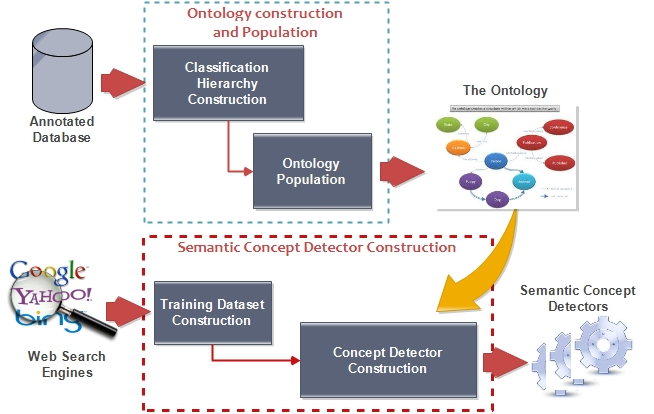
\includegraphics[scale=0.7]{graphics/contrib3:figure1}
		\caption{Ontology based semantic annotator hierarchy for image annotation}
		\label{fig1}
	\end{figure}

	Image annotation is considered as a multi-class classification problem. 
	Many approaches were proposed to handle the annotation scalability aspect 
	(large number of \revAnglais{concepts} to annotate with) through combining semantic hierarchical
	structures with classification techniques (like \textsc{Svm} : Support Vector Machine)
	\citep{Cevikalp2010,Li2010,Bannour2012,McNamara2015}.
	Mainly, two different approaches were proposed for constructing the semantic hierarchy. 
	The first one is qualified as top-down method: the semantic hierarchy is \revAnglais{built} through
	recursive class set clustering \citep{Cevikalp2010}. The second one is qualified as
	bottom-up method: the hierarchy is  defined by agglomerative partitioning of the classes
	\citep{Li2010}. Furthermore, two different approaches were proposed also for hierarchical
	image classification: the first is the \textit{Binary Hierarchical Decision Trees} 
	(\textsc{Bhdts})\citep{Cevikalp2010}, and the second is the \textit{Decision Directed 
	Acyclic Graphs} (\textsc{Ddags}) \citep{Gao2011}.

	Let $C = \{c_{1} , c_{2}  , \dots , c_{N}\}$ be a set of $N$ semantic concept. 
	The \textsc{Ddags} approach trains $N * (N-1)/2$ binary classifiers and uses a 
	\textsc{DAG} to decide if an image $image$ belongs or not to a semantic concept 
	class $c_{i} \in C$. At each given node at a distance $d$ from the tree root, $d$
	semantic concept classes are eliminated, and $N-d$ decision nodes remain to be evaluated. 
	The \textsc{Bhdts} approach \revAnglais{handles} the semantic hierarchy as a binary tree: concept 
	classes are clustered hierarchically into two subsets. This clustering step is iterated 
	until a single concept class set is reached. For every clustering step,  an \textsc{Svm} 
	classifier is trained in order to decide if an image $image$ could be annotated by the first or 
	the opposite semantic concept class. A total of $log_{2}(N)$ \textsc{Svm} classifiers are 
	trained and used for analyzing a test image.  Despite the fact that these two approaches enable 
	accurate classifiers, they handle semantic hierarchy as binary structures which requests 
	a considerable structure to handle with large amount of concept classes.

	Considering that \textsc{Bhdt} approach aims to optimize the \textsc{SVM} classifiers 
	accuracy through reducing the unnecessary comparisons \citep{Cevikalp2010}, 
	we are motivated to use such an \revAnglais{approach} in our scalable image annotation framework.

	In our proposed framework, we aim to define a new method for constructing a hierarchical 
	classifiers for scalable image annotation. At first, an annotated image dataset is analyzed to 
	construct the hierarchy tree for concept classes. Then, and for every level of the defined 
	tree structure, an \textsc{Svm} is trained for predicting if a test image $image$ belongs 
	to the first concept class set or the second one. By starting by the first level  (root node), 
	the hierarchy is walked until reaching leafs nodes through computing classifier votes  (see figure \ref{fig3_2}).

	\begin{figure}[ht!]
		\centering
		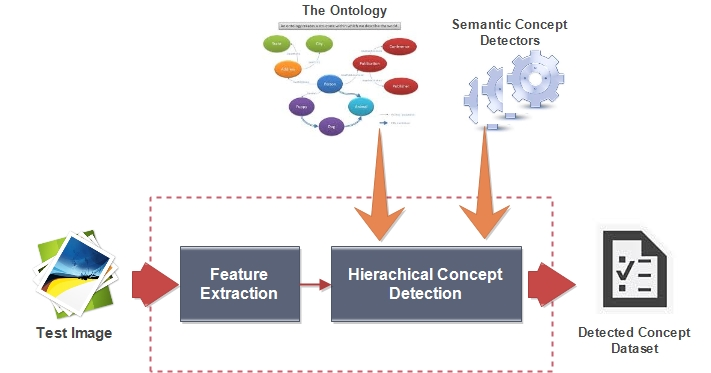
\includegraphics[scale=0.7]{graphics/contrib3:figure2}
		\caption{Ontology based Hierarchical image classification}
		\label{fig3_2}
	\end{figure}

	Our method is inspired from fuzzy decision tree based method \citep{Wang2015,Bujnowski2015} 
	to extract uncertain knowledge in a classification problem. Fuzzy set theory is used to model
	the tree structure. Thus, our proposed approach is based on a fuzzy ontology that handles such 
	a decision tree. In what follows, we discuss the structure of our fuzzy ontology, we show how 
	we populate its content, and how to infer available knowledge in order to use the hierarchical 
	classifiers to annotate a test image accurately.

	\subsection{Ontology Structure}
		The ontology structure is based on three conceptual \revAnglais{classes:} the semantic 
		concept $\mathsf{Concept}$, the hierarchical node $\mathsf{Node}$, and the test image $\mathsf{Image}$.
		We define also a set of relationships between these conceptual classes (see table \ref{tab1}).
		\begin{table}[ht!]
			\centering
			\caption{Semantic Relationships between conceptual classes}
			\begin{tabular}{ c c p{5cm}  }
			\hline
			\textbf{\small Relationships} 	& \textbf{\small Definition}	&\textbf{\small Meaning} \\
			\hline \hline
			
			$\mathsf{isIndexedBy}$	& 
			$(\langle{}\mathsf{Image},\mathsf{Concept}\rangle:\mathsf{isIndexedBy}) \geq p_{1}$ 
			& The image $\mathsf{Image}$ is annotated by the concept $\mathsf{Concept}$ by a fuzzy weight $p_{1}$  \\
			\hline
			
			$\mathsf{votesFor}$		& 
			$(\langle{}\mathsf{Node},\mathsf{Image}\rangle:\mathsf{votesFor}) \geq p_{2}$ 
			& The \textsc{Svm} for the node $\mathsf{Node}$ votes for the image $\mathsf{image}$ by a fuzzy weight $p_{2}$  \\
			\hline
	
			$\mathsf{existsIn}$		& 
			$(\langle{}\mathsf{Concept},\mathsf{Node}\rangle:\mathsf{existsIn}) \geq p_{3}$ 
			& The image $\mathsf{image}$ exists in the node $\mathsf{Node}$ by a fuzzy weight $p_{3}$  \\
			\hline
	
			$\mathsf{isChildOf}$	& 
			$(\langle{}\mathsf{Node},\mathsf{Node}\rangle:\mathsf{isChildOf})$ 
			& The first node $\mathsf{Node}$ has a semantic concept subset of the second node 
			$\mathsf{Node}$ \\
			\hline
		\end{tabular}
		\label{tab1}
	\end{table}


The relationship $\mathsf{isChildOf}$ depicts that a node $node_{1} \in \mathsf{Node}$ is a child of another node $node_{2} \in \mathsf{Node}$. This relationship is used then for modeling the semantic hierarchy for concept classes.

The relationship $\mathsf{existsIn}$ enumerates for each node $node \in \mathsf{Node}$ the contained set of concept classes. A concept $concept \in \mathsf{Concept}$ can \revAnglais{exist} in many nodes, but for separate levels.
 
The relationship $\mathsf{votesFor}$ is used when an image $image$ is being annotated and the hierarchy is walked from the root node to the leafs. A node $node \in \mathsf{Node}$ votes for an image $image \in \mathsf{Image}$ by a fuzzy weight $p_{2}$ when a \textsc{Svm} classification on that image predicts that the image $image$ could \revAnglais{be }annotated by the set of semantic concepts that exists in the node $node$.
	
Finally, the relationship $\mathsf{isIndexedBy}$ depicts that an image $image \in \mathsf{Image}$ is annotated by the concept $concept \in \mathsf{Concept}$ by a fuzzy weight equal to $p_{1}$.
		
The proposed ontology structure is used to enable handling the hierarchical classifiers, to trace the hierarchy walk for classifying a given test image, and then to model the set of semantic concepts that annotate that image (see figure \ref{fig3}). In what follows, we expose the population process for our ontology, then, we discuss the reasoning process used to guide and assist the hierarchical annotation.


\begin{figure}[ht!]
	\centering
	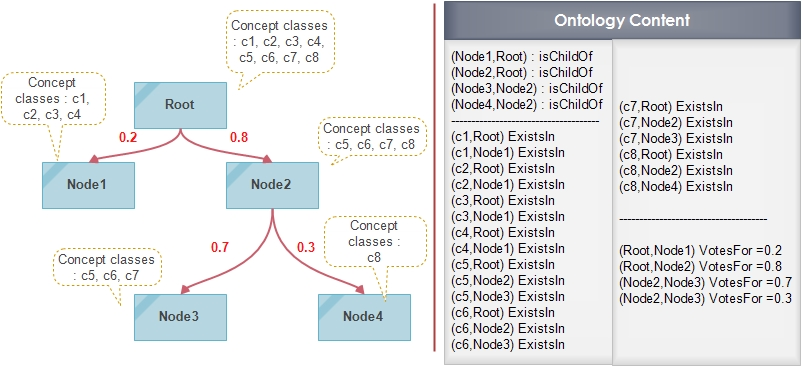
\includegraphics[scale=0.72]{graphics/contrib3:structure}
	\caption{Ontological Hierarchy content for image annotation}
	\label{fig3}
\end{figure}
		\subsection{Ontology population}
		
Given a defined set of semantic concepts, we start by clustering it through analyzing annotated image dataset provided by the \textit{ImageCLEF 2015 Scalable Concept Image Annotation} task.  

At first, we apply a binary clustering for the whole concept set, and we define two new nodes in the ontology $node_{1}$ and $node_{2}$.
We use a \textit{k-means} clustering algorithm with $k=2$.
 Then, each concept is instantiated within the ontology, and for every concept $concept$ that belongs to the node $node$, a new relationship $\mathsf{existsIn}$ is instantiated between $concept$ and $node$. This process is recursively called on $node_{1}$ and $node_{2}$ until a sub-node contains only one semantic concept class, or the clustering process seems unable to cluster a given semantic concept classes. At each iteration, the new defined nodes are populated within the ontology through instantiating the $\mathsf{isChildOf}$ relationships. 

		\subsection{Hierarchical classificators construction}

Once the hierarchical structure is defined through the above mentioned recursive binary clustering, an \textsc{Svm} based classifier is trained for all the nodes that belong to the same level. As training images, we select some development images for every concept that belongs to a node. In section \ref{label1}, we detail the development image dataset used for the training task.

\begin{figure}[ht!]
	\centering
	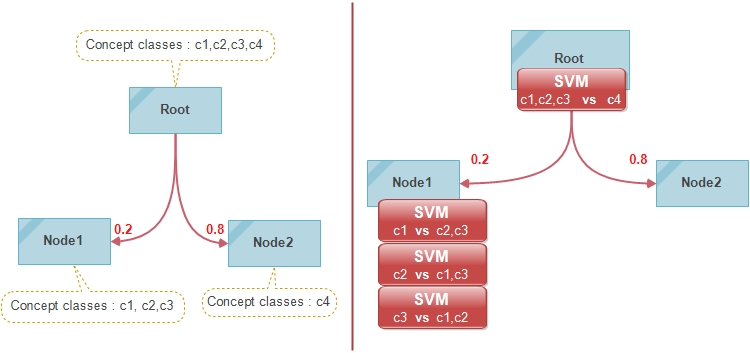
\includegraphics[scale=0.8]{graphics/contrib3:figure3}
	\caption{Hierarchical SVM classificator construction}
	\label{fig4}
\end{figure}

At a given level, two possible nodes are figuring (see figure \ref{fig4}). By exploring $\mathsf{existsIn}$ relationships, we construct a training image dataset. For the first node (see node \emph{Root} in figure \ref{fig4}), and for each concept that belongs to that node, a subset of images that are annotated by this concept are selected to be training images for corresponding node.

For a leaf node (see node \emph{Node1} in figure \ref{fig4}), we proceed as follow: let $C_{m} = \{ c_{1}, c_{2}, \dots, c_{k}\}$ be a set of $k$ concepts that belongs to the node $node_{m}$. We construct then $k$ classifiers. Each classifier is related to a given concept and trained against the other concepts. Then, and for a classifier $f$ of a concept $c_{f} \in C_{m}$, we train an \textsc{Svm} classifier based on two image sets: the first set is based on images that are annotated by the concept $c_{f}$, and the other set is based on images that are annotated by the other concepts ($C_{m} \setminus c_{f}$).

For a leaf node that \revAnglais{contains} only one concept class (see node \emph{Node2} in figure \ref{fig4}), no \textsc{Svm} classifier will be constructed. And an image annotation for this concept will be computed through the leaf node classification vote.

		\subsection{Reasoning}

We start reasoning from the root node (top node) of the constructed fuzzy tree (see figure \ref{fig3}). For a given node, we compute the values of the membership functions ($\mu$) for the child nodes through firing the corresponding \textsc{Svm} classifiers. The classification results (the vote) are populated into the fuzzy ontology through instantiating the $\mathsf{votesFor}$ relationship.

%Cheng2010
%Chen2009
In order to improve reasoning accuracy and to minimize the decision tree walk (which will also minimize the number of \textsc{Svm} classifiers to be fired), we define a \textit{Fuzziness control threshold} $\theta_{r} = 0.1$: given two sub-nodes $node_{1}$ 
and $node_{2}$, firing the \textsc{Svm} classifier at this level provides two membership function values $\mu_{1}$ for $node_{1}$ and  $\mu_{2}$ for $node_{2}$. Then, we compute $\theta_{r} = | \mu_{1} - \mu_{2} |$.

if $\theta_{r} \leq 0.1$, then we could not be sure if the \textsc{Svm} classifier is discriminative to judge if the content of a test image belongs to the first or to the second node. We proceed so to walk both sub-nodes ($node_{1}$ and $node_{2}$). For the opposite case ($\theta_{r} > 0.1$), the reasoner walks only the node that has the greater membership function value ($\mu$). 

Given the example in figure \ref{fig3}, the \textsc{Svm} classifier of the node $root$ computed $\mu_{1} = 0.2$ for the node $Node1$, and 
$\mu_{2} = 0.8$ for the node $Node2$. Then, the reasoning algorithm stops walking the node $Node1$ and proceeds to walk the $Node2$ since
$\theta_{r} = 0.8-0.2 = 0.6$ and $0.1 \leq 0.6$.

A leaf node can contain a set of concept classes, or only one concept class. In the first case, and for every contained concept class, an \textsc{Svm} classifier is fired for that concept against the other contained concept classes. The classification result is populated in the ontology through the instantiation of the relationship $\mathsf{isIndexedBy}$ between the concept class and the test image. The fuzzy weight for the new relationship is computed as an average of $\mu$ values computed from the root node to the leaf one. 
 In case of a single concept class, a new $\mathsf{isIndexedBy}$ relationship is instantiated within the ontology between that concept and the test image. The fuzzy weight \revAnglais{is computed} as in the first case.

Our proposed fuzzy decision tree reasoner assists the annotation of a given test image through firing recursive trained \textsc{Svm} classifiers in order to optimize the number of concept to be detected. Such an optimization should reduce also the computing cost of a given test image annotation process.

In the next section, we expose how we construct an \textsc{Svm} classifier for each node in the constructed fuzzy hierarchical semantic structure of concept classes.


	%%%%%%%%%%%%%%%%%%%%%%%%%%%%%%%%%%%%%%%%%%%%%%%%%%%%%%%%%%%%%%%%%%%%%%%%%%%%%%%%%%%%%%%%%%%%%%%%%%%%%
	\section{Experiments and Results}
	\label{c3_3}
		
		In this section, we discuss the obtained experimental results from our participation in the 
		\textit{Imageclef 2015} (within the \textit{Scalable Concept Image Annotation} task).
		In such an experiment, we look particularly in the assessment of our approach scalability, 
		rather than the semantic enhancement.
		
		In the rest of this section, we start by presenting the used dataset and metrics for 
		the evaluation, we, then, show how we build hierarchical concept detectors in accordance 
		with what was presented in the previous section. And finally, we discuss the obtained results.

		\subsection{Datasets Description}
			The image dataset provided by the \textit{ImageClef 2015} evaluation campaign is 
			constructed through querying popular search engines (mainly \textsc{Google}, \textsc{Bing} 
			and \textsc{Yahoo!}). A total of $500~000$ images \revAnglais{were} gathered \citep{Gilbert2015}.

			The test dataset contains all the defined $500~000$ images. And the development dataset 
			contains $5~520$ annotated images taken from the test dataset. A total of $251$ semantic
			concepts where used to annotated the content of the development set of images.

			For each image in the dataset, a full text description of the image content is 
			provided through extracting text content from the web-page where the image is located.

		\subsection{Evaluation metrics}
			In \textit{imageclef 2015} \textit{Scalable Concept Image Annotation} task, the annotation 
			accuracy is evaluated using the \textsc{Map} metric.
			
			Another metric is used: the \textsc{Pascal Voc} \citep{Everingham2015}. But the 
			latter evaluates not only the annotation accuracy, but also the semantic 
			concept localization. Since our approach \revAnglais{desn't} handle yet such \revAnglais{an} ability, 
			we consider only the \textsc{Map} metric.


		%%%%%%%%%%%%%%%%%%%%%%%%%%%%%%%%%%%%%%%%%%%%%%%%%%%%%%%%%%%%%%%%%%%%%%%%%%%%%%%%%%%%%%%%%%%%%%%%%%%%%
		\subsection{\textsc{Svm} Classifier Construction}
			In our participation within \textit{ImageCLEF 2015 Scalable Concept Image Annotation} task,
			we aimed basically to evaluate the scalability aspect of our preliminary automatic annotation 
			framework. For semantic concept detector/annotator, we have not really defined an original approach, 
			but we implemented state-of-the-art bags of quantized local features and linear 
			classifiers learned by support vector machines. In fact, and as pointed in \cite{Piras2014}, 
			bag-of-features and codebook approach has 
			gained a great attention by image classification and annotation community 
			as it showed notable semantic accuracy 
			\citep{Jurie2005,Gemert2008,Mylonas2009,Ngo2010,Grana2013,Hidaka2013,Kanehira2014,Xu2014,Elleuch2015}.
			%\cite{Mylonas2009,Kanehira2014,Elleuch2015}.
			In what follow, we expose how we construct \textsc{Svm} classifiers for semantic concept detection and annotation.

			\subsubsection{Construct a learning dataset}
				\label{label1}
				Image annotation has always been heavily dependent \revAnglais{on} good development datasets. 
				First, datasets were mainly hand-collected. However, and recently, several researches 
				attempt to automate such a laborious task. Re-ranking images gathered from popular 
				Image search engines (\textsc{Google}, \textsc{Yahoo!}, \textsc{Bing}, \dots) 
				can construct automatically an image learning dataset \citep{Fergus2004,Fergus2005,Schroff2011}.

				As a development dataset, we have not used one provided by the \textit{ImageCLEF
				2015 Scalable Concept Image Annotation task}. In fact, not all the concepts were annotated. 
				We relied then on \textsc{Flickr} image search engine to obtain image set and construct 
				a learning dataset. We used so the information provided with concept list to 
				query the search engine and we gathered first 100 result images for each given concept.

				At the outset, it seems to be curious to use an external data source as a development dataset. 
				Our aim is to explore available on-line data-sources (like search engines) to train non 
				annotated semantic concepts.


			\subsubsection{Local Feature Extraction}
				Our framework extracts \revAnglais{feature} from an input image through a robust local feature extractor.
				We followed a basic and state-of-the-art framework for such purpose (as described in \citep{Piras2014}).
				Leading extractors for such a purpose \revAnglais{include} \textit{Scale Invariant Feature 
				Transform} (\textsc{Sift}) and \textit{Speeded Up Robust Features} (\textsc{Surf}).
				Local feature descriptors handle a pixel within an image by analyzing 
				its neighborhood pixels. Many different descriptors and interest-point
				detectors were proposed and discussed in the literature. While the \textsc{Sift} 
				descriptor \citep{Lowe2004} is considered as the most widely used descriptor, 
				\textsc{Surf}  \citep{Bay2008} is known as robust local feature extraction
				to various image perturbations.

				Our framework extracts local features and descriptors using \textsc{Surf}. Such a choice is
				argued by \textsc{Surf} concise descriptor length (64 floating point values).
				The \textsc{Surf} implementation that we used is provided by 
				\textsc{OpenCv} \citep{Bradski2008}.

				For query image analysis, local features are extracted and mapped into 
				nearest computed cluster centroids. The query image is then handled by a 
				vector that represents defined visual bag-of-words.

			\subsubsection{Classification of local Features and Constructing the bag-of-words model}
				After extracting local features, a bag-of-words model is used to represent these descriptors. 
				The \revAnglais{latters} are extracted from training images and are grouped into $N$ clusters of 
				visual words using \textit{k-means}.	
				Each  defined descriptor is classified into its cluster centroid by computing the 
				\textit{Euclidean distance} metric. For our runs, we choose a value of $N = 100$. 
				This value is argued by a balance between high bias (under-fitting) and high variance (over-fitting).
				
				In order to alleviate the computing cost of \textit{k-means} clustering, we used 
				\textit{Mini Batch k-means} 
				\cite{Sculley2010} as an alternative to the \textit{k-means} algorithm for clustering massive 
				datasets. \textit{Mini Batch k-means} reduces the computational cost by handling fixed size 
				subsample instead of all the data in the database. This strategy reduces the amount 
				of distance to be computed at each clustering iteration.

			\subsubsection{Learning Algorithm}
				The learning algorithm consists in training one-vs.-one linear \textsc{Svm}
				to operate in the bag of \textsc{Surf} feature space. Training images are classified
				through a histogram vector conctructed in the \textit{k-means} based clustering.
				We used a linear kernel for our \textsc{Svm} based learning algorithm in view of its simplicity and 					computational efficiency in training and classification: $K(x,y) = x^{T}y+c$.

				Basically, \textsc{Svm} are binary classifier. For a given detector, an image 
				is annotated by one of two distinct groups. A one-vs.-one scheme is used in which 
				each \textsc{Svm} trained for each combination of individual classes. 
				The \textsc{Svm} implementation used in our runs is given by \textsc{Scikit-Learn} 
				library \citep{Pedregosa2011}.

			\subsubsection{Decision}

				As an \textsc{Svm} decision function, a class membership probability estimation 
				fits the decision values.
		
				\textsc{Scikit-Learn} library uses a \textsc{Platt Scaling} in order to 
				calibrate the \textsc{Svm} classifier to produce, in addition to class 
				predictions, probabilities. When the \textsc{Svm} is trained, an optimization 
				process is called to optimize parameter vectors $A$ and $B$ such \revAnglais{that:}
				$P(y|X) = 1/ (1+exp(A*f(X) + B))$ where $f(X)$ 
				is the signed distance of a sample  from the hyperplane.

			

		\subsection{Experiments with \textit{ImageClef 2015}}

			Our goal behind our participation in \textit{ImageClef 2012} is to assess the proposed 
			ontology based hierarchical concept detection scalability. However, and unlike the 
			scalability assessment presented in the previous chapter (where we tested the 
			scalability of the system to handle a large-scale image dataset), we aim to test if 
			our approach could be scalable when the number of semantic concepts \revAnglais{increases}. Our idea 
			behind the ontology based hierarchical concept detection consists in filtering the 
			concepts to be detected: not all the concept detectors will be called in the detection process.



			\subsubsection{Image Semantic Annotation Evaluation}
			For the image annotation, we only annotated only $300~000$ images of 
			the $500~000$ images provided in the test dataset. Furthermore, we used just 
			low resolution images (thunbnail)
			instead of the full resolution images. In fact, the large amount \revAnglais{of} images to 
			be annotated has forced us to reduce the quality of processed images in the 
			aim to accelerate the annotation computational cost. Yet, we haven't \revAnglais{proceeded
			to annotate} the full image dataset (only $300.000$ images).

			The tables \ref{tabres1} and \ref{tabres2} display the obtained results in terms of
			semantic annotation accuracy. We think that a full size image dataset annotation with
			more tweaked \textsc{Svm} classifiers should give better results. 
			Furthermore, fuzzy ontology based semantic enhancement (described in the previous 
			chapter \citep{Zarka2015}) should also enhance our framework annotation accuracy.

			\begin{table}[ht]
				\centering
				\caption{\textsc{ImageClef 2015}: $MAP\_0\_Overlap$ Runs evaluation}
				\begin{tabular}{ l| l l }
				\hline
				\textbf{\small } 	& \textbf{\small MAP} &	 \\
				\hline \hline
		
				\textbf{\small Best run}  & {\small $0,795403$}	& {\small(/SMIVA/21.run)} \\
				\textbf{\small Worst run} & {\small$0,0305398$}	& 
					{} \\
				\textbf{\small Average}	  & {\small$0,31046$} 	&  \\
				\textbf{\small Our best run~~}& {\small$0,0366072$} 	&  {\small(position $85/89$)} \\
				\hline
				\end{tabular}
				
				\label{tabres1}
			\end{table}

			\begin{table}[ht]
				\centering
				\caption{\textsc{ImageClef 2015}: $MAP\_0.5\_Overlap$ Runs evaluation}
				\begin{tabular}{ l| l l }
				\hline
				\textbf{\small } 	& \textbf{\small MAP} &	 \\
				\hline \hline
				\textbf{\small Best run}  & {\small $0,659507$}		& {\small(/SMIVA/21.run)} \\
				\textbf{\small Worst run} & {\small $0,000231898$}	& {\small(} \\
				\textbf{\small Average}	  & {\small $0,18673$} 		&  \\
				\textbf{\small Our best run~~}& {\small$0,0161687$} 	&  {\small(position $75/89$)} \\
				\hline
				\end{tabular}
				
				\label{tabres2}
			\end{table}

			As illustrated in tables \ref{tabres1} and \ref{tabres2}, the system \textsc{Smiva} 
			\citep{Pravin2015} showed great annotation performance. This system annotates images
			not only in the basis of its visual content, but also through analyzing textual information 
			in the web page where the analyzed image is localized. For our evaluation, we only used visual analysis.


			
			\subsubsection{Scalability Evaluation}

			We would remind that our objective is to alleviate the computation cost of the 
			image annotation through a proposed framework that is based on an ontology 
			reasoning driven hierarchical concept detector.

			For the training process, we trained the \textsc{Svm} classifiers in about $100$ hours
			(we used 100 learning images per a concept). This task was executed on 
			a \revAnglais{modern} machine (Intel $i5$ processor with $16$ GB RAM memory).
	
			The annotation task was done on $10$ machines (each one has one core 
			CPU and $1$ GB of RAM). The annotation of $300~000$ images elapsed about $1~633$ hours 
			(without taking into consideration the \textsc{Vps} parallel computing).

			Our framework annotates a test image with an average of $19.615$ seconds (the maximum record 
			was $597.250$ seconds and the minimum one was $0.066$ second). 
			And for a given test image, an average of $52$ \textsc{Svm} classifiers were fired
			(the maximum was $175$ and the minimum was $6$). Our framework has reduced 
			the number of \textsc{Svm} classifiers to be fired in order to annotate a given test image.

			We can conclude that our proposed framework reduced the number of requested semantic 
			concept detector to annotate an image: from $251$ concept detectors, to an average of $52$
			ones. Then, the time required to annotate an image is decreased by $80\%$





	%%%%%%%%%%%%%%%%%%%%%%%%%%%%%%%%%%%%%%%%%%%%%%%%%%%%%%%%%%%%%%%%%%%%%%%%%%%%%%%%%%%%%%%%%%%%%%%%%%%%%
	\section{Conclusion}
	\label{c3_4}

	In this chapter note, we described our annotation framework for scalable ontology driven 
	semantic image annotation. We discussed our ontology based framework for reducing the number of 
	concepts to be detected for a given image. We developed a state-of-the art bag-of-words based 
	concept detector (that uses \textsc{Surf} feature extractor and \textit{k-means} classification).
	Then, concept detectors are selected through reasoning with a fuzzy ontology content. Thus, not all 
	the concept detectors are used for a given image. 

% 	In our experiment, we showed how the use of such a method could reduce the number of concept 
% 	detectors to be used in order to efficiently annotate a large-scale image dataset. While the 
% 	obtained results were not really impressive, we still believe 
% 	that our framework can reveal better results through tweaking local feature extraction and
% 	training, and exploiting semantic enhancement through fuzzy reasoning. 
% 	Thus, we are considering potential future directions to further improve our proposed framework. 
	
	The main discussed contribution was to propose a scalable framework for
		multimedia content analysis. We focused then on the use of an ontology in order to construct 
		fast semantic concept detectors. Although the promising obtained results, we believe that the
		implementation of these constructed detectors within \emph{Hadoop/MapReduce} and even \emph{GPU} 
		based runtime-environment (like \textsc{Cuda, OpenCL} \citep{Mahmoudi2015,Osipyan2015,Dantas2015,Peters2015}
		could enable more efficiency for multimedia content analysis.



			
	\part{Conclusions and Future Research Directions}
			\chapter{Conclusions and Perspectives}
\label{conlusion}

	The general framework of this dissertation is video information retrieval. 
	The main tackled challenge is how to enable a user to easily access and interpret 
	video contents. Particularly, our thesis works are focused on a contextual 
	concept-based video indexing that represents a motivating solution to such a challenge. 
	The major inherent difficulty in this task is the semantic gap: what separates the signal
	representation from semantics (concept, contexts and relationships).

	In multimedia indexing and retrieval literature, the multimedia community primarily focused
	on concept model building through a supervised learning technique that analyzes the extracted 
	low-level features: representative features vectors are extracted from a set of representative 
	manually annotated data (commonly images), then used  for a supervised learning algorithm in order 
	to approach the semantic interpretation. Nevertheless, such an approach partially solved the semantic gap 
	problem: it is difficult to detect efficiently a variety of concepts, and still unable to detect 
	implicit objects (semantic concepts that do not figure in the content, or that \revAnglais{cannot} be easily 
	detected). On the one hand, such issues are induced by the large variety of semantics that could be handled, 
	on the other hand, the inability of these approaches taking into consideration semantic concept relationships.
	Thus, recent research works are focusing on using ontologies for multimedia retrieval in order
	to allow semantic interpretation and reasoning over extracted descriptions. However, much
	remains to be done in order to achieve less human aid ontology modeling approaches.

	\section{Summary of Contributions}

	Our thesis work proposed a generic and scalable fuzzy knowledge based framework to enhance 
	concept-based multimedia indexing. In this context, our contributions aim to improve the accuracy, 
	the scalability and the generalization capability of our semantic video indexing system: \textsc{RegimVid}. 
	These novelties are enumerated as follows: 
	(1) a new knowledge based model for multimedia indexing. 
	The objective is to develop a framework able to handle various information about a multimedia content, 
	then to operate with \revAnglais{this} information in order to infer new information/knowledge through a reasoning process. 
	Such a novel model has to define and highlight pertinent components for an efficient knowledge based indexing process.
	(2) an ontology based framework to handle fuzzy knowledge and reason with semantic interpretations 
	in order to enhance and enrich them. This objective aims to define a semantic structure to model 
	required knowledge, then to specify an automated ontology population from available annotated 
	image/video datasets, and finally to handle ontology content evolving to further improve 
	semantics capabilities through \revAnglais{analyzing} and revising inaccurate and irrelevant knowledge.
	(3) an approach for an automatic multimedia indexing by the use of an ontology-based semantic 
	hierarchy handled at both learning and annotation steps. 

	While recent works focused on the use of semantic hierarchies to improve concept detector accuracy, 
	this objective means the use of such hierarchies to reduce detector complexity and then, to handle 
	efficiently large-scale multimedia datasets.


%%%%%%%%%%%%%%%%%%%%%%%%%%%%%%%
	\section{Future Research Directions}
	Many approaches were proposed in this dissertation in order to deal with video indexing 
	issues. Indeed, the semantic gap problem remains an open problem and could not be solved in 
	the near future. Therefore, research works on video indexing are witnessing an incremental
	improvement, and many supplementary efforts are still needed.

	In the following, we discuss some potential future directions that could be explored further over 
	the described achievements throughout this dissertation.

\begin{description}
	\item[Fuzzy Similarities]   Defining ontologies content was based on computing similarities 
		between concepts granted by a large annotated images dataset. Although we used the 
		statistical \emph{cosine} similarity function, more advanced fuzzy similarity 
		functions \citep{Baccour2013,Baccour2014} could be addressed in order to handle real 
		fuzzy knowledge to be inserted in proposed ontologies.
% 	\item[]    The ontology evolving approach proposed for our fuzzy ontology-based 
% 		system is quite preliminary. However, ontology evolving evaluation showed promising 
% 		results and proved that such an ontology revision should lead to a more pertinent 
% 		knowledge, then a better semantic interpretation enhancement. 
% 		Thus, we consider that extensive research works on 
% 		the ontology evolving part of our proposed approach should be more tackled.
	\item[Video genre]   We proposed a \revAnglais{knowledge} structure that enhances the accuracy of a semantic \revAnglais{interpretation}.
		Nevertheless, when analyzing a video annotated dataset, all videos are handled as if they were addressing the same subject. 
		Furthermore, the videos can be classified according to their genres. Thus, the relationships between 
		concepts/contexts can differ from one genre to another, and \revAnglais{subsequently}, from one video to another.
		In literature, the video classification is well-addressed 
		(\citep{Wu2012, Huang2012, Chattopadhyay2013, Muneesawang2014} to cite a few). 
		We are convinced that addressing the video genre as a semantic information can 
		further refine the extracted fuzzy relationships, and consequently, the video semantic 
		interpretation enhancement. Thus, we consider that it could be an interesting task that 
		should be followed for a future work. 
	\item[Big data video analysis ] 
		\revKarray{Many research works considers deep neural networks as a powerful
		 framework for big data video repositories
		 \citep{Girshick2014,Jiang2015,Sainath2015,Tong2015}. 
		 In \citep{Wu2015,Druzhkov2016}, a comprehensive survey on deep learning
		 and neural networks based approaches for video analysis and indexing is discussed.
		 The effectiveness  of such approaches resides in exploring parallel processing 
		 units (such as \textsc{Cuda} based machines \citep{Osipyan2015}) to run the 
		 neural networks pipelines. However, and as discussed in section 3.4, we are 
		 focusing more in our thesis work on a knowledge-based approach rather than 
		 a parallel one. }
		 
		 \revKarray{As a third contribution (discussed in chapter 6), we showed that a knowledge-based 
		 approach could reduce the computing cost of semantic concept detectors. 
		 But, we believe that this contribution should 
		 be extended to deep neural networks in order to achieve robust and real time 
		 multimedia content analysis.   }	
	
	\item[Domain Adaptation and Ontology evolving] 
		\revKarray{Ontology evolving is an important step in an ontology construction. 
		In fact, this step ensures not only the accuracy of the managed knowledge, but leads also to a continuous 
		adaptation of an ontology to a variety of application domains. The latter is based on the use of particular 
		approaches for constructing a discriminative model within a shift between observed data (training) and 
		analyzed one (test). Such a situation is widely discussed particularly when dealing with big data where 
		information is diverse and heterogeneous, and defined as \textit{domain adaptation} \citep{Pan2010}. 
		Many approaches were discussed in literature for the domain adaptation mainly by bridging the learned 
		(observed) and target (analyzed) domains by learning domain invariant features : the classifier learned 
		from observed domain can then be applied to the target domain \citep{Long2016}.}

		\revKarray{Recent studies are focusing particularly on deep neural networks to handle invariant features for domain 
		adaptation \citep{Donahue2014,Yosinski2014,Kumar2016}. Indeed, the domain adaptation is embedded in the pipeline 
		of deep feature learning in order to extract domain invariant representation 
		\citep{Tzeng2014,Long2015}.}

		\revKarray{In multimedia analysis, the domain adaptation leads to alleviate manual construction of 
		labeled data, and to enhance the ability to handle extended domains 
		\citep{Saenko2010,Gopalan2011,Gong2012,Duan2012a,Hoffman2014,Liu2016}. 
		Some recent works addressed the domain adaptation with more focus on deep neural networks 
		\citep{Ganin2015,Tzeng2015}.}

		\revKarray{Thus, the domain adaptation is an interesting research direction that should be tackled when 
		dealing with ontology population and evolving. In the present dissertation, we  opted to 
		use classical approaches to extract and evolve the content of an ontology. Thereby, 
		we believe that such a research direction will be highly considered as a future work.}

\end{description}

%	 \section{Future Development Directions}
%
%	\revKarray{As discussed in the previous section, the research presented in this dissertation 
%	leaves many promising avenues open for future research. This section looks at some 
%	of the future directions in the development of the multimedia retrieval systems.}
%
%	\revKarray{As hand-held and mobile devices are becoming common, the proposed framework to enhance
%	a semantic interpretation and to alleviate the complexity of semantic concept detection could 
%	be integrated within these devices. In fact, the use of semantic hierarchies to improve concept
%	detector accuracy could not only to handle efficiently large-scale multimedia contents, 
%	but also to enable efficient visual indexing with limited power and memory devices. 
%	Then, the semantic enhancement could enrich and improve incomplete semantic interpretation
%	using the ontology's deduction capabilities.}
%
%	\revKarray{For such a purpose, the proposed framework needs to be optimized so that it can be processed
%	with less power and memory capabilities.}

	



\appendix

%\chapter{Annex A}

%\chapter{Annex B}



%-------------------------------------------------------------------
%              L'index
%-------------------------------------------------------------------

% à ajouter

%-------------------------------------------------------------------
%                       La bibliographie
%-------------------------------------------------------------------

% La bibliographie 
\setstretch{1.3}
\bibliographyfancy
\bibliography{bibliography/mybib2}

%%%\newpage ~
\newpage \pagestyle{empty} ~

%\chapter*{Author's Response \\ to the Reviewers' Comments}

% ======================================================= %
%\noindent Dear editor and reviewers,\\

	We would like to thank the reviewers for their interest in our work and their
	relevant and helpful comments that will greatly improve and velarize the thesis manuscript. 
	Thus, we tried to do our best to respond to the raised points. 

	The reviewers have brought up good comments and the opportunity 
	to clarify our research objectives and results. In this document, we have
	checked all the comments provided by the reviewers and have made necessary 
	changes according polo 2017to their recommendations.

	For clarity, the comments are applied in the new thesis manuscript version 
	with \colorbox{babyblue}{\textsf{Blue}} color for the reviewer Professor Fakhri Karray, 
	with \colorbox{brightgreen}{\textsf{Green}} color for the reviewer Professor Sami Faiz, 
	and finally with \colorbox{yellow}{\textsf{Yellow}} color for typos and editorial mistakes.

	\vfill
	Yours sincerely, Mohamed ZARKA.


	\newpage

% ======================================================= %
\section*{Answers to reviewer: Professor Fakhri Karray}

\question{There	are several typos and editorial	mistakes and strongly recommend the candidate to carefully proofread the thesis.} 

\answer We apologize for the typos and the editorial misyakes. They were considered and corrected.


\question{The candidate made very good literature review and has highlighted recent work in the field. 
	Possibly more would have been proposed especially recent approaches highlighted in the literature dealing
	with big data based video clip repositories indexing and search using on-line learning and domain adaptation. 
	This is a very promising research direction and would wish to have the candidate mention 
	it as future potential direction.}

\answer ...


\question{The examiner would have wished to see more powerful performance metric such as recall performance 
	and computation requirement (algorithmic time performance).}

\answer ...

\question{Moreover, it is very important when dealing 
	with large data set to apply distributed/cloud computing environment to handle real-time classification
	and detection of new concepts/relationship. This requires a certain type of the algorithm structure, 
	not mentioned in details in this work. These are major issue on their own, and it is not expected 
	the candidate to deal with all of them here. He	simply needs to highlight them though in the final draft.}

\answer ...

\question{Hybrid approaches using existing solid techniques for concept detection coupled with machine learning
	algorithms to deal with concept relationship (context) is being proven very powerful. 
	Candidate should mention these approaches in his references.}

\answer ...


\question{I have some issues with the publication record (in terms of quantity and quality) 
	and strongly suggest that the candidate should really work hard on publishing his work in 
	well-known venues pertinent to the field.}

\answer We thank you for pointing this out. 

	In terms of publication quality, we published our second contribution within a well known journal 
	(Springer MTAP with impact factor of $1.331$). Actually, I am drafting a second journal paper that 
	deals with our third contribution in order to valorize the obtained results. 
	Yet, I target the following two journals for the submission:
	\textit{ACM Multimedia Computing, Communications, and Applications} (Impact Factor of $2.465$),
	or \textit{Springer International Journal of Computer Vision} (Impact Factor of $4.270$).

	In terms of publication quantity, I would like to notice that handling large amount of data was a 
	real hard task with the use of very classical computing machines. I will try to do my best to 
	increase my publication rate. Thank you again for this comment.

	As for industrial development, we prepared a patent  INNORPI (National Institute of 
	Standardization and Industrial Property). This patent is entitled \textit{“Dispositif d'Enrichissement 
	Sémantique en utilisant des ONTOlogies (DESONTO) pour l'amélioration de l'indexation des 
	contenus multimédias”}, and it details the semantic enhancement for multimedia retrieval systems 
	through the use of fuzzy ontologies (as described in our second contribution C2). 
	This patent is currently under review. 
	Furthermore, we are preparing a second patent about the scalability aspect. 
	This patent is entitled \textit{“Annotation Sémantique Rapide des Images en utilisant des Ontologies 
	(ASRIO) pour l'indexation des contenus visuels.”}, 
	and it proposes an alleviated computing task for semantic concept detection within multimedia contents. 
	This patent is being drafted.

	In order to highlight such a promising industrial development, we added a new section entitled 
	“\textit{7.3 Future Development Directions}” in the chapter “\textit{Conclusions and Perspectives}”.

% ==================================================================================================== %
% ==================================================================================================== %        
% ==================================================================================================== %        
% ==================================================================================================== %        
% ==================================================================================================== %        
% ==================================================================================================== %        
% ==================================================================================================== % 

\setcounter{commentNum}{0}
\section*{Answers to Reviewer: Professor Sami Faiz}

\question{Nous aurions juste aimé avoir une discussion au cas où les connaissances pouvant être elles mêmes floues.}




%\newpage ~
\newpage \pagestyle{empty} ~

\incgraph[documentpaper,
  overlay={\node[red] at (page.center) {};}]
  [width=\paperwidth,height=\paperheight]{resumes/RESUMES.jpg}

%\newpage \pagestyle{empty} ~
%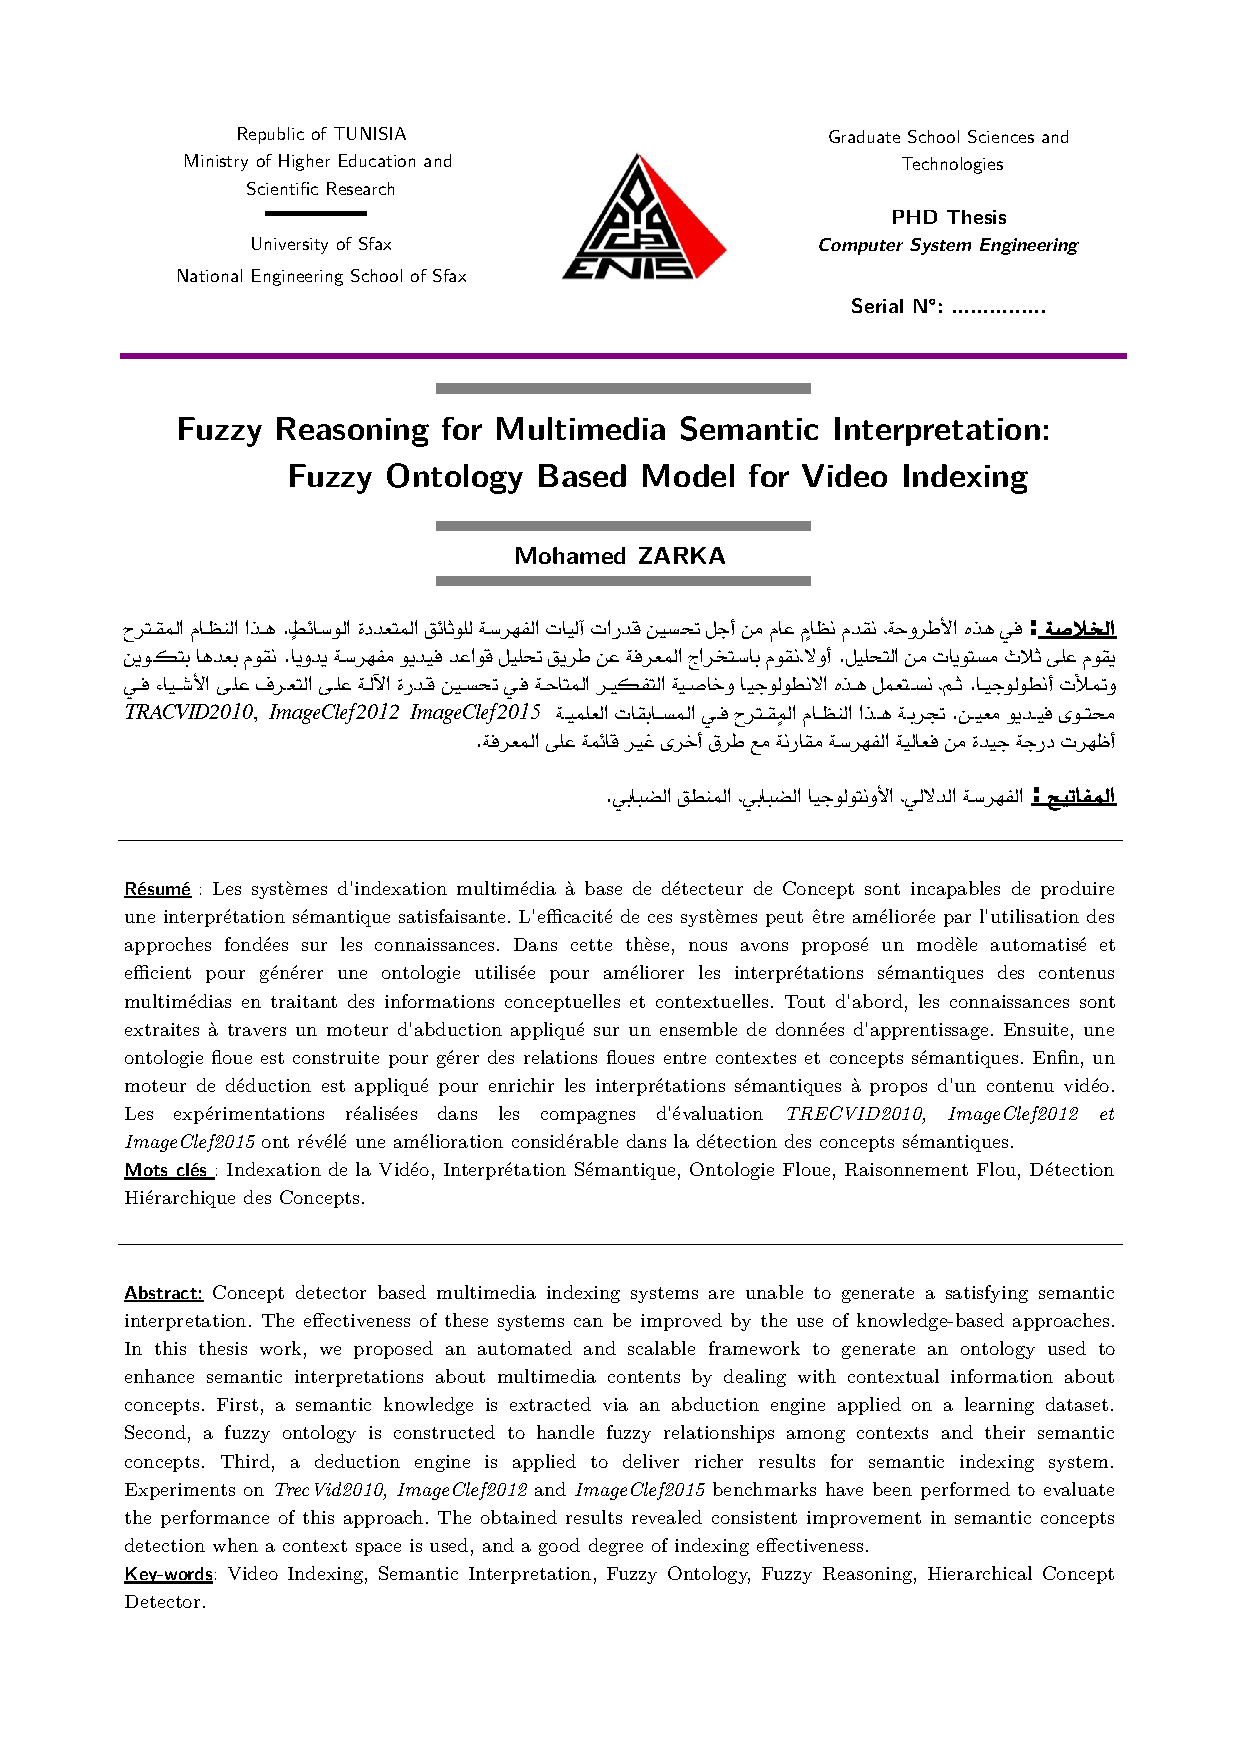
\includepdf[pages=1]{resumes/RESUMES.pdf}

\end{document}
